% This is the Reed College LaTeX thesis template. Most of the work 
% for the document class was done by Sam Noble (SN), as well as this
% template. Later comments etc. by Ben Salzberg (BTS). Additional
% restructuring and APA support by Jess Youngberg (JY).
% Your comments and suggestions are more than welcome; please email
% them to cus@reed.edu
%
% See http://web.reed.edu/cis/help/latex.html for help. There are a 
% great bunch of help pages there, with notes on
% getting started, bibtex, etc. Go there and read it if you're not
% already familiar with LaTeX.
%
% Any line that starts with a percent symbol is a comment. 
% They won't show up in the document, and are useful for notes 
% to yourself and explaining commands. 
% Commenting also removes a line from the document; 
% very handy for troubleshooting problems. -BTS

% As far as I know, this follows the requirements laid out in 
% the 2002-2003 Senior Handbook. Ask a librarian to check the 
% document before binding. -SN

%%
%% Preamble
%%
% \documentclass{<something>} must begin each LaTeX document
\documentclass[12pt,twoside]{reedthesis}
% Packages are extensions to the basic LaTeX functions. Whatever you
% want to typeset, there is probably a package out there for it.
% Chemistry (chemtex), screenplays, you name it.
% Check out CTAN to see: http://www.ctan.org/
%%
\usepackage{graphicx, latexsym} 
\usepackage{amssymb,amsthm,amsmath,algorithm}
\usepackage{longtable,booktabs,setspace} 
\usepackage[hyphens]{url}
\usepackage{rotating}
\usepackage{natbib}
\usepackage{cleveref}
\usepackage{paralist}
\usepackage{algpseudocode}
\usepackage{pstricks}
% \usepackage[T1]{fontenc}
% \usepackage{epstopdf}
\usepackage{dirtytalk}
\usepackage{subcaption}
\usepackage{wrapfig}
\captionsetup{format=hang,justification=raggedright}
% \usepackage{minipage}
\graphicspath{ {figs/} }
\makeatletter
\let\OldStatex\Statex
\renewcommand{\Statex}[1][3]{%
  \setlength\@tempdima{\algorithmicindent}%
  \OldStatex\hskip\dimexpr#1\@tempdima\relax}
\makeatother
% Comment out the natbib line above and uncomment the following two lines to use the new 
% biblatex-chicago style, for Chicago A. Also make some changes at the end where the 
% bibliography is included. 
%\usepackage{biblatex-chicago}
%\bibliography{thesis}

% \usepackage{times} % other fonts are available like times, bookman, charter, palatino

\title{the big paper, if you will}
\author{Isabella F. Jorissen}
% The month and year that you submit your FINAL draft TO THE LIBRARY (May or December)
\date{May 2016}
\division{Mathematics and Natural Sciences}
\advisor{James Fix}
%If you have two advisors for some reason, you can use the following
%\altadvisor{Your Other Advisor}
%%% Remember to use the correct department!
\department{Mathematics}
% if you're writing a thesis in an interdisciplinary major,
% uncomment the line below and change the text as appropriate.
% check the Senior Handbook if unsure.
%\thedivisionof{The Established Interdisciplinary Committee for}
% if you want the approval page to say "Approved for the Committee",
% uncomment the next line
%\approvedforthe{Committee}
% \newtheorem{def}{Definition}
\setlength{\parskip}{0pt}
%%
%% End Preamble
%%
%% The fun begins:
\begin{document}

  \maketitle
  \frontmatter % this stuff will be roman-numbered
  \pagestyle{empty} % this removes page numbers from the frontmatter

% Acknowledgements (Acceptable American spelling) are optional
% So are Acknowledgments (proper English spelling)
    \chapter*{Acknowledgements}
	I want to thank a few (lots, really) people.

% The preface is optional
% To remove it, comment it out or delete it.
    \chapter*{Preface}
    [I'm going to tell you a story about a math problem. There will be some words (don't worry about their meaning too much), some concepts (the words will help some), and a few pretty diagrams (to pull it all together). This is a story about a lot of things, depending on your perspective. In a way, it's a story about figuring out where you ought to go based on where you are. At least, that one of the ways I like to think about it. I've thrown in a little High Performance Computing for good measure, since - if you're anything like me - you'll want to know where your destination is as quickly as possible.

    This math problem has a lot of names, and has been discovered, re-discovered, named, re-named, used, and re-used in more disciplines than I'm willing to count or list. I'd argue that the ``conceptual'' ``mathematical'' structure itself ``belongs'' to the realm of Computational Geometry, where it's referred to as the Voronoi Diagram. It has many aliases: Dirichlet Tesselation, Thiessen Polygons, Plant Polygons, and Wigner-Seitz Cell, among others. 

    In the names of Tradition and Clarity, I've done my best to use exoteric language whenever possible, and to indulge in mathematical notation where appropriate. You're welcome to treat either as an endless stream of notation. My only advice to you, in the words of a Reed math professor I once had: ``remain calm.'']

    % \begin {figure}
    %   \begin{center}
    %   % Define new PST objects, if not already defined
\ifx\PSTloaded\undefined
\def\PSTloaded{t}
\psset{arrowsize=.01 3.2 1.4 .3}
\psset{dotsize=.1}
\catcode`@=11

\newpsobject{PST@Border}{psline}{linewidth=.0015,linestyle=solid}
\newpsobject{PST@Axes}{psline}{linewidth=.0015,linestyle=dotted,dotsep=.004}
\newpsobject{PST@Solid}{psline}{linewidth=.0015,linestyle=solid}
\newpsobject{PST@Dashed}{psline}{linewidth=.0015,linestyle=dashed,dash=.01 .01}
\newpsobject{PST@Dotted}{psline}{linewidth=.0025,linestyle=dotted,dotsep=.008}
\newpsobject{PST@LongDash}{psline}{linewidth=.0015,linestyle=dashed,dash=.02 .01}
\newpsobject{PST@Diamond}{psdots}{linewidth=.001,linestyle=solid,dotstyle=square,dotangle=45}
\newpsobject{PST@Filldiamond}{psdots}{linewidth=.001,linestyle=solid,dotstyle=square*,dotangle=45}
\newpsobject{PST@Cross}{psdots}{linewidth=.001,linestyle=solid,dotstyle=+,dotangle=45}
\newpsobject{PST@Plus}{psdots}{linewidth=.001,linestyle=solid,dotstyle=+}
\newpsobject{PST@Square}{psdots}{linewidth=.001,linestyle=solid,dotstyle=square}
\newpsobject{PST@Circle}{psdots}{linewidth=.05,linestyle=solid,dotstyle=o}
\newpsobject{PST@Triangle}{psdots}{linewidth=.001,linestyle=solid,dotstyle=triangle}
\newpsobject{PST@Pentagon}{psdots}{linewidth=.001,linestyle=solid,dotstyle=pentagon}
\newpsobject{PST@Fillsquare}{psdots}{linewidth=.001,linestyle=solid,dotstyle=square*}
\newpsobject{PST@Fillcircle}{psdots}{linewidth=.002,linestyle=solid,dotstyle=*}
\newpsobject{PST@Filltriangle}{psdots}{linewidth=.001,linestyle=solid,dotstyle=triangle*}
\newpsobject{PST@Fillpentagon}{psdots}{linewidth=.001,linestyle=solid,dotstyle=pentagon*}
\newpsobject{PST@Arrow}{psline}{linewidth=.001,linestyle=solid}
\catcode`@=12

\fi
\psset{unit=5.0in,xunit=5.0in,yunit=3.0in}
\pspicture(0.000000,0.000000)(1.000000,1.000000)
\ifx\nofigs\undefined
\catcode`@=11

\PST@Border(0.0400,0.9679)
(0.0400,0.0320)
(0.9519,0.0320)
(0.9519,0.9679)
(0.0400,0.9679)

% \rput[r](0.8099,0.9229){'results/edges.dat'}
% \PST@Border(0.8259,0.9229)
% (0.9199,0.9229)

\PST@Border(0.3895,0.5843)
(0.3895,0.5843)
(0.4698,0.5890)

\PST@Border(0.4601,0.4729)
(0.4601,0.4729)
(0.6049,0.0320)

\PST@Border(0.4884,0.5082)
(0.4884,0.5082)
(0.9519,0.4746)

\PST@Border(0.4884,0.5082)
(0.4884,0.5082)
(0.4698,0.5890)

\PST@Border(0.4698,0.5890)
(0.4698,0.5890)
(0.3895,0.5843)

\PST@Border(0.4884,0.5082)
(0.4884,0.5082)
(0.9519,0.4746)

\PST@Border(0.4698,0.5890)
(0.4698,0.5890)
(0.6339,0.8119)

\PST@Border(0.3971,0.4777)
(0.3971,0.4777)
(0.1891,0.0320)

\PST@Border(0.3971,0.4777)
(0.3971,0.4777)
(0.4601,0.4729)

\PST@Border(0.3971,0.4777)
(0.3971,0.4777)
(0.3675,0.5172)

\PST@Border(0.4601,0.4729)
(0.4601,0.4729)
(0.3971,0.4777)

\PST@Border(0.3675,0.5172)
(0.3675,0.5172)
(0.3895,0.5843)

\PST@Border(0.4601,0.4729)
(0.4601,0.4729)
(0.4884,0.5082)

\PST@Border(0.4884,0.5082)
(0.4884,0.5082)
(0.4601,0.4729)

\PST@Border(0.3895,0.5843)
(0.3895,0.5843)
(0.3675,0.5172)

\PST@Border(0.4698,0.5890)
(0.4698,0.5890)
(0.4884,0.5082)

\PST@Border(0.4698,0.5890)
(0.4698,0.5890)
(0.6339,0.8119)

\PST@Border(0.3675,0.5172)
(0.3675,0.5172)
(0.0400,0.4870)

\PST@Border(0.3971,0.4777)
(0.3971,0.4777)
(0.1891,0.0320)

\PST@Border(0.3895,0.5843)
(0.3895,0.5843)
(0.2280,0.8119)

\PST@Border(0.3675,0.5172)
(0.3675,0.5172)
(0.3971,0.4777)

\PST@Border(0.3895,0.5843)
(0.3895,0.5843)
(0.2280,0.8119)

\PST@Border(0.3675,0.5172)
(0.3675,0.5172)
(0.0400,0.4870)

\PST@Border(0.4601,0.4729)
(0.4601,0.4729)
(0.6049,0.0320)

% \rput[r](0.8099,0.8729){'results/sites.dat' using 1:2}
\PST@Fillcircle(0.4295,0.5329)
\PST@Fillcircle(0.3273,0.5682)
\PST@Fillcircle(0.4235,0.6401)
\PST@Fillcircle(0.5304,0.5572)
\PST@Fillcircle(0.5233,0.4536)
\PST@Fillcircle(0.4211,0.4183)
\PST@Fillcircle(0.3368,0.4597)
\PST@Fillcircle(0.8729,0.8729)
% \rput[r](0.8099,0.8229){'results/vertices.dat' using 1:2}
\PST@Circle(0.4698,0.5890)
\PST@Circle(0.3895,0.5843)
\PST@Circle(0.3675,0.5172)
\PST@Circle(0.4884,0.5082)
\PST@Circle(0.3971,0.4777)
\PST@Circle(0.4601,0.4729)
\PST@Circle(0.8729,0.8229)
\PST@Border(0.0400,0.9679)
(0.0400,0.0320)
(0.9519,0.0320)
(0.9519,0.9679)
(0.0400,0.9679)

\catcode`@=12
\fi
\endpspicture
    %   \end{center}
    % \end {figure}


    % \begin {figure}
    %   \begin{center}
    %   \caption{check this ish out... now put it in illustrator to make it pretty n such}
    %   % GNUPLOT: LaTeX picture using PSTRICKS macros
% Define new PST objects, if not already defined
\ifx\PSTloaded\undefined
\def\PSTloaded{t}
\psset{arrowsize=.01 3.2 1.4 .3}
\psset{dotsize=.2}
\catcode`@=11

\newpsobject{PST@Border}{psline}{linewidth=.0015,linestyle=solid}
\newpsobject{PST@Axes}{psline}{linewidth=.0015,linestyle=dotted,dotsep=.004}
\newpsobject{PST@Solid}{psline}{linewidth=.0015,linestyle=solid}
\newpsobject{PST@Dashed}{psline}{linewidth=.0015,linestyle=dashed,dash=.01 .01}
\newpsobject{PST@Dotted}{psline}{linewidth=.0025,linestyle=dotted,dotsep=.008}
\newpsobject{PST@LongDash}{psline}{linewidth=.0015,linestyle=dashed,dash=.02 .01}
\newpsobject{PST@Diamond}{psdots}{linewidth=.001,linestyle=solid,dotstyle=square,dotangle=45}
\newpsobject{PST@Filldiamond}{psdots}{linewidth=.001,linestyle=solid,dotstyle=square*,dotangle=45}
\newpsobject{PST@Cross}{psdots}{linewidth=.001,linestyle=solid,dotstyle=+,dotangle=45}
\newpsobject{PST@Plus}{psdots}{linewidth=.001,linestyle=solid,dotstyle=+}
\newpsobject{PST@Square}{psdots}{linewidth=.001,linestyle=solid,dotstyle=square}
\newpsobject{PST@Circle}{psdots}{linewidth=.001,linestyle=solid,dotstyle=o}
\newpsobject{PST@Triangle}{psdots}{linewidth=.001,linestyle=solid,dotstyle=triangle}
\newpsobject{PST@Pentagon}{psdots}{linewidth=.001,linestyle=solid,dotstyle=pentagon}
\newpsobject{PST@Fillsquare}{psdots}{linewidth=.001,linestyle=solid,dotstyle=square*}
\newpsobject{PST@Fillcircle}{psdots}{linewidth=.001,linestyle=solid,dotstyle=*}
\newpsobject{PST@Filltriangle}{psdots}{linewidth=.001,linestyle=solid,dotstyle=triangle*}
\newpsobject{PST@Fillpentagon}{psdots}{linewidth=.001,linestyle=solid,dotstyle=pentagon*}
\newpsobject{PST@Arrow}{psline}{linewidth=.001,linestyle=solid}
\catcode`@=12

\fi
\psset{unit=5.0in,xunit=5.0in,yunit=3.0in}
\pspicture(0.000000,0.000000)(1.000000,1.000000)
\ifx\nofigs\undefined
\catcode`@=11

\PST@Border(0.0400,0.9679)
(0.0400,0.0320)
(0.9519,0.0320)
(0.9519,0.9679)
(0.0400,0.9679)

\PST@Border(0.5919,0.8296)
(0.5919,0.8296)
(0.5678,0.7622)

\PST@Border(0.5632,0.8780)
(0.5632,0.8780)
(0.5979,0.9679)

\PST@Border(0.4347,0.7782)
(0.4347,0.7782)
(0.1686,0.9679)

\PST@Border(0.6599,0.6032)
(0.6599,0.6032)
(0.5678,0.7622)

\PST@Border(0.5919,0.8296)
(0.5919,0.8296)
(0.5632,0.8780)

\PST@Border(0.4963,0.8871)
(0.4963,0.8871)
(0.5632,0.8780)

\PST@Border(0.4347,0.7782)
(0.4347,0.7782)
(0.4490,0.7462)

\PST@Border(0.7487,0.8441)
(0.7487,0.8441)
(0.5919,0.8296)

\PST@Border(0.4963,0.8871)
(0.4963,0.8871)
(0.4249,0.9679)

\PST@Border(0.4490,0.7462)
(0.4490,0.7462)
(0.5678,0.7622)

\PST@Border(0.4963,0.8871)
(0.4963,0.8871)
(0.4347,0.7782)

\PST@Border(0.7487,0.8441)
(0.7487,0.8441)
(0.9088,0.9679)

\PST@Border(0.5632,0.8780)
(0.5632,0.8780)
(0.5979,0.9679)

\PST@Border(0.5678,0.7622)
(0.5678,0.7622)
(0.6599,0.6032)

\PST@Border(0.5632,0.8780)
(0.5632,0.8780)
(0.4963,0.8871)

\PST@Border(0.6599,0.6032)
(0.6599,0.6032)
(0.7238,0.0320)

\PST@Border(0.6599,0.6032)
(0.6599,0.6032)
(0.7487,0.8441)

\PST@Border(0.7487,0.8441)
(0.7487,0.8441)
(0.6599,0.6032)

\PST@Border(0.5632,0.8780)
(0.5632,0.8780)
(0.5919,0.8296)

\PST@Border(0.5919,0.8296)
(0.5919,0.8296)
(0.7487,0.8441)

\PST@Border(0.7487,0.8441)
(0.7487,0.8441)
(0.9088,0.9679)

\PST@Border(0.5678,0.7622)
(0.5678,0.7622)
(0.4490,0.7462)

\PST@Border(0.4963,0.8871)
(0.4963,0.8871)
(0.4249,0.9679)

\PST@Border(0.4347,0.7782)
(0.4347,0.7782)
(0.4963,0.8871)

\PST@Border(0.4347,0.7782)
(0.4347,0.7782)
(0.1686,0.9679)

\PST@Border(0.4490,0.7462)
(0.4490,0.7462)
(0.2138,0.0320)

\PST@Border(0.4490,0.7462)
(0.4490,0.7462)
(0.2138,0.0320)

\PST@Border(0.6599,0.6032)
(0.6599,0.6032)
(0.7238,0.0320)

\PST@Border(0.4490,0.7462)
(0.4490,0.7462)
(0.4347,0.7782)

\PST@Border(0.5678,0.7622)
(0.5678,0.7622)
(0.5919,0.8296)

\PST@Fillcircle(0.3558,0.7485)
\PST@Fillcircle(0.5244,0.9484)
\PST@Fillcircle(0.7726,0.7193)
\PST@Fillcircle(0.5244,0.6901)
\PST@Fillcircle(0.4342,0.8643)
\PST@Fillcircle(0.5078,0.8204)
\PST@Fillcircle(0.6384,0.9021)
\PST@Fillcircle(0.6503,0.7668)

\PST@Circle(0.4963,0.8871)
\PST@Circle(0.5632,0.8780)
\PST@Circle(0.5919,0.8296)
\PST@Circle(0.7487,0.8441)
\PST@Circle(0.4347,0.7782)
\PST@Circle(0.5678,0.7622)
\PST@Circle(0.4490,0.7462)
\PST@Circle(0.6599,0.6032)
\PST@Border(0.0400,0.9679)
(0.0400,0.0320)
(0.9519,0.0320)
(0.9519,0.9679)
(0.0400,0.9679)

\catcode`@=12
\fi
\endpspicture
    %   \end{center}
    % \end {figure}

    % \begin {figure}
    %   \begin{center}
    %   \caption{check this ish out... now put it in illustrator to make it pretty n such}
    %   
% Define new PST objects, if not already defined
\ifx\PSTloaded\undefined
\def\PSTloaded{t}

\fi
\psset{unit=1in,xunit=1in,yunit=1in}
\pspicture(-1.000000,-1.000000)(1.000000,1.000000)
\ifx\nofigs\undefined
\catcode`@=11

\def\RightHalfEdgeCCW{
  \psline[liftpen=2, linearc=.008]{-}(0.05, 0.0)(1.2, 0.0)(.90,.15)
}

\def\LeftHalfEdgeCCW{
  \psline[liftpen=2, linearc=.005]{-}(0.95, 0.0)(0.0, 0.0)(.20,.12)
}



% labels
\rput[t](.6,.15){$e$}
\rput[t](.6,-.15){$e.twin$}
\rput[t]{120}(.75,.4){$e.next$}
% central one
\pscustom[linewidth=1.5pt]{
\msave
  \RightHalfEdgeCCW
  \translate(1.225,.025)
  \rotate{120}
  \RightHalfEdgeCCW
  \translate(1.225,.025)
  \rotate{120}
  \RightHalfEdgeCCW
} 

% bottom
\pscustom[linewidth=1.5pt, linecolor=darkgray]{
  \mrestore
  \msave
  \rotate{180}
  \translate(-1.2, .1)
  \RightHalfEdgeCCW
  \translate(1.225,.025)
  \rotate{120}
  \RightHalfEdgeCCW
  \translate(1.225,.025)
  \rotate{120}
  \RightHalfEdgeCCW
}


% left
\pscustom[linewidth=1.5pt, linecolor=darkgray]{
  \mrestore
  \msave
  \translate(-0.05, 0.0)
  \rotate{180}
  \translate(-.5, -1.1)
  \RightHalfEdgeCCW
  \translate(1.225,.025)
  \rotate{120}
  \RightHalfEdgeCCW
  \translate(1.225,.025)
  \rotate{120}
  \RightHalfEdgeCCW
  % \mrestore
} 
% right
\pscustom[linewidth=1.5pt, linecolor=darkgray]{
  \mrestore
  \translate(0.05, 0.0)
  \rotate{180}
  \translate(-1.9, -1.1)
  \RightHalfEdgeCCW
  \translate(1.225,.025)
  \rotate{120}
  \RightHalfEdgeCCW
  \translate(1.225,.025)
  \rotate{120}
  \RightHalfEdgeCCW
}


\catcode`@=12
\fi
\endpspicture

    %   \end{center}
    % \end {figure}


    % \begin {figure}
    %   \begin{center}
    %   \caption{test results}
    %   % GNUPLOT: LaTeX picture using PSTRICKS macros
% Define new PST objects, if not already defined
\ifx\PSTloaded\undefined
\def\PSTloaded{t}
\psset{arrowsize=.01 3.2 1.4 .3}
\psset{dotsize=.2}
\catcode`@=11

\newpsobject{PST@Border}{psline}{linewidth=.0015,linestyle=solid}
\newpsobject{PST@Axes}{psline}{linewidth=.0015,linestyle=dotted,dotsep=.004}
\newpsobject{PST@Solid}{psline}{linewidth=.0015,linestyle=solid}
\newpsobject{PST@Dashed}{psline}{linewidth=.0015,linestyle=dashed,dash=.01 .01}
\newpsobject{PST@Dotted}{psline}{linewidth=.0025,linestyle=dotted,dotsep=.008}
\newpsobject{PST@LongDash}{psline}{linewidth=.0015,linestyle=dashed,dash=.02 .01}
\newpsobject{PST@Diamond}{psdots}{linewidth=.001,linestyle=solid,dotstyle=square,dotangle=45}
\newpsobject{PST@Filldiamond}{psdots}{linewidth=.001,linestyle=solid,dotstyle=square*,dotangle=45}
\newpsobject{PST@Cross}{psdots}{linewidth=.001,linestyle=solid,dotstyle=+,dotangle=45}
\newpsobject{PST@Plus}{psdots}{linewidth=.001,linestyle=solid,dotstyle=+}
\newpsobject{PST@Square}{psdots}{linewidth=.001,linestyle=solid,dotstyle=square}
\newpsobject{PST@Circle}{psdots}{linewidth=.001,linestyle=solid,dotstyle=o}
\newpsobject{PST@Triangle}{psdots}{linewidth=.001,linestyle=solid,dotstyle=triangle}
\newpsobject{PST@Pentagon}{psdots}{linewidth=.001,linestyle=solid,dotstyle=pentagon}
\newpsobject{PST@Fillsquare}{psdots}{linewidth=.001,linestyle=solid,dotstyle=square*}
\newpsobject{PST@Fillcircle}{psdots}{linewidth=.001,linestyle=solid,dotstyle=*}
\newpsobject{PST@Filltriangle}{psdots}{linewidth=.001,linestyle=solid,dotstyle=triangle*}
\newpsobject{PST@Fillpentagon}{psdots}{linewidth=.001,linestyle=solid,dotstyle=pentagon*}
\newpsobject{PST@Arrow}{psline}{linewidth=.001,linestyle=solid}
\catcode`@=12

\fi
\psset{unit=4.0in,xunit=5.0in,yunit=3.0in}
\pspicture(0.000000,0.000000)(1.000000,1.000000)
\ifx\nofigs\undefined
\catcode`@=11

\PST@Border(0.0000,0.0000)
(0.9999,0.0000)
(0.9999,0.9999)
(0.0000,0.9999)
(0.0000,0.0000)

\rput[l](0.0320,0.9580){pstricks  terminal test}
\rput[l](0.0320,0.9055){gnuplot version 5.0.1  }
\PST@Axes(0.5000,0.0000)
(0.5000,0.9999)

\PST@Axes(0.0000,0.5000)
(0.9999,0.5000)

\PST@Border(0.3400,0.5210)
(0.6600,0.5210)
(0.6600,0.4790)
(0.3400,0.4790)
(0.3400,0.5210)

\rput[l](0.3400,0.5000){12345678901234567890}
\rput[l](0.3400,0.5588){test of character width:}
\rput[l](0.5000,0.7520){left justified}
\rput(0.5000,0.7100){centre+d text}
\rput[r](0.5000,0.6680){right justified}
\rput{L}(0.0420,0.5000){rotated ce+ntred text}
\rput[l]{L}(0.1260,0.5000){ rotated by +45 deg}
\rput[l]{L}(0.0840,0.5000){ rotated by -45 deg}
\PST@Dotted(0.5300,0.9999)
(0.5300,0.9800)

\PST@Dotted(0.5000,0.9600)
(0.5150,0.9600)

\rput[r](0.4840,0.9580){show ticscale}
\rput[r](0.8730,0.9580){-1}
\PST@Border(0.8890,0.9580)
(0.9530,0.9580)

\rput[r](0.8730,0.9160){0}
\PST@Axes(0.8890,0.9160)
(0.9530,0.9160)

\qdisk(0.9765,0.9160){0.0003}
\rput[r](0.8730,0.8740){1}
\PST@Border(0.8890,0.8740)
(0.9530,0.8740)

\PST@Diamond(0.9765,0.8740)
\rput[r](0.8730,0.8320){2}
\PST@Border(0.8890,0.8320)
(0.9530,0.8320)

\PST@Plus(0.9765,0.8320)
\rput[r](0.8730,0.7900){3}
\PST@Border(0.8890,0.7900)
(0.9530,0.7900)

\PST@Square(0.9765,0.7900)
\rput[r](0.8730,0.7480){4}
\PST@Border(0.8890,0.7480)
(0.9530,0.7480)

\PST@Cross(0.9765,0.7480)
\rput[r](0.8730,0.7060){5}
\PST@Border(0.8890,0.7060)
(0.9530,0.7060)

\PST@Circle(0.9765,0.7060)
\rput[r](0.8730,0.6640){6}
\PST@Border(0.8890,0.6640)
(0.9530,0.6640)

\PST@Triangle(0.9765,0.6640)
\rput[r](0.8730,0.6220){7}
\PST@Border(0.8890,0.6220)
(0.9530,0.6220)

\PST@Pentagon(0.9765,0.6220)
\rput[r](0.8730,0.5800){8}
\PST@Border(0.8890,0.5800)
(0.9530,0.5800)

\PST@Filldiamond(0.9765,0.5800)
\rput[r](0.8730,0.5380){9}
\PST@Border(0.8890,0.5380)
(0.9530,0.5380)

\PST@Fillsquare(0.9765,0.5380)
\rput[r](0.8730,0.4960){10}
\PST@Border(0.8890,0.4960)
(0.9530,0.4960)

\PST@Filltriangle(0.9765,0.4960)
\rput[r](0.8730,0.4540){11}
\PST@Border(0.8890,0.4540)
(0.9530,0.4540)

\PST@Fillcircle(0.9765,0.4540)
\rput[r](0.8730,0.4120){12}
\PST@Border(0.8890,0.4120)
(0.9530,0.4120)

\PST@Fillpentagon(0.9765,0.4120)
\rput[r](0.8730,0.3700){13}
\PST@Border(0.8890,0.3700)
(0.9530,0.3700)

\PST@Diamond(0.9765,0.3700)
\rput[r](0.8730,0.3280){14}
\PST@Border(0.8890,0.3280)
(0.9530,0.3280)

\PST@Plus(0.9765,0.3280)
\rput[r](0.8730,0.2860){15}
\PST@Border(0.8890,0.2860)
(0.9530,0.2860)

\PST@Square(0.9765,0.2860)
\rput[r](0.8730,0.2440){16}
\PST@Border(0.8890,0.2440)
(0.9530,0.2440)

\PST@Cross(0.9765,0.2440)
\rput[r](0.8730,0.2020){17}
\PST@Border(0.8890,0.2020)
(0.9530,0.2020)

\PST@Circle(0.9765,0.2020)
\rput[r](0.8730,0.1600){18}
\PST@Border(0.8890,0.1600)
(0.9530,0.1600)

\PST@Triangle(0.9765,0.1600)
\rput[r](0.8730,0.1180){19}
\PST@Border(0.8890,0.1180)
(0.9530,0.1180)

\PST@Pentagon(0.9765,0.1180)
\rput[r](0.8730,0.0760){20}
\PST@Border(0.8890,0.0760)
(0.9530,0.0760)

\PST@Filldiamond(0.9765,0.0760)
\PST@Arrow{->}(0.2800,0.5000)(0.3850,0.5000)
\PST@Arrow{->}(0.2800,0.5000)(0.1750,0.5000)
\PST@Arrow{->}(0.2800,0.5000)(0.2800,0.6400)
\PST@Arrow{->}(0.2800,0.5000)(0.2800,0.3600)
\PST@Arrow{->}(0.2050,0.4000)(0.3550,0.6000)
\PST@Arrow(0.2050,0.6000)(0.2800,0.5000)
\PST@Arrow{->}(0.2800,0.5000)(0.3550,0.4000)
\PST@Border(0.0750,0.0400)
(0.1750,0.0400)

\rput[l](0.1750,0.0400){  lw 1}
\PST@Border(0.0750,0.0800)
(0.1750,0.0800)

\rput[l](0.1750,0.0800){  lw 2}
\PST@Border(0.0750,0.1200)
(0.1750,0.1200)

\rput[l](0.1750,0.1200){  lw 3}
\PST@Border(0.0750,0.1600)
(0.1750,0.1600)

\rput[l](0.1750,0.1600){  lw 4}
\PST@Border(0.0750,0.2000)
(0.1750,0.2000)

\rput[l](0.1750,0.2000){  lw 5}
\PST@Border(0.0750,0.2400)
(0.1750,0.2400)

\rput[l](0.1750,0.2400){  lw 6}
\rput[l](0.0750,0.2800){linewidth}
\PST@Border(0.3000,0.0400)
(0.4000,0.0400)

\rput[l](0.4000,0.0400){  dt 0}
\PST@Dashed(0.3000,0.0800)
(0.4000,0.0800)

\rput[l](0.4000,0.0800){  dt 1}
\PST@Dotted(0.3000,0.1200)
(0.4000,0.1200)

\rput[l](0.4000,0.1200){  dt 2}
\PST@LongDash(0.3000,0.1600)
(0.4000,0.1600)

\rput[l](0.4000,0.1600){  dt 3}
\PST@Solid(0.3000,0.2000)
(0.4000,0.2000)

\rput[l](0.4000,0.2000){  dt 4}
\rput[l](0.3000,0.2400){dashtype}
\rput(0.6750,0.1880){pattern fill}
\PST@Border(0.5000,0.0000)
(0.5000,0.1250)
(0.5250,0.1250)
(0.5250,0.0000)
(0.5000,0.0000)

\rput(0.5125,0.1460){ 0}
\PST@Border(0.5375,0.0000)
(0.5375,0.1250)
(0.5625,0.1250)
(0.5625,0.0000)
(0.5375,0.0000)

\rput(0.5500,0.1460){ 1}
\PST@Border(0.5750,0.0000)
(0.5750,0.1250)
(0.6000,0.1250)
(0.6000,0.0000)
(0.5750,0.0000)

\rput(0.5875,0.1460){ 2}
\PST@Border(0.6125,0.0000)
(0.6125,0.1250)
(0.6375,0.1250)
(0.6375,0.0000)
(0.6125,0.0000)

\rput(0.6250,0.1460){ 3}
\PST@Border(0.6500,0.0000)
(0.6500,0.1250)
(0.6750,0.1250)
(0.6750,0.0000)
(0.6500,0.0000)

\rput(0.6625,0.1460){ 4}
\PST@Border(0.6875,0.0000)
(0.6875,0.1250)
(0.7125,0.1250)
(0.7125,0.0000)
(0.6875,0.0000)

\rput(0.7000,0.1460){ 5}
\PST@Border(0.7250,0.0000)
(0.7250,0.1250)
(0.7500,0.1250)
(0.7500,0.0000)
(0.7250,0.0000)

\rput(0.7375,0.1460){ 6}
\PST@Border(0.7625,0.0000)
(0.7625,0.1250)
(0.7875,0.1250)
(0.7875,0.0000)
(0.7625,0.0000)

\rput(0.7750,0.1460){ 7}
\PST@Border(0.8000,0.0000)
(0.8000,0.1250)
(0.8250,0.1250)
(0.8250,0.0000)
(0.8000,0.0000)

% \rput(0.8125,0.1460){ 8}
% \polypmIIId{0}(0.75,0.83)(0.725,0.8733)(0.675,0.8733)(0.65,0.83)(0.675,0.7866)(0.725,0.7866)(0.75,0.83)
% \polypmIIId{0}(0.8,0.805)(0.775,0.8483)(0.725,0.8483)(0.7,0.805)(0.725,0.7616)(0.775,0.7616)(0.8,0.805)
% \rput(0.7000,0.9010){filled polygons:}
\catcode`@=12
\fi
\endpspicture

    %   \end{center}
    % \end {figure}


    % \begin {figure}
    %   \begin{center}
    %   \caption{check this ish out... now put it in illustrator to make it pretty n such}
    %   % GNUPLOT: LaTeX picture using PSTRICKS macros
% Define new PST objects, if not already defined
\ifx\PSTloaded\undefined
\def\PSTloaded{t}
\psset{arrowsize=.01 3.2 1.4 .3}
\psset{dotsize=.2}
\catcode`@=11

\newpsobject{PST@Border}{psline}{linewidth=.0015,linestyle=solid}
\newpsobject{PST@Axes}{psline}{linewidth=.0015,linestyle=dotted,dotsep=.004}
\newpsobject{PST@Solid}{psline}{linewidth=.0015,linestyle=solid}
\newpsobject{PST@Dashed}{psline}{linewidth=.0015,linestyle=dashed,dash=.01 .01}
\newpsobject{PST@Dotted}{psline}{linewidth=.0025,linestyle=dotted,dotsep=.008}
\newpsobject{PST@LongDash}{psline}{linewidth=.0015,linestyle=dashed,dash=.02 .01}
\newpsobject{PST@Diamond}{psdots}{linewidth=.001,linestyle=solid,dotstyle=square,dotangle=45}
\newpsobject{PST@Filldiamond}{psdots}{linewidth=.001,linestyle=solid,dotstyle=square*,dotangle=45}
\newpsobject{PST@Cross}{psdots}{linewidth=.001,linestyle=solid,dotstyle=+,dotangle=45}
\newpsobject{PST@Plus}{psdots}{linewidth=.001,linestyle=solid,dotstyle=+}
\newpsobject{PST@Square}{psdots}{linewidth=.001,linestyle=solid,dotstyle=square}
\newpsobject{PST@Circle}{psdots}{linewidth=.001,linestyle=solid,dotstyle=o}
\newpsobject{PST@Triangle}{psdots}{linewidth=.001,linestyle=solid,dotstyle=triangle}
\newpsobject{PST@Pentagon}{psdots}{linewidth=.001,linestyle=solid,dotstyle=pentagon}
\newpsobject{PST@Fillsquare}{psdots}{linewidth=.001,linestyle=solid,dotstyle=square*}
\newpsobject{PST@Fillcircle}{psdots}{linewidth=.001,linestyle=solid,dotstyle=*}
\newpsobject{PST@Filltriangle}{psdots}{linewidth=.001,linestyle=solid,dotstyle=triangle*}
\newpsobject{PST@Fillpentagon}{psdots}{linewidth=.001,linestyle=solid,dotstyle=pentagon*}
\newpsobject{PST@Arrow}{psline}{linewidth=.001,linestyle=solid}
\catcode`@=12

\fi
\psset{unit=5.0in,xunit=5.0in,yunit=3.0in}
\pspicture(0.000000,0.000000)(1.000000,1.000000)
\ifx\nofigs\undefined
\catcode`@=11

\PST@Border(0.0400,0.9679)
(0.0400,0.0320)
(0.9519,0.0320)
(0.9519,0.9679)
(0.0400,0.9679)

\rput[r](0.8249,0.9269){'results/edges.dat'}
\PST@Border(0.8409,0.9269)
(0.9199,0.9269)

\PST@Border(0.4784,0.4022)
(0.4784,0.4022)
(0.3842,0.7263)

\PST@Border(0.7700,0.4680)
(0.7700,0.4680)
(0.4784,0.4022)

\PST@Border(0.8293,0.9575)
(0.8293,0.9575)
(0.9519,0.8660)

\PST@Border(0.2761,0.2470)
(0.2761,0.2470)
(0.2009,0.0320)

\PST@Border(0.4551,0.9131)
(0.4551,0.9131)
(0.6906,0.7590)

\PST@Border(0.1541,0.4041)
(0.1541,0.4041)
(0.2761,0.2470)

\PST@Border(0.2761,0.2470)
(0.2761,0.2470)
(0.4117,0.2649)

\PST@Border(0.6906,0.7590)
(0.6906,0.7590)
(0.7700,0.4680)

\PST@Border(0.1863,0.6282)
(0.1863,0.6282)
(0.0400,0.8086)

\PST@Border(0.1863,0.6282)
(0.1863,0.6282)
(0.3842,0.7263)

\PST@Border(0.1541,0.4041)
(0.1541,0.4041)
(0.0400,0.3642)

\PST@Border(0.4117,0.2649)
(0.4117,0.2649)
(0.4784,0.4022)

\PST@Border(0.1863,0.6282)
(0.1863,0.6282)
(0.0400,0.8086)

\PST@Border(0.3842,0.7263)
(0.3842,0.7263)
(0.4784,0.4022)

\PST@Border(0.7700,0.4680)
(0.7700,0.4680)
(0.9519,0.3046)

\PST@Border(0.4551,0.9131)
(0.4551,0.9131)
(0.4459,0.9679)

\PST@Border(0.4551,0.9131)
(0.4551,0.9131)
(0.4459,0.9679)

\PST@Border(0.6906,0.7590)
(0.6906,0.7590)
(0.8293,0.9575)

\PST@Border(0.3842,0.7263)
(0.3842,0.7263)
(0.1863,0.6282)

\PST@Border(0.6906,0.7590)
(0.6906,0.7590)
(0.4551,0.9131)

\PST@Border(0.8293,0.9575)
(0.8293,0.9575)
(0.8288,0.9679)

\PST@Border(0.4551,0.9131)
(0.4551,0.9131)
(0.3842,0.7263)

\PST@Border(0.4117,0.2649)
(0.4117,0.2649)
(0.5196,0.0320)

\PST@Border(0.4117,0.2649)
(0.4117,0.2649)
(0.5196,0.0320)

\PST@Border(0.8293,0.9575)
(0.8293,0.9575)
(0.6906,0.7590)

\PST@Border(0.1863,0.6282)
(0.1863,0.6282)
(0.1541,0.4041)

\PST@Border(0.1541,0.4041)
(0.1541,0.4041)
(0.1863,0.6282)

\PST@Border(0.8293,0.9575)
(0.8293,0.9575)
(0.9519,0.8660)

\PST@Border(0.7700,0.4680)
(0.7700,0.4680)
(0.9519,0.3046)

\PST@Border(0.1541,0.4041)
(0.1541,0.4041)
(0.0400,0.3642)

\PST@Border(0.8293,0.9575)
(0.8293,0.9575)
(0.8288,0.9679)

\PST@Border(0.4784,0.4022)
(0.4784,0.4022)
(0.4117,0.2649)

\PST@Border(0.2761,0.2470)
(0.2761,0.2470)
(0.1541,0.4041)

\PST@Border(0.4117,0.2649)
(0.4117,0.2649)
(0.2761,0.2470)

\PST@Border(0.4784,0.4022)
(0.4784,0.4022)
(0.7700,0.4680)

\PST@Border(0.2761,0.2470)
(0.2761,0.2470)
(0.2009,0.0320)

\PST@Border(0.7700,0.4680)
(0.7700,0.4680)
(0.6906,0.7590)

\PST@Border(0.3842,0.7263)
(0.3842,0.7263)
(0.4551,0.9131)

\rput[r](0.8249,0.8849){'results/sites.dat' using 1:2}
\PST@Plus(0.2185,0.8486)
\PST@Plus(0.5541,0.6150)
\PST@Plus(0.1004,0.1809)
\PST@Plus(0.6009,0.2342)
\PST@Plus(0.3160,0.4881)
\PST@Plus(0.8634,0.7699)
\PST@Plus(0.8804,0.8849)
\rput[r](0.8249,0.8429){'results/vertices.dat' using 1:2}
\PST@Square(0.8293,0.9575)
\PST@Square(0.4551,0.9131)
\PST@Square(0.6906,0.7590)
\PST@Square(0.3842,0.7263)
\PST@Square(0.1863,0.6282)
\PST@Square(0.1541,0.4041)
\PST@Square(0.4784,0.4022)
\PST@Square(0.7700,0.4680)
\PST@Square(0.4117,0.2649)
\PST@Square(0.2761,0.2470)
\PST@Square(0.8804,0.8429)
\PST@Border(0.0400,0.9679)
(0.0400,0.0320)
(0.9519,0.0320)
(0.9519,0.9679)
(0.0400,0.9679)

\catcode`@=12
\fi
\endpspicture
    %   \end{center}
    % \end {figure}


	% This is an example of a thesis setup to use the reed thesis document class.

    \tableofcontents
    \listofalgorithms
    \listoffigures

% The abstract is not required if you're writing a creative thesis (but aren't they all?)
% If your abstract is longer than a page, there may be a formatting issue.
    \chapter*{Abstract}
    [more specifics][math specifics]
    [this is a math problem, this is a computational geometry problem, this is a spotlight on a common problem, this is related to a lot of other cool problems, this is a problem about space, this is an apology (explanatory), this is a survey of approaches to solving this problem as efficiently and elegantly as possible, this is building off of current implementations to examine the benefits of a) multicore / threaded and / or b) gpu accelerated implementations, this is about re-learning C, this is about wrangling threads and hating CUDA]
	
	% \chapter*{Dedication}
	% You can have a dedication here if you wish.

  \mainmatter % here the regular arabic numbering starts
  \pagestyle{fancyplain} % turns page numbering back on

%The \introduction command is provided as a convenience.
%if you want special chapter formatting, you'll probably want to avoid using it altogether

  \chapter*{Introduction}
    \addcontentsline{toc}{chapter}{Introduction}
    \setcounter{chapter}{1}
    \setcounter{section}{0}
  \chaptermark{Introduction}
  \markboth{Introduction}{Introduction}

  \say{... To make this long discourse less boring for you, I want to wrap up part of it in the guise of a fable, in the course of which I hope the truth will not fail to manifest itself sufficiently clearly, and that this will be no less pleasing to you than if I were to set it forth wholly naked,}\citep[][p. 21]{descartes}.

  \section{The World} % (fold)
  \label{sec:the_world}
  % In 1664, Ren\'{e} Descartes published \emph{The World}, also known as \emph{Treatise on Light}. In \emph{Treatise on Light}, Descartes outlines his philosophy of the world, consisting in a 
  % Ren\'{e} Descartes spent four years to writing \emph{The World}, and it was not published until thirty-one years after its completion, on a leap year almost four hundred years ago. 
    Ren\'{e} Descartes spent four years writing \emph{The World}, and abandoned it in 1633 after the Roman Inquisition condemmed Galileo and his heliocentric theory. It remained largely unpublished for thirty-one years after its abandonnment, save for some fragments which appeared in \emph{Principia philosophiae}. \emph{Treatise on Light}, first published as \emph{The World}, was not published until fifteen years after Descartes' death, on a leap year almost four hundred years ago. \par

    Stepping into the world which Descartes presents in \emph{Treatise on Light} is astonishing in its own right, as his theory culminates in a cosmology where heavenly bodies lie unpreturbed at the centers of endlessly swirling corpuscules. For our purposes, the salient portion of Descartes' theory lies in this cosmology; his illustrations of the movement of bodies within the heavens are often touted as the first, however informal, use of the Voronoi diagram. \par

    Under Descartes' view-- which builds off of his contemporaries-- there exists a trinity of elements. He writes \say{the Philosophers maintain that above the clouds there is a kind of air much subtler than ours, \ldots They say too that above this air there is yet another body, more subtle still, which they call the element of fire,}\citep[][p. 17]{descartes}. The third and final element is the element of earth, and it is the least \say{fine} of the three elements. These three elements may combine to create mixed or composite elements. The form of the first element is terribly small, and moves incredibly quickly-- the status, position, or size at any given time is imperceptible and indeterminate. The form of the third element, however, a large and move with much less urgency, and may resist the forces of other bodies. Further, Descartes believes that the elements of a higher order, that is to say, of a subtler sort, fill the gaps between the elements of a lower order so that they might constitute a perfectly solid body. \say{I say that this subtler air and this element of fire fill the gaps between the parts of the gross air that we breathe, so that these bodies, interlaced with one another, make up a mass as solid as any body can be,} \citep[][p. 17]{descartes}. \par 

    In the section \emph{How, in the world as described, the heavens, the sun and the stars are formed}, Descartes asks us to imagine a new world in which we might have a number of bodies made up of the same matter. For Descartes, any given body of matter is surrounded on all sides by other bodies, arranged in such a way that there is no void between any two of them \citep[][p. 25]{descartes}. God agitates each body, giving it direction and motion; under this model, bodies are colliding constantly. The effects of a collision might be the breaking up or change in direction of one or more bodies. The smallest fragments, the products of many collisions, take the form of the finest first element which Descartes describes. The largest bodies which do not break apart, but rather, join together and form the third element. \par

    The inclination of these \say{agitated} bodies is to move in a straight line, but the bodies all have a variety of masses and level of agigation associatated with them, so there emerges a rough ordering of the bodies about the center. Broadly, the smallest and least agitated bodies turn about the area closest to the center, while the larger or more agitated bodies trace out the larger circles around the center; at first blush, their movement might even resemble a straight line. Descartes superimposes this trinity of elements onto the principal parts of the universe: \say{the Sun and the fixed stars as the first kind, the heavens as the second, and the Earth with the planets and comets as the third,}\citep[][p. 20]{descartes}. Then, the center around which the bodies turn is a star, composed entirely of the first element; the elements which turn around it are the heavens; and the other earthly bodies are composed entirely of the third element.\par

   % Furthermore, he notes that it is impossible for bodies to move in a straight line, in fact, each must travel along curved path of motion. \par

    \begin{wrapfigure}{r}{0.54\textwidth}
      \centering
      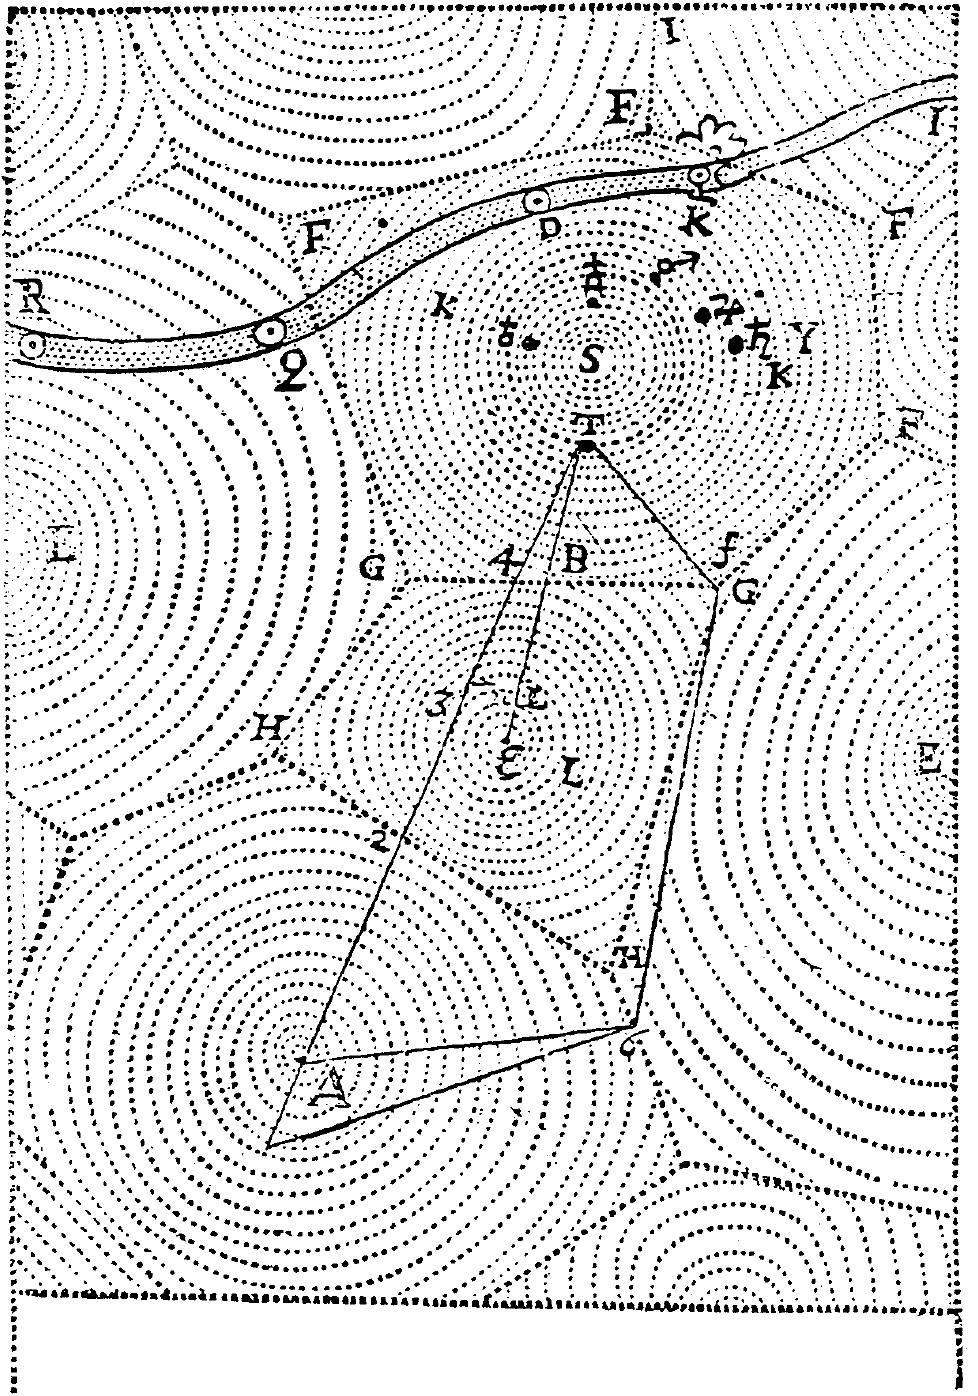
\includegraphics[width=.4\textwidth]{descartes_transparent_heavenly}
      \caption{Descartes' Heavenly Regions}
      \label{fig:descartes_heavenly}
    \end{wrapfigure}
   % ABOVE ^^^ IS THIS NOT A CONTRADICTION? Above descartes says that the higher order elements penetrate the lwoer order ones

   % The center, description of which we have delicately and deliberately escaped, is a star: a heavenly body composed entirely of the first element. The bodies which are composed of the second element and which turn about a center are called the heavens \citep[][p. 35]{descartes}. \par

   Descartes' cosmology most directly likened to a Voronoi diagram through his description of the heavens as a whole. There is a heaven (we might call it a heavenly region) for each star. \cref{fig:descartes_heavenly}, illustrates this (and provides a much better intuition of the consequences of his theory than I am able to provide in words). He writes: \say{So there are as many different heavens as there are stars, and since the number of stars is indefinite so too is the number of heavens. And the firmament is just a surface without thickness separating all the heavens from one another,}\citep[][p. 35]{descartes}.\par

   [The resemblence between Descartes' graphical representation of the heavens and the Voronoi diagram is undeniable.] The matter in the region defined as \textsc{hggh} is the heaven which rotates around $\epsilon$. Similarly, the heaven of star $S$ is precisely the matter in the region \textsc{fggf}. Perhaps more interesting, however, are the similarities between what he understands the diagram to be and the definition of a Voronoi diagram. As we mentioned earlier, Descartes believes that every star has a heaven associated with it. When we define the Voronoi diagram of a set of sites, we will note that every site has a corresponding region. The \emph{firmament}, as Descartes calls it, can be readily adapted to the Voronoi diagram with a shift in jargon: the firmament which separates the heavens from eachother are referred to as \emph{edges} in the Voronoi diagram. Should we have the desire to squint, we might even be able to glimpse an oblique reference to a Voronoi vertex: Descartes writes of the matter which lives at the intersection of three or more circles, at what appear to be \say{corners} of the firmament, it is likely smaller, and less agitated than the matter surrounding it.  
  
  % section the_world (end)
% http://www.ph.ucla.edu/epi/snow/socscimed50_923_935_2000.pdf
% https://books.google.com/books?id=cGeCNa_vookC&pg=PA152&lpg=PA152&dq=%60%60the+highest+use+of+cartography:+to+find+out+by+mapping+that+which+cannot+be+discovered+by+other+means+or,+at+least,+not+with+as+much+precision&source=bl&ots=olky0OHznK&sig=24PzRFn9l1vQWPEyMtoHx2HtZ6Y&hl=en&sa=X&ved=0ahUKEwjK6M3zop7LAhVJ-mMKHWXACD0Q6AEIHTAA#v=onepage&q=%60%60the%20highest%20use%20of%20cartography%3A%20to%20find%20out%20by%20mapping%20that%20which%20cannot%20be%20discovered%20by%20other%20means%20or%2C%20at%20least%2C%20not%20with%20as%20much%20precision&f=false
  \section{The Apocryphal Tale of John Snow} % (fold)
  \label{sec:the_apocryphal_tale_of_john_snow}
  If my dear Reader will continue to indulge, fast-forward two hundred years\ldots to 1854. It is summer in London, England. Beginning in late August, the Soho district of London experienced a cholera outbreak. The severe dehydration caused by the disease lead to dozens of deaths in a matter of days, and the numbers rose to over five hundred in the first two weeks. 

  \say{Dr. Snow's maps illustrate the highest use of cartography: to find out by mapping that which cannot be discovered by other means or, at least, not with as much precision.}
  
  % section the_apocryphal_tale_of_john_snow (end)


  \chapter*{The Voronoi Diagram}
    \addcontentsline{toc}{chapter}{The Voronoi Diagram}
    \setcounter{chapter}{2}
    \setcounter{section}{0}
	\chaptermark{The Voronoi Diagram}
	\markboth{The Voronoi Diagram}{The Voronoi Diagram}
  Suppose you are hoping to send a piece of mail via post office. In this day and age, it's uncommon to send a piece of mail, and you might ask yourself \say{Where is the nearest post office?} \par
  But why is the post office \emph{there}? \par
  To answer that question, assume the perspective of a city planner whose task is to determine where the next post office should located. The city planner might work under the assumption that people go to the post office closest to where they live. Roughly, the planner determines the areas of service for each post office, which consists of dividing the city into regions whose occupants are closer to the post office in that region than any other office. The area of service, for a particular post office, corresponds directly with the Voronoi cell of that site (the post office). We call this cell, or a region.\footnote{If the aforementioned example doesn't resonate with you, I'd encourage you to peruse \cref{appendix_one}, where I've included a plethora of other examples with the intent of motivating the problem from different perspectives, disciplines, and industries.}\par

  \section{Formalizing the Post Office Problem} % (fold)
  \label{sec:formalizing_the_post_office_problem}
  One way to understand the Voronoi diagram is via a rigorous exploration of subdivisions, manifolds, and edge algebras.\footnote{If this interests you, skip this thesis and read Guibas and Stolfi's paper.\citep{}} However,  for the purposes of this thesis we begin with a more gentle introduction. My goal is to offer a description of the Voronoi diagram that relies on its geometric properties in the Euclidian Plane. The diagram is the subdivision induced under the Voronoi assignment model, which consists in assigning every point in the plane to the site nearest to it. To construct a Voronoi diagram, we need a set of sites, $P$, and way to measure the distance between two sites, p and q, denoted $\delta(p,q)$. For the purposes of this thesis, we consider the Voronoi diagram in the plane, sites are defined as points, and the distance between any two points is the Euclidian distance.\par
  Let $P:=\{p_{1}, p_{2}, .. p_{n}\}$ a set of $n$ distinct points -- each one constituting a site -- in the plane. The Voronoi diagram of $P$ the subdivision of the plane into $n$ regions where for each region $V_{i}$ in the set of regions $V:=\{V_{1}, V_{2}, .. V_{n}\}$, $V_{i}$ is the region associated with site $p_{i}$. Further, the region $V_{i}$ is the set of points in the plane such that each point in $V_{i}$ is closer to $p_{i}$ than it is to any other site in $P$. Formally, given a plane $S$, a region or cell in a Voronoi diagram is the set of points in the plane which satisfy:
  $$V_{i} := \{\,q \in S \mid \delta(q, p_{i}) \leq \delta(q, p_{j}) \text{ for all }\, p_{j}\in P\,\text{ where }j\neq i \}.$$
  For our purposes, $S= \Re^2$, the Euclidian plane in two dimensions, and $\delta(p, q)$ is the Euclidian measure of distance in $\Re^2$. \par
  We can also think of the region $V_{i}$ as the (possibly unbounded) convex polygon which is the result of intersection of $n-1$ half-planes. Let's unpack that a little bit. Given two sites $p_{i}$ and $p_{j}$, imagine the line, $l$ connecting them. [graph] At the midpoint, $m$, of $l$, imagine a line $b$, purpendicular to $l$ and passing through $m$. Note that $b$ is the perpendicular bisector of $l$. Then $b$ splits the plane into two half-planes. Define the half-plane containing $p_{i}$ with $h(p_{i}, p_{j})$; similarly, define the half-plane containing $p_{j}$ with $h(p_{i}, p_{j})$. To connect this notion back to our first description of a Voronoi region, note that all of the points in $h(p_{i}, p_{j})$ will \emph{not} be in $p_{j}$'s region, since every point in $h(p_{i}, p_{j})$ is closer to $p_{i}$ than it is to $p_{j}$. Define set of half-planes containing $p_{i}$ as $H_{i} := \{\,h(p_{i}, p_{j}) \mid j\neq i \}$. There are $n-1$ half-planes in $H_{i}$. Consider the intersection of any two of these half-planes, $h(p_{i}, p_{j})$ and $h(p_{i}, p_{k})$. The set of points lying in the intersection of $h(p_{i}, p_{j})$ and $h(p_{i}, p_{k})$ are all of the points which are closer to $p_{i}$ than they are to $p_{j}$ or $p_{k}$. If we performed this intersection over all $n-1$ half-planes, we would have described the Voronoi region of $p_{i}$ exactly. So we can also describe the region as the intersection of a set of half-planes:
  $$V_{i} = \bigcap_{h \in H_{i}}$$ 
  Because the half-plane is a convex set\footnote{A set is convex if the line segment connecting any two points in the set is also in the region.} (or region), and the intersection of convex regions is also convex, we can say with confidence, nay, with certainty, that the Voronoi region is convex. In \cref{sec:a_naive_approach} we describe an algorithm to construct the Voronoi diagram using an approach which relies heavily on intersection of half-planes and convex regions.\par
  To summarize, every Voronoi region can be thought of as a (possibly unbounded) convex polygon whose edges are the bounding lines of the convex regions and whose vertices are the points of intersection between the bounding lines. Note that some of the edges will be line segments, while others will extend out towards infinity. We will refer to the latter type of edge as a \emph{half infinite edge}. Since the region was the result of $n-1$ half-plane intersections, we know that the region has, at most, $n-1$ edges. The Voronoi diagram of a set of sites P, $\mbox{Vor}(P)$, is the collection of all of these regions.
  We know that $\mbox{Vor}(P)$ will have $n$ regions; and we can put an upper bound on the number of edges and vertices it has by recognizing that a Voronoi diagram in $\Re^2$ is \emph{nearly} a planar graph. We make the Voronoi diagram of $P$ into a planar graph by introducing a vertex ``at infinity''. Then, we assign the vertex at infinity to be the source (or destination, when appropriate) to the half infinite edges (that is to say, all edges without two endpoints). [DIAGRAM, before and after?] \par

  Note that the size of the Voronoi graph is linear in the number of sites. \emph{Euler's Formula} states that any planar graph with $v$ vertices, $e$ edges, and $f$ faces (regions, for our purposes) the following is true:
  $v - e + f = 2.$ Applying this to $\mbox{Vor}(P)$ with an infinite vertex, which has $n$ regions, $v$ vertices, and $e$ edges we have:
  $$(v + 1) - e + n = 2.$$ Since every edge has exactly two endpoints and every (and every vertex is of degree at least 3), we can say that $2e \geq 3(v + 1)$. Together with Euler's formula, this implies that for a $n\geq 3$, the number of vertices is at most $2n -5$ and the number of edges is at most $3n -6$. 
  % section formalizing_the_post_office_problem (end)
  \section{Intersection of Half-Planes: A Na{\"i}ve Approach} % (fold)
  \label{sec:a_naive_approach}
  The structure of the planar Voronoi diagram lends itself to relatively simple algorithm for its construction. Using the notions and terminology from above, we can cobble together a naive algorithm to compute the Voronoi diagram of a set of sites. Intuitively, the Voronoi diagram of a set of sites P, $\mbox{Vor}(P)$, can be found by computing each region $V_{i}$ and defining $\mbox{Vor}(P)$ to be that set of regions. \par

  We've seen that the Voronoi region is a convex polygonal region. Futhermore, if $|P| = n$, then no region can have more than $n-1$ edges. Recall that an equivalent way of describing a Voronoi region is as the intersection of a set of half-planes. We can construct the region for a specific site by taking the intersection of this set of half-planes. Each region, then takes $\mathcal{O}(n\log n)$ time. A region needs to be computed for each of the $n$ sites, so computing the Voronoi diagram with this approach would take $\mathcal{O}(n^{2}\log n)$ time.

  [diagram?][algorithm overview for intersection fo half planes?]
  
  \section{The Voronoi Diagram and its Dual} % (fold)
  \label{sec:the_voronoi_diagram_and_its_dual}
  While the Voronoi diagram can be computed directly with relative- though certainly not always computatational- ease, it can also be computed indirectly, that is, through the construction of its dual, the \emph{Delaunay triangulation}. One of the many advantages of working with the dual is the ability to work with triangular faces instead of with polygonal regions with an unknown number of sides. Given a Voronoi diagram on $P$, $\mbox{Vor}(P)$, choose a site $p_{i} \in P$. Using $\mbox{Vor}(P)$ as a reference, draw a line connecting $p_{i}$ to the sites of the regions adjacent to it, as in \cref{fig:del_intuition1}. Do this for all the sites as in \cref{fig:del_intuition2}. If we assume that $\mbox{Vor}(P)$ contains no degeneracies, then the resulting diagram is the Delaunay Trangulation, $\mbox{Del}(P)$, as shown in \cref{fig:del_intuition}.

  \begin{figure}[!htb]
    \centering
    \begin{subtable}{.475\textwidth}
      % Define new PST objects, if not already defined
\ifx\PSTloaded\undefined
\def\PSTloaded{t}
\psset{arrowsize=.01 3.2 1.4 .3}
\psset{dotsize=.2}
\catcode`@=11

\newpsobject{PST@Border}{psline}{linewidth=.003,linestyle=solid}
\newpsobject{PST@Axes}{psline}{linewidth=.0015,linestyle=dotted,dotsep=.004}
\newpsobject{PST@Solid}{psline}{linewidth=.0015,linestyle=solid}
\newpsobject{PST@Dashed}{psline}{linewidth=.0025,linestyle=dashed,dash=.01 .01}
\newpsobject{PST@Dotted}{psline}{linewidth=.0025,linestyle=dotted,dotsep=.008}
\newpsobject{PST@LongDash}{psline}{linewidth=.0015,linestyle=dashed,dash=.02 .01}
\newpsobject{PST@Diamond}{psdots}{linewidth=.001,linestyle=solid,dotstyle=square,dotangle=45}
\newpsobject{PST@Filldiamond}{psdots}{linewidth=.001,linestyle=solid,dotstyle=square*,dotangle=45}
\newpsobject{PST@Cross}{psdots}{linewidth=.001,linestyle=solid,dotstyle=+,dotangle=45}
\newpsobject{PST@Plus}{psdots}{linewidth=.001,linestyle=solid,dotstyle=+}
\newpsobject{PST@Square}{psdots}{linewidth=.001,linestyle=solid,dotstyle=square}
\newpsobject{PST@Circle}{psdots}{linewidth=.001,linestyle=solid,dotstyle=o}
\newpsobject{PST@Triangle}{psdots}{linewidth=.001,linestyle=solid,dotstyle=triangle}
\newpsobject{PST@Pentagon}{psdots}{linewidth=.001,linestyle=solid,dotstyle=pentagon}
\newpsobject{PST@Fillsquare}{psdots}{linewidth=.001,linestyle=solid,dotstyle=square*}
\newpsobject{PST@Fillcircle}{psdots}{linewidth=.001,linestyle=solid,dotstyle=*}
\newpsobject{PST@Filltriangle}{psdots}{linewidth=.001,linestyle=solid,dotstyle=triangle*}
\newpsobject{PST@Fillpentagon}{psdots}{linewidth=.001,linestyle=solid,dotstyle=pentagon*}
\newpsobject{PST@Arrow}{psline}{linewidth=.001,linestyle=solid}
\catcode`@=12

\fi
\psset{unit=\textwidth,xunit=\textwidth,yunit=\textwidth}
\pspicture(0.000000,0.000000)(1.000000,1.000000)
\ifx\nofigs\undefined
\catcode`@=11

\PST@Border(0.3150,0.7808)
(0.3150,0.7808)
(0.5427,0.7113)

\PST@Border(0.2031,0.6088)
(0.2031,0.6088)
(0.3605,0.4149)

\PST@Border(0.7035,0.5732)
(0.7035,0.5732)
(0.9519,0.6751)

\PST@Border(0.7324,0.3287)
(0.7324,0.3287)
(0.7035,0.5732)

\PST@Border(0.5742,0.6265)
(0.5742,0.6265)
(0.7035,0.5732)

\PST@Border(0.5410,0.2304)
(0.5410,0.2304)
(0.3565,0.3639)

\PST@Border(0.3565,0.3639)
(0.3565,0.3639)
(0.3605,0.4149)

\PST@Border(0.5427,0.7113)
(0.5427,0.7113)
(0.3150,0.7808)

\PST@Border(0.2031,0.6088)
(0.2031,0.6088)
(0.0400,0.6170)

\PST@Border(0.5410,0.2304)
(0.5410,0.2304)
(0.7324,0.3287)

\PST@Border(0.3565,0.3639)
(0.3565,0.3639)
(0.5410,0.2304)

\PST@Border(0.3605,0.4149)
(0.3605,0.4149)
(0.3565,0.3639)

\PST@Border(0.5427,0.7113)
(0.5427,0.7113)
(0.6412,0.9678)

\PST@Border(0.7324,0.3287)
(0.7324,0.3287)
(0.9509,0.2326)

\PST@Border(0.3605,0.4149)
(0.3605,0.4149)
(0.2031,0.6088)

\PST@Border(0.7324,0.3287)
(0.7324,0.3287)
(0.9509,0.2326)

\PST@Border(0.5410,0.2304)
(0.5410,0.2304)
(0.5523,0.0320)

\PST@Border(0.7035,0.5732)
(0.7035,0.5732)
(0.7324,0.3287)

\PST@Border(0.5742,0.6265)
(0.5742,0.6265)
(0.5427,0.7113)

\PST@Border(0.7324,0.3287)
(0.7324,0.3287)
(0.5410,0.2304)

\PST@Border(0.3150,0.7808)
(0.3150,0.7808)
(0.2440,0.9679)

\PST@Border(0.5410,0.2304)
(0.5410,0.2304)
(0.5523,0.0320)

\PST@Border(0.2031,0.6088)
(0.2031,0.6088)
(0.0400,0.6170)

\PST@Border(0.2031,0.6088)
(0.2031,0.6088)
(0.3150,0.7808)

\PST@Border(0.5427,0.7113)
(0.5427,0.7113)
(0.6412,0.9678)

\PST@Border(0.3150,0.7808)
(0.3150,0.7808)
(0.2031,0.6088)

\PST@Border(0.7035,0.5732)
(0.7035,0.5732)
(0.5742,0.6265)

\PST@Border(0.5742,0.6265)
(0.5742,0.6265)
(0.3605,0.4149)

\PST@Border(0.3605,0.4149)
(0.3605,0.4149)
(0.5742,0.6265)

\PST@Border(0.5427,0.7113)
(0.5427,0.7113)
(0.5742,0.6265)

\PST@Border(0.3150,0.7808)
(0.3150,0.7808)
(0.2440,0.9679)

\PST@Border(0.3565,0.3639)
(0.3565,0.3639)
(0.0583,0.1580)

\PST@Border(0.7035,0.5732)
(0.7035,0.5732)
(0.9519,0.6751)

\PST@Border(0.3565,0.3639)
(0.3565,0.3639)
(0.0583,0.1580)

\PST@Dashed(0.1426,0.4554)
(0.1426,0.4554)
(0.3694,0.1336)

\PST@Dashed(0.1426,0.4554)
(0.1426,0.4554)
(0.5821,0.4217)

\PST@Dashed(0.1426,0.4554)
(0.1426,0.4554)
(0.1587,0.7674)

\PST@Dashed(0.1587,0.7674)
(0.1587,0.7674)
(0.1426,0.4554)

\PST@Dashed(0.3674,0.6343)
(0.3674,0.6343)
(0.1426,0.4554)

\PST@Dashed(0.5821,0.4217)
(0.5821,0.4217)
(0.1426,0.4554)

\PST@Dashed(0.1426,0.4554)
(0.1426,0.4554)
(0.3674,0.6343)

\PST@Dashed(0.3694,0.1336)
(0.3694,0.1336)
(0.1426,0.4554)

\PST@Fillcircle(0.1426,0.4554)
\PST@Fillcircle(0.1587,0.7674)
\PST@Fillcircle(0.4416,0.8727)
\PST@Fillcircle(0.7265,0.7654)
\PST@Fillcircle(0.8570,0.4534)
\PST@Fillcircle(0.7225,0.1534)
\PST@Fillcircle(0.3694,0.1336)
\PST@Fillcircle(0.3674,0.6343)
\PST@Fillcircle(0.5821,0.4217)
\PST@Circle(0.3150,0.7808)
\PST@Circle(0.5427,0.7113)
\PST@Circle(0.2031,0.6088)
\PST@Circle(0.5742,0.6265)
\PST@Circle(0.7035,0.5732)
\PST@Circle(0.3605,0.4149)
\PST@Circle(0.7324,0.3287)
\PST@Circle(0.3565,0.3639)
\PST@Circle(0.5410,0.2304)
\catcode`@=12
\fi
\endpspicture

      \caption{A site connected to its adjacent sites}
      \label{fig:del_intuition1}
    \end{subtable}%
    \begin{subtable}{.475\textwidth}
      \input{figs/intro/del_intuition_done.tex}
      \caption{All sites connected to their adjacent sites}
      \label{fig:del_intuition2}
    \end{subtable}
    \caption{Voronoi Diagram (Solid) and Delaunay Triangulation (Dashed)}
    \label{fig:del_intuition}
  \end{figure}

% move degenerate case to a last paragraph where you can finally be honest with them
  Note that we are being a bit cavalier with this description of the Delaunay triangulation. If four or more sites were co-circular, our result would be a Delaunay subdivision, which could be quickly modified (via the addition of edges, if necessary) to be a Delaunay triangulation. Furthermore, the Delaunay triangulation of a  Voronoi diagram whose sites are in general position is unique.\par

  Now, let's take a couple steps back and define the Delaunay triangulation a bit more rigorously, so we can better examine its properties and relation to the Voronoi diagram. It's useful, for our purposes, to consider the \emph{convex hull}.  This is the smallest convex region containing $P$, that is roughly, the intersection of all of the convex sets containing $P$. We will define this set as the smallest convex set generated by taking conbinations of points of $P$. Precisely, given points $q_{1}$,... $q_{k}$, a \emph{convex combination} of those points is defined as $\Sigma\alpha_{i}q_{i}$ where the $\alpha_{i}$'s are non-negative and $\Sigma\alpha_{i}=1.$  So, for our point set $P$ we are interested in the convex hull  $\mbox{conv}(P)$ defined as the set

   % in $\Re^2$, define $q$ to be a special type of affine combination called a \emph{convex combination}, 

  % Precisely, given $n$ points in $\Re^2$, define $q$ to be a special type of affine combination called a \emph{convex combination}, and the points generated by the combination of $p_{i}$'s are the \emph{convex set}.\cite{SHAMOS pg 90-91}
  \[
   \mbox{conv}(P) = \{\, \alpha_{1}p_{1} + ... + \alpha_{n}p_{n} \ \mid\ \text{for$ \,\alpha_{i} \in \Re, \; \alpha_{i} \geq 0$ and $\Sigma\alpha_{i} = 1$}\,\} 
  \]
  \cref{fig:convex_hull} illustrates the convex hull of the same point set used in \cref{fig:del_intuition1, fig:del_intuition2}. 
  This region of the plane is best understood in terms of a complete description of its boundary \footnote{See \cref{fig:convex_hull}}. 
  The boundary of the Delaunay triangulation of P is the convex hull of $P$. It's important to note here that every edge in the convex hull of a set of sites is an edge in the Delaunay triangulation.

  \begin{figure}[!htb]
    \centering
    
% Define new PST objects, if not already defined
\ifx\PSTloaded\undefined
\def\PSTloaded{t}
\psset{arrowsize=.01 3.2 1.4 .3}
\psset{dotsize=.2}
\catcode`@=11

\newpsobject{PST@Border}{psline}{linewidth=.003,linestyle=solid}
\newpsobject{PST@Axes}{psline}{linewidth=.0015,linestyle=dotted,dotsep=.004}
\newpsobject{PST@Solid}{psline}{linewidth=.0015,linestyle=solid}
\newpsobject{PST@Dashed}{psline}{linewidth=.0015,linestyle=dashed,dash=.01 .01}
\newpsobject{PST@Dotted}{psline}{linewidth=.0025,linestyle=dotted,dotsep=.008}
\newpsobject{PST@LongDash}{psline}{linewidth=.0015,linestyle=dashed,dash=.02 .01}
\newpsobject{PST@Diamond}{psdots}{linewidth=.001,linestyle=solid,dotstyle=square,dotangle=45}
\newpsobject{PST@Filldiamond}{psdots}{linewidth=.001,linestyle=solid,dotstyle=square*,dotangle=45}
\newpsobject{PST@Cross}{psdots}{linewidth=.001,linestyle=solid,dotstyle=+,dotangle=45}
\newpsobject{PST@Plus}{psdots}{linewidth=.001,linestyle=solid,dotstyle=+}
\newpsobject{PST@Square}{psdots}{linewidth=.001,linestyle=solid,dotstyle=square}
\newpsobject{PST@Circle}{psdots}{linewidth=.001,linestyle=solid,dotstyle=o}
\newpsobject{PST@Triangle}{psdots}{linewidth=.001,linestyle=solid,dotstyle=triangle}
\newpsobject{PST@Pentagon}{psdots}{linewidth=.001,linestyle=solid,dotstyle=pentagon}
\newpsobject{PST@Fillsquare}{psdots}{linewidth=.001,linestyle=solid,dotstyle=square*}
\newpsobject{PST@Fillcircle}{psdots}{linewidth=.001,linestyle=solid,dotstyle=*}
\newpsobject{PST@Filltriangle}{psdots}{linewidth=.001,linestyle=solid,dotstyle=triangle*}
\newpsobject{PST@Fillpentagon}{psdots}{linewidth=.001,linestyle=solid,dotstyle=pentagon*}
\newpsobject{PST@Arrow}{psline}{linewidth=.001,linestyle=solid}
\catcode`@=12

\fi
\psset{unit=2.5in,xunit=2.5in,yunit=2.5in}
\pspicture(0.000000,0.000000)(1.000000,1.000000)
\ifx\nofigs\undefined
\catcode`@=11

% .1426
% .1587
% .3694

\PST@Border(0.1426,0.4554)
(0.1426,0.4554)
(0.3694,0.1336)

% \PST@Border(0.7265,0.7654)
% (0.7265,0.7654)
% (0.8570,0.4534)

% \PST@Border(0.1587,0.7674)
% (0.1587,0.7674)
% (0.3674,0.6343)

% \PST@Border(0.1426,0.4554)
% (0.1426,0.4554)
% (0.5821,0.4217)

\PST@Border(0.3694,0.1336)
(0.3694,0.1336)
(0.7225,0.1534)

% \PST@Border(0.5821,0.4217)
% (0.5821,0.4217)
% (0.3694,0.1336)

\PST@Border(0.7225,0.1534)
(0.7225,0.1534)
(0.3694,0.1336)

\PST@Border(0.1426,0.4554)
(0.1426,0.4554)
(0.1587,0.7674)

\PST@Border(0.1587,0.7674)
(0.1587,0.7674)
(0.4416,0.8727)

% \PST@Border(0.5821,0.4217)
% (0.5821,0.4217)
% (0.8570,0.4534)

% \PST@Border(0.8570,0.4534)
% (0.8570,0.4534)
% (0.5821,0.4217)

% \PST@Border(0.5821,0.4217)
% (0.5821,0.4217)
% (0.3674,0.6343)

\PST@Border(0.1587,0.7674)
(0.1587,0.7674)
(0.1426,0.4554)

% \PST@Border(0.7225,0.1534)
% (0.7225,0.1534)
% (0.5821,0.4217)

% \PST@Border(0.3674,0.6343)
% (0.3674,0.6343)
% (0.1426,0.4554)

% \PST@Border(0.5821,0.4217)
% (0.5821,0.4217)
% (0.7265,0.7654)

% \PST@Border(0.3674,0.6343)
% (0.3674,0.6343)
% (0.4416,0.8727)

% \PST@Border(0.7265,0.7654)
% (0.7265,0.7654)
% (0.5821,0.4217)

% \PST@Border(0.3674,0.6343)
% (0.3674,0.6343)
% (0.5821,0.4217)

% \PST@Border(0.4416,0.8727)
% (0.4416,0.8727)
% (0.3674,0.6343)

\PST@Border(0.4416,0.8727)
(0.4416,0.8727)
(0.1587,0.7674)

\PST@Border(0.7225,0.1534)
(0.7225,0.1534)
(0.8570,0.4534)

\PST@Border(0.7265,0.7654)
(0.7265,0.7654)
(0.4416,0.8727)

% \PST@Border(0.3694,0.1336)
% (0.3694,0.1336)
% (0.5821,0.4217)

% \PST@Border(0.5821,0.4217)
% (0.5821,0.4217)
% (0.1426,0.4554)

% \PST@Border(0.1426,0.4554)
% (0.1426,0.4554)
% (0.3674,0.6343)

% \PST@Border(0.5821,0.4217)
% (0.5821,0.4217)
% (0.7225,0.1534)

\PST@Border(0.8570,0.4534)
(0.8570,0.4534)
(0.7225,0.1534)

% \PST@Border(0.3674,0.6343)
% (0.3674,0.6343)
% (0.1587,0.7674)

\PST@Border(0.4416,0.8727)
(0.4416,0.8727)
(0.7265,0.7654)

\PST@Border(0.8570,0.4534)
(0.8570,0.4534)
(0.7265,0.7654)

% \PST@Border(0.7265,0.7654)
% (0.7265,0.7654)
% (0.3674,0.6343)

\PST@Border(0.3694,0.1336)
(0.3694,0.1336)
(0.1426,0.4554)

% \PST@Border(0.3674,0.6343)
% (0.3674,0.6343)
% (0.7265,0.7654)

\PST@Fillcircle(0.1426,0.4554)
\PST@Fillcircle(0.1587,0.7674)
\PST@Fillcircle(0.4416,0.8727)
\PST@Fillcircle(0.7265,0.7654)
\PST@Fillcircle(0.8570,0.4534)
\PST@Fillcircle(0.7225,0.1534)
\PST@Fillcircle(0.3694,0.1336)
\PST@Fillcircle(0.3674,0.6343)
\PST@Fillcircle(0.5821,0.4217)

\catcode`@=12
\fi
\endpspicture

      % \caption{All sites connected to their adjacent sites}
    \caption{Convex hull of a set of points}
    \label{fig:convex_hull}
  \end{figure}

  What distinguishes the Delaunay triangulation of a set $P$ from any other triangulation of $P$ are its unique properties, which are directly related to its privileged position as the dual of the Voronoi diagram. (maximizes the minimum angle of all triangulations and why this is cool, empty circumcircle property for each facet)(also, do I need to provide a proof that the straight line dual of the voronoi is a triangulation?)

  As a side note, this is precisely how we confirm the delaunayhood of a subdivision. More precisely, if every face (triangle) in the diagram is \emph{locally delaunay} (that is to say, passes the circle test), then the diagram is considered to be \emph{globally delaunay}.


  % section the_voronoi_diagram_and_its_dual (end)
  \section{Applications of Voronoi and Delaunay Diagrams} % (fold)
  \label{sec:applications_of_voronoi_and_delaunay_diagrams}
  Beyond the intrinsic allure of the Voronoi diagram and its stright line dual, the Delaunay triangulation, lies a fascinating set of linear time reductions to some of the central proximity problems. This means that if we take the time to preprocess a set of sites into a Voronoi diagram, then we can answer many different questions in linear (or better!) time. This is especially significant when the time complexity of answering that question is greater than $\mathcal{O}(n)$.\par 

  From the previous section \cref{sec:the_voronoi_diagram_and_its_dual}, we saw that it is possible to obtain the dual of the Voronoi diagram in linear time. Thus, we can use the Voronoi diagram to solve the problem of triangulating a set of sites $P$, by returning the dual of the diagram. 

  The Post Office Problem is a classic, though perhaps slightly dated, motivation for the Voronoi diagram. However, it captures one of the central use cases for the Voronoi diagram, which is its ability to answer the \emph{nearest neighbor problem}. The nearest neighbor problem can be stated as such: given a set of sites $P$, and a query point $q$, return the point in $P$ which is closest to $q$. Recall that the Voronoi diagram partitions the plane into a set of $\mid\,P\,\mid$ regions which satisfy the stipulation that every point in a given region is closer to the site associated with that region than it is to any other site. Then, given a query point $q$ and a Voronoi diagram of $P$, we can answer the nearest neighbor question by simply locating the region that $q$ is in, a question we can answer in $\mathcal{O}(\log n)$ time with linear auxilliary storage.\citep{shamos, p 214}\par
  
  (Closely) related to this are the \emph{closest pair} and \emph{all nearest neighbors} problems. The closest pair problem asks, given a set of sites $P$, which pair of points $p_{i}$ and $p_{j}$ in $P$ are closest? The all nearest neighbors problem can be framed similarly: given a set of sites $P$, return a collection of pairs ($p_{i}$, $p_{j}$) such that $p_{j}$ is the nearest neighbor of $p_{i}$.\footnote{Note here that the closest pair problem is really a specification of the nearest neighbors problem where the query point $q$ is some $p_{i}$ in $P$ and not arbitrary $q$ in $\Re^2$.} When given a Voronoi diagram on those sites, the all nearest neighbors problem can be answered in linear time by recognizing that the nearest neighbor of a single site must be one of the sites with which it shares an edge. Equivalently, we can consider the Delaunay triangulation on the same set of sites, $\mbox{Del}(P)$. Recall that each vertex on the Delaunay triangulation is a site of $\mbox{Vor}(P)$. Furthermore, note that the line segment connecting a vertex $p_{i}$ of $\mbox{Del}(P)$ to its nearest neighbor is, and must be, one of the edges in $\mbox{Del}(P)$. So, if we spend time on the order of $\mathcal{O}(n)$ computing the result of the all nearest neighbors problem on $\mbox{Vor}(P)$, we will, by definition, have the answer the the closest pair problem for each site in $P$. 

  [MINIMUM SPANNING TREE, other problems?]
  
  \section{Properties of Voronoi and Delaunay Diagrams} % (fold)
  \label{sec:properties_of_voronoi_and_delaunay_diagrams}
  This section summarizes the terminology from \cref{sec:formalizing_the_post_office_problem, sec:a_naive_approach, sec:the_voronoi_diagram_and_its_dual, sec:applications_of_voronoi_and_delaunay_diagrams} 
  
  % section properties_of_voronoi_and_delaunay_diagrams (end)

  % section applications_of_voronoi_and_delaunay_diagrams (end)
  \section{Statement of algorithm goals (High Performance Computing)} % (fold)
  \label{sec:statement_of_algorithm_goals_high_performance_computing_}
    In this thesis, we wish to bear witness to the effects of modifying the two aspects of two different approaches to constructing the Voronoi diagram (or the Delaunay triangulation). Further, we ask the following question, which will be further motivated by the section on divide and conquer algorithms: ``given two valid delaunay triangulations (or voronoi diagrams), merge them''. So we're trying to merge them in parallel so we can see the results and maybe say something about that. We're also thinking about the question ``is there a way to \emph{order} the randomized incremental approach in a way that allows us to have multiple workers attacking the problem while also minimizing the amount of conflict?'' And we'll see more information on that problem in the section on randomized incremental and also the section on progress with that endeavor.]
  % section statement_of_algorithm_goals_high_performance_computing_ (end)

  \chapter*{Constructing the Voronoi Diagram}
    \addcontentsline{toc}{chapter}{Constructing the Voronoi Diagram}
    \chaptermark{Constructing the Voronoi Diagram}
    \markboth{Constructing the Voronoi Diagram}{Constructing the Voronoi Diagram}
    \setcounter{chapter}{3}
    \setcounter{section}{0}
  In \cref{sec:formalizing_the_post_office_problem} we saw a naive algorithm for computing the Voronoi diagram of a set of $n$ sites. The time complexity of the half-plane intersection algorithm, as we discovered in \cref{sec:a_naive_approach}, is $\mathcal{O}(n^{2}\log n)$. Though it provides an intuition of the diagram, there are far more optimal approaches to the construction of the Voronoi diagram. They fall into three rough categories: incremental approaches, divide and conquer approaches, and sweepline approaches. The worst case time complexity for each of these is $\mathcal{O}(n^{2})$, $\mathcal{O}(n\log n)$ and $\mathcal{O}(n\log n)$ respectively. In this chapter, we will examine two classic algorithsm to compute the Voronoi diagram: a divide and conquer algorithm, presented by Guibas and Stolfi [ref]; and Steven Fortune's sweepline algorithm. \par
  
  As it turns out, we can't do better than $\mathcal{O}(n\log n)$. Curious reader that you are, you might wonder: \say{Why?} And the answer is this: we can show, quite easily, in fact, that the problem of sorting numbers is \emph{reducible} to the problem of computing the Voronoi diagram. This means that given a set of integers, we can use an algorithm to construct of Voronoi diagram as a subroutine to compute the sorted set. Furthermore, it implies that we will never be able to construct the Voronoi diagram faster (in terms of complexity) than we will be able to sort integers. Thus, an immediate consequence of this reduction is a tight bound on the Voronoi diagram; it can be constructed in optimal time $\theta(n\log n)$. (Cool fact: Asymptotically, the complexity of the constructing the diagram is no more difficult than the task of finding a region.)\par
  
  % subsection constructing_a_voronoi_region (end)
  % section a_naive_approach (end)

  \section{Fortune's Algorithm: A Sweepline Approach} % (fold)
  \label{sec:fortune_s_algorithm}
  In the 1980's Steven Fortune proposed a sweepline algorithm with asymptotic running time $\mathcal{O}(n\log n)$ and using $\mathcal{O}(n)$ space. Fortune's algorithm makes use of a sweepline, a horizontal line beginning at the top of the plane and descending to the bottom of the plane. The general strategy of the algorithm is to use a line to scan the plane, updating information about the structure of the diagram whenever the sweepline intersects a point of interest. Some of these points of interest are known in advance, and others arise during the construction of the diagram. With a bit of planning and the clever choice of a quad-edge data structure, the task of constructing the Voronoi diagram with this approach immediately yields its dual, the Delaunay triangulation. [ref guibas]

  \subsection{Conceptual Overview} % (fold)
  \label{sub:conceptual_overview}
  Fortune's algorithm uses a few key concepts and structures to support the construction of the Voronoi diagram. To gain an understanding of how to algorithm works, it's easiest to apply it to a set of sites. Let $P:=\{p_{1}, p_{2}, .. p_{n}\}$ be the a set of $n$ distinct points in $\Re^{2}$. Then, define the sweepline $s$ to be a horizontal line in $\Re^{2}$. Note that conceptually, $s$ begins at the ``top'' of the plane, but in practice, it is sufficient that $s$ be initialized with a y-coordinate greater than the site with the largest y-coordinate.\par

  An astute reader might wonder how exactly we construct the Voronoi diagram with nothing but a set of sites and a vague notion of a line that falls down the plane. After all, there's no obvious method by which the intersection of the sweepline with a point of interest might yield a Voronoi vertex or edge. Further, it would seem that even if we could provide such a relationship would be subject to change as soon as the sweepline encountered the next point of interest. \par
  Herein lies the elegance of Fortune's algorithm. Consider the portion of the plane that the sweepline has already encountered, this portion constitutes a closed half-plane, $s^+$. If a site exists in $s^+$, then any point $q$ in $s^+$ which is closer to that site than it is to $s$ will not be assigned to a site below $s$. When the sweepline $s$ encounters a site $p_{i}$ we call this a \emph{site event}. We consider the locus of points which are closer to $p_{i}$ than to $s$. The set of points equidistant to $s$ and $p_{i}$ form a parabolic arc. This arc, denoted $\beta_{i}$, is added to a a sequence of parabolic arcs called the \emph{beachfront}. We will refer to the beachfront as $\beta(P)$. The crucial observation is that the points above $\beta(P)$ will be assigned to a site already encountered by $s$. \par

  [Make sure there's a clear difference between the notation used for the parabola and the notation used for an arc].
  To understand how the beachfront plays a role in constructing the Voronoi diagram, let's consider times where the structure of the beachfront changes. New arcs are added to the beachfront whenever a site event occurs. At the moment where the new arc, $\beta_{i}$, is inserted into the beachfront, it is a simple vertical line (or a parabola of no width). If there is an arc above $\beta_{i}$, $\beta_{i}$ will only intersect it at one point since the beachfront is x-monotone. To insert $\beta_{i}$ into the beachfront, we split the arc above it into two parabolic arcs and insert $\beta_{i}$ in between the split arcs. We record the points where $\beta_{i}$ intersects with the arcs adjacent to it, and we refer to these points as \emph{breakpoints}\footnote{Note that this means that the right breakpoint of $\beta_{i}$ is the same as the left breakpoint of the arc which is adjacent on the right. Similarly, the right breakpoint of the arc adjacent to $\beta_{i}$ on the left is equal to $\beta_{i}$'s left breakpoint.} As $s$ moves downward, the breakpoints of each arc in the beachfront $\beta(P)$ change since the parabola that governs the arc widens. Another way to understand this is to recognize that that parabola whose corresponding arc is $\beta_{i}$ has as its focus the site $p_{i}$ and $s$ as its directrix. If we were to draw lines that tracked the movement of the breakpoints for the beachfront as the sweepline descended, they would each trace out the Voronoi edges. So we know that arcs get added to the beachfront whenever a site event occurs, in fact, the \emph{only} time an arc gets added to the beachfront is when a site event occurs. [And we can prove that!] \par

    \begin{figure}[!htb]
      \centering
      \begin{subtable}{0.475\textwidth}
        \centering
        % GNUPLOT: LaTeX picture using PSTRICKS macros
% Define new PST objects, if not already defined
\ifx\PSTloaded\undefined
\def\PSTloaded{t}
\psset{arrowsize=.01 3.2 1.4 .3}
\psset{dotsize=.2}
\catcode`@=11

\newpsobject{PST@Border}{psline}{linewidth=.002,linestyle=solid}
\newpsobject{PST@ThickBorder}{psline}{linewidth=.003,linestyle=solid}
\newpsobject{PST@Axes}{psline}{linewidth=.0015,linestyle=dotted,dotsep=.004}
\newpsobject{PST@Solid}{psline}{linewidth=.0015,linestyle=solid}
\newpsobject{PST@Dashed}{psline}{linewidth=.0015,linestyle=dashed,dash=.01 .01}
\newpsobject{PST@Dotted}{psline}{linewidth=.0025,linestyle=dotted,dotsep=.008}
\newpsobject{PST@LongDash}{psline}{linewidth=.0015,linestyle=dashed,dash=.02 .01}
\newpsobject{PST@Diamond}{psdots}{linewidth=.001,linestyle=solid,dotstyle=square,dotangle=45}
\newpsobject{PST@Filldiamond}{psdots}{linewidth=.001,linestyle=solid,dotstyle=square*,dotangle=45}
\newpsobject{PST@Cross}{psdots}{linewidth=.001,linestyle=solid,dotstyle=+,dotangle=45}
\newpsobject{PST@Plus}{psdots}{linewidth=.001,linestyle=solid,dotstyle=+}
\newpsobject{PST@Square}{psdots}{linewidth=.001,linestyle=solid,dotstyle=square}
\newpsobject{PST@Circle}{psdots}{linewidth=.001,linestyle=solid,dotstyle=o}
\newpsobject{PST@Triangle}{psdots}{linewidth=.001,linestyle=solid,dotstyle=triangle}
\newpsobject{PST@Pentagon}{psdots}{linewidth=.001,linestyle=solid,dotstyle=pentagon}
\newpsobject{PST@Fillsquare}{psdots}{linewidth=.001,linestyle=solid,dotstyle=square*}
\newpsobject{PST@Fillcircle}{psdots}{linewidth=.001,linestyle=solid,dotstyle=*}
\newpsobject{PST@Filltriangle}{psdots}{linewidth=.001,linestyle=solid,dotstyle=triangle*}
\newpsobject{PST@Fillpentagon}{psdots}{linewidth=.001,linestyle=solid,dotstyle=pentagon*}
\newpsobject{PST@Arrow}{psline}{linewidth=.001,linestyle=solid}
\catcode`@=12

\fi
\psset{unit=2.5in,xunit=2.5in,yunit=2.5in}
\pspicture(0.000000,0.250000)(1.000000,1.000000)
\ifx\nofigs\undefined
\catcode`@=11

\rput[l](0.47,0.95){\scriptsize{$\alpha$}}
\PST@ThickBorder(0.5237,0.9679)
(0.5247,0.9627)
(0.5273,0.9499)
(0.5299,0.9376)
(0.5326,0.9258)
(0.5352,0.9146)
(0.5378,0.9039)
(0.5404,0.8937)
(0.5430,0.8841)
(0.5456,0.8751)
(0.5482,0.8665)
(0.5508,0.8585)
(0.5534,0.8511)
(0.5560,0.8442)
(0.5586,0.8378)
(0.5612,0.8320)
(0.5638,0.8267)
(0.5664,0.8219)
(0.5690,0.8177)
(0.5716,0.8141)
(0.5742,0.8109)
(0.5768,0.8083)
(0.5794,0.8063)
(0.5821,0.8048)
(0.5847,0.8038)
(0.5873,0.8034)
(0.5899,0.8035)
(0.5925,0.8041)
(0.5951,0.8053)
(0.5977,0.8070)
(0.6003,0.8093)
(0.6029,0.8121)
(0.6055,0.8154)
(0.6081,0.8193)
(0.6107,0.8237)
(0.6133,0.8287)
(0.6159,0.8342)
(0.6185,0.8403)
(0.6211,0.8468)
(0.6237,0.8540)
(0.6263,0.8616)
(0.6290,0.8698)
(0.6316,0.8786)
(0.6342,0.8878)
(0.6368,0.8977)
(0.6394,0.9080)
(0.6420,0.9189)
(0.6446,0.9304)
(0.6472,0.9423)
(0.6498,0.9548)
(0.6524,0.9679)

\rput[l](0.0450,0.770){\scriptsize{\emph{s}}}
\PST@Border(0.0400,0.7983)
(0.0400,0.7983)
(0.0726,0.7983)
(0.1051,0.7983)
(0.1377,0.7983)
(0.1703,0.7983)
(0.2028,0.7983)
(0.2354,0.7983)
(0.2680,0.7983)
(0.3005,0.7983)
(0.3331,0.7983)
(0.3657,0.7983)
(0.3982,0.7983)
(0.4308,0.7983)
(0.4634,0.7983)
(0.4960,0.7983)
(0.5285,0.7983)
(0.5611,0.7983)
(0.5937,0.7983)
(0.6262,0.7983)
(0.6588,0.7983)
(0.6914,0.7983)
(0.7239,0.7983)
(0.7565,0.7983)
(0.7891,0.7983)
(0.8216,0.7983)
(0.8542,0.7983)
(0.8868,0.7983)
(0.9193,0.7983)
(0.9519,0.7983)

\rput[l](0.22,0.4840){\scriptsize{$p_{i}$}}
\PST@Fillcircle(0.1911,0.4840)

\rput[l](0.56,0.85){\scriptsize{$p_{j}$}}
\PST@Fillcircle(0.5881,0.8084)

\rput[l](0.80,0.6485){\scriptsize{$p_{k}$}}
\PST@Fillcircle(0.8781,0.6485)
\catcode`@=12
\fi
\endpspicture

        \caption{Handling a Site Event}
        \label{fig:fortune_0}
      \end{subtable}%
      \begin{subtable}{0.475\textwidth}
        \centering
        % GNUPLOT: LaTeX picture using PSTRICKS macros
% Define new PST objects, if not already defined
\ifx\PSTloaded\undefined
\def\PSTloaded{t}
\psset{arrowsize=.01 3.2 1.4 .3}
\psset{dotsize=.2}
\catcode`@=11

\newpsobject{PST@Border}{psline}{linewidth=.002,linestyle=solid}
\newpsobject{PST@ThickBorder}{psline}{linewidth=.003,linestyle=solid}
\newpsobject{PST@Axes}{psline}{linewidth=.0015,linestyle=dotted,dotsep=.004}
\newpsobject{PST@Solid}{psline}{linewidth=.0015,linestyle=solid}
\newpsobject{PST@Dashed}{psline}{linewidth=.0015,linestyle=dashed,dash=.01 .01}
\newpsobject{PST@Dotted}{psline}{linewidth=.0025,linestyle=dotted,dotsep=.008}
\newpsobject{PST@LongDash}{psline}{linewidth=.0015,linestyle=dashed,dash=.02 .01}
\newpsobject{PST@Diamond}{psdots}{linewidth=.001,linestyle=solid,dotstyle=square,dotangle=45}
\newpsobject{PST@Filldiamond}{psdots}{linewidth=.001,linestyle=solid,dotstyle=square*,dotangle=45}
\newpsobject{PST@Cross}{psdots}{linewidth=.001,linestyle=solid,dotstyle=+,dotangle=45}
\newpsobject{PST@Plus}{psdots}{linewidth=.001,linestyle=solid,dotstyle=+}
\newpsobject{PST@Square}{psdots}{linewidth=.001,linestyle=solid,dotstyle=square}
\newpsobject{PST@Circle}{psdots}{linewidth=.001,linestyle=solid,dotstyle=o}
\newpsobject{PST@Triangle}{psdots}{linewidth=.001,linestyle=solid,dotstyle=triangle}
\newpsobject{PST@Pentagon}{psdots}{linewidth=.001,linestyle=solid,dotstyle=pentagon}
\newpsobject{PST@Fillsquare}{psdots}{linewidth=.001,linestyle=solid,dotstyle=square*}
\newpsobject{PST@Fillcircle}{psdots}{linewidth=.001,linestyle=solid,dotstyle=*}
\newpsobject{PST@Filltriangle}{psdots}{linewidth=.001,linestyle=solid,dotstyle=triangle*}
\newpsobject{PST@Fillpentagon}{psdots}{linewidth=.001,linestyle=solid,dotstyle=pentagon*}
\newpsobject{PST@Arrow}{psline}{linewidth=.001,linestyle=solid}
\catcode`@=12

\fi
\psset{unit=2.5in,xunit=2.5in,yunit=2.5in}
\pspicture(0.000000,0.250000)(1.000000,1.000000)
\ifx\nofigs\undefined
\catcode`@=11

\rput[l](0.23,0.94){\scriptsize{$\alpha$}}
\PST@ThickBorder(0.2702,0.9679)
(0.2716,0.9658)
(0.2742,0.9618)
(0.2768,0.9579)
(0.2794,0.9540)
(0.2820,0.9502)
(0.2846,0.9463)
(0.2872,0.9425)
(0.2898,0.9388)
(0.2924,0.9351)
(0.2950,0.9314)
(0.2976,0.9277)
(0.3002,0.9241)
(0.3028,0.9205)
(0.3055,0.9169)
(0.3081,0.9134)
(0.3107,0.9099)
(0.3133,0.9064)
(0.3159,0.9030)
(0.3185,0.8996)
(0.3211,0.8963)
(0.3237,0.8929)
(0.3263,0.8896)
(0.3289,0.8864)
(0.3315,0.8831)
(0.3341,0.8799)
(0.3367,0.8767)
(0.3393,0.8736)
(0.3419,0.8705)
(0.3445,0.8674)
(0.3471,0.8644)
(0.3497,0.8614)
(0.3524,0.8584)
(0.3550,0.8555)
(0.3576,0.8526)
(0.3602,0.8497)
(0.3628,0.8468)
(0.3654,0.8440)
(0.3680,0.8413)
(0.3706,0.8385)
(0.3732,0.8358)
(0.3758,0.8331)
(0.3784,0.8305)
(0.3810,0.8279)
(0.3836,0.8253)
(0.3862,0.8227)
(0.3888,0.8202)
(0.3914,0.8177)
(0.3940,0.8153)
(0.3966,0.8129)
(0.3992,0.8105)
(0.4019,0.8081)
(0.4045,0.8058)
(0.4071,0.8035)
(0.4097,0.8013)
(0.4123,0.7991)
(0.4149,0.7969)
(0.4175,0.7947)
(0.4201,0.7926)
(0.4227,0.7905)
(0.4253,0.7884)
(0.4279,0.7864)
(0.4305,0.7844)
(0.4331,0.7825)
(0.4357,0.7805)
(0.4383,0.7786)
(0.4409,0.7768)
(0.4435,0.7749)
(0.4461,0.7731)
(0.4488,0.7714)
(0.4514,0.7697)
(0.4540,0.7680)
(0.4566,0.7663)
(0.4592,0.7647)
(0.4618,0.7631)
(0.4644,0.7615)
(0.4670,0.7600)
(0.4696,0.7584)
(0.4722,0.7570)
(0.4748,0.7555)
(0.4774,0.7541)
(0.4800,0.7528)
(0.4826,0.7514)
(0.4852,0.7501)
(0.4878,0.7488)
(0.4904,0.7476)
(0.4930,0.7464)
(0.4957,0.7452)
(0.4983,0.7441)
(0.5009,0.7430)
(0.5035,0.7419)
(0.5061,0.7408)
(0.5087,0.7398)
(0.5113,0.7389)
(0.5139,0.7379)
(0.5165,0.7370)
(0.5191,0.7361)
(0.5217,0.7353)
(0.5243,0.7344)
(0.5269,0.7337)
(0.5295,0.7329)
\PST@ThickBorder(0.5295,0.7329)
(0.5321,0.7322)
(0.5347,0.7315)
(0.5373,0.7309)
(0.5399,0.7302)
(0.5425,0.7297)
(0.5452,0.7291)
(0.5478,0.7286)
(0.5504,0.7281)
(0.5530,0.7276)
(0.5556,0.7272)
(0.5582,0.7268)
(0.5608,0.7265)
(0.5634,0.7261)
(0.5660,0.7258)
(0.5686,0.7256)
(0.5712,0.7253)
(0.5738,0.7252)
(0.5764,0.7250)
(0.5790,0.7249)
(0.5816,0.7248)
(0.5842,0.7247)
(0.5868,0.7247)
(0.5894,0.7247)
(0.5921,0.7247)
(0.5947,0.7248)
(0.5973,0.7249)
(0.5999,0.7250)
(0.6025,0.7252)
(0.6051,0.7254)
(0.6077,0.7256)
(0.6103,0.7259)
(0.6129,0.7262)
(0.6155,0.7265)
(0.6181,0.7268)
(0.6207,0.7272)
(0.6233,0.7277)
(0.6259,0.7281)
(0.6285,0.7286)
(0.6311,0.7291)
(0.6337,0.7297)
(0.6363,0.7303)
(0.6389,0.7309)
(0.6416,0.7316)
(0.6442,0.7322)
(0.6468,0.7330)
(0.6494,0.7337)
(0.6520,0.7345)
(0.6546,0.7353)
(0.6572,0.7362)
(0.6598,0.7371)
(0.6624,0.7380)
(0.6650,0.7389)
(0.6676,0.7399)
(0.6702,0.7409)
(0.6728,0.7420)
(0.6754,0.7430)
(0.6780,0.7442)
(0.6806,0.7453)
(0.6832,0.7465)
(0.6858,0.7477)
(0.6885,0.7489)
(0.6911,0.7502)
(0.6937,0.7515)
(0.6963,0.7529)
(0.6989,0.7542)
(0.7015,0.7556)
(0.7041,0.7571)
(0.7067,0.7585)
(0.7093,0.7601)
(0.7119,0.7616)
(0.7145,0.7632)
(0.7171,0.7648)
(0.7197,0.7664)
(0.7223,0.7681)
(0.7249,0.7698)
(0.7275,0.7715)
(0.7301,0.7733)
(0.7327,0.7751)
(0.7353,0.7769)
(0.7380,0.7788)
(0.7406,0.7807)
(0.7432,0.7826)
(0.7458,0.7845)
(0.7484,0.7865)
(0.7510,0.7886)
(0.7536,0.7906)
(0.7562,0.7927)
(0.7588,0.7949)
(0.7614,0.7970)
(0.7640,0.7992)
(0.7666,0.8014)
(0.7692,0.8037)
(0.7718,0.8060)
(0.7744,0.8083)
(0.7770,0.8106)
(0.7796,0.8130)
(0.7822,0.8155)
(0.7849,0.8179)
(0.7875,0.8204)
(0.7901,0.8229)
\PST@ThickBorder(0.7901,0.8229)
(0.7927,0.8255)
(0.7953,0.8280)
(0.7979,0.8307)
(0.8005,0.8333)
(0.8031,0.8360)
(0.8057,0.8387)
(0.8083,0.8414)
(0.8109,0.8442)
(0.8135,0.8470)
(0.8161,0.8499)

\rput[l](0.895,0.91){\scriptsize{$\omega$}}
\PST@LongDash(0.8161,0.8499)
(0.8161,0.8499)
(0.8187,0.8330)
(0.8213,0.8168)
(0.8239,0.8014)
(0.8266,0.7867)
(0.8292,0.7727)
(0.8318,0.7594)
(0.8344,0.7469)
(0.8370,0.7351)
(0.8396,0.7240)
(0.8422,0.7136)
(0.8448,0.7040)
(0.8474,0.6951)
(0.8500,0.6869)
(0.8526,0.6794)
(0.8552,0.6727)
(0.8578,0.6667)
(0.8604,0.6614)
(0.8630,0.6568)
(0.8656,0.6530)
(0.8682,0.6499)
(0.8708,0.6475)
(0.8735,0.6459)
(0.8761,0.6449)
(0.8787,0.6447)
(0.8813,0.6452)
(0.8839,0.6465)
(0.8865,0.6484)
(0.8891,0.6511)
(0.8917,0.6545)
(0.8943,0.6587)
(0.8969,0.6635)
(0.8995,0.6691)
(0.9021,0.6755)
(0.9047,0.6825)
(0.9073,0.6903)
(0.9099,0.6988)
(0.9125,0.7080)
(0.9151,0.7179)
(0.9177,0.7286)
(0.9203,0.7400)
(0.9230,0.7521)
(0.9256,0.7649)
(0.9282,0.7785)
(0.9308,0.7928)
(0.9334,0.8078)
(0.9360,0.8236)
(0.9386,0.8400)
(0.9412,0.8572)
(0.9438,0.8751)
(0.9464,0.8938)
(0.9490,0.9131)
(0.9516,0.9332)
(0.9519,0.9355)

\PST@Border(0.0400,0.6409)
(0.0400,0.6409)
(0.0726,0.6409)
(0.1051,0.6409)
(0.1377,0.6409)
(0.1703,0.6409)
(0.2028,0.6409)
(0.2354,0.6409)
(0.2680,0.6409)
(0.3005,0.6409)
(0.3331,0.6409)
(0.3657,0.6409)
(0.3982,0.6409)
(0.4308,0.6409)
(0.4634,0.6409)
(0.4960,0.6409)
(0.5285,0.6409)
(0.5611,0.6409)
(0.5937,0.6409)
(0.6262,0.6409)
(0.6588,0.6409)
(0.6914,0.6409)
(0.7239,0.6409)
(0.7565,0.6409)
(0.7891,0.6409)
(0.8216,0.6409)
(0.8542,0.6409)
(0.8868,0.6409)
(0.9193,0.6409)
(0.9519,0.6409)

\PST@Fillcircle(0.1911,0.4840)
\PST@Fillcircle(0.5881,0.8084)
\PST@Fillcircle(0.8781,0.6485)
\catcode`@=12
\fi
\endpspicture

        \caption{Adding an arc to the beachfront}
        \label{fig:fortune_1}
      \end{subtable}
      \begin{subtable}{0.475\textwidth}
        \centering
        \input{figs/ch1/fortune/ex1_p2.tex}
        \caption{Add a new Circle Event}
        \label{fig:fortune_2}
      \end{subtable}
      \begin{subtable}{0.475\textwidth}
        \centering
        % GNUPLOT: LaTeX picture using PSTRICKS macros
% Define new PST objects, if not already defined
\ifx\PSTloaded\undefined
\def\PSTloaded{t}
\psset{arrowsize=.01 3.2 1.4 .3}
\psset{dotsize=.2}
\catcode`@=11

\newpsobject{PST@Border}{psline}{linewidth=.002,linestyle=solid}
\newpsobject{PST@ThickBorder}{psline}{linewidth=.003,linestyle=solid}
\newpsobject{PST@VeryThickBorder}{psline}{linewidth=.008,linestyle=solid}
\newpsobject{PST@Axes}{psline}{linewidth=.0015,linestyle=dotted,dotsep=.004}
\newpsobject{PST@Solid}{psline}{linewidth=.0015,linestyle=solid}
\newpsobject{PST@Dashed}{psline}{linewidth=.0015,linestyle=dashed,dash=.01 .01}
\newpsobject{PST@Dotted}{psline}{linewidth=.0025,linestyle=dotted,dotsep=.008}
\newpsobject{PST@LongDash}{psline}{linewidth=.0015,linestyle=dashed,dash=.02 .01}
\newpsobject{PST@Diamond}{psdots}{linewidth=.001,linestyle=solid,dotstyle=square,dotangle=45}
\newpsobject{PST@Filldiamond}{psdots}{linewidth=.001,linestyle=solid,dotstyle=square*,dotangle=45}
\newpsobject{PST@Cross}{psdots}{linewidth=.001,linestyle=solid,dotstyle=+,dotangle=45}
\newpsobject{PST@Plus}{psdots}{linewidth=.001,linestyle=solid,dotstyle=+}
\newpsobject{PST@Square}{psdots}{linewidth=.001,linestyle=solid,dotstyle=square}
\newpsobject{PST@Circle}{psdots}{linewidth=.001,linestyle=solid,dotstyle=o}
\newpsobject{PST@Triangle}{psdots}{linewidth=.001,linestyle=solid,dotstyle=triangle}
\newpsobject{PST@Pentagon}{psdots}{linewidth=.001,linestyle=solid,dotstyle=pentagon}
\newpsobject{PST@Fillsquare}{psdots}{linewidth=.001,linestyle=solid,dotstyle=square*}
\newpsobject{PST@Fillcircle}{psdots}{linewidth=.001,linestyle=solid,dotstyle=*}
\newpsobject{PST@Filltriangle}{psdots}{linewidth=.001,linestyle=solid,dotstyle=triangle*}
\newpsobject{PST@Fillpentagon}{psdots}{linewidth=.001,linestyle=solid,dotstyle=pentagon*}
\newpsobject{PST@Arrow}{psline}{linewidth=.001,linestyle=solid}
\catcode`@=12

\fi
\psset{unit=\textwidth,xunit=\textwidth,yunit=\textwidth}
\pspicture(0.000000,0.0000)(1.000000,1.000000)
\ifx\nofigs\undefined
\catcode`@=11



\rput[t](0.35,0.5){$\gamma$}
\psline(0.0400,0.4288)
(0.0415,0.4279)
(0.0441,0.4264)
(0.0467,0.4249)
(0.0493,0.4234)
(0.0519,0.4219)
(0.0545,0.4205)
(0.0571,0.4191)
(0.0597,0.4177)
(0.0624,0.4163)
(0.0650,0.4150)
(0.0676,0.4137)
(0.0702,0.4124)
(0.0728,0.4112)
(0.0754,0.4100)
(0.0780,0.4088)
(0.0806,0.4076)
(0.0832,0.4065)
(0.0858,0.4053)
(0.0884,0.4043)
(0.0910,0.4032)
(0.0936,0.4022)
(0.0962,0.4012)
(0.0988,0.4002)
(0.1014,0.3992)
(0.1040,0.3983)
(0.1066,0.3974)
(0.1092,0.3966)
(0.1119,0.3957)
(0.1145,0.3949)
(0.1171,0.3941)
(0.1197,0.3934)
(0.1223,0.3926)
(0.1249,0.3919)
(0.1275,0.3913)
(0.1301,0.3906)
(0.1327,0.3900)
(0.1353,0.3894)
(0.1379,0.3888)
(0.1405,0.3883)
(0.1431,0.3878)
(0.1457,0.3873)
(0.1483,0.3868)
(0.1509,0.3864)
(0.1535,0.3860)
(0.1561,0.3856)
(0.1588,0.3853)
(0.1614,0.3849)
(0.1640,0.3846)
(0.1666,0.3844)
(0.1692,0.3841)
(0.1718,0.3839)
(0.1744,0.3837)
(0.1770,0.3836)
(0.1796,0.3834)
(0.1822,0.3833)
(0.1848,0.3832)
(0.1874,0.3832)
(0.1900,0.3832)
(0.1926,0.3832)
(0.1952,0.3832)
(0.1978,0.3832)
(0.2004,0.3833)
(0.2030,0.3834)
(0.2056,0.3836)
(0.2083,0.3837)
(0.2109,0.3839)
(0.2135,0.3842)
(0.2161,0.3844)
(0.2187,0.3847)
(0.2213,0.3850)
(0.2239,0.3853)
(0.2265,0.3857)
(0.2291,0.3860)
(0.2317,0.3864)
(0.2343,0.3869)
(0.2369,0.3873)
(0.2395,0.3878)
(0.2421,0.3884)
(0.2447,0.3889)
(0.2473,0.3895)
(0.2499,0.3901)
(0.2525,0.3907)
(0.2552,0.3914)
(0.2578,0.3920)
(0.2604,0.3927)
(0.2630,0.3935)
(0.2656,0.3942)
(0.2682,0.3950)
(0.2708,0.3958)
(0.2734,0.3967)
(0.2760,0.3976)
(0.2786,0.3985)
(0.2812,0.3994)
(0.2838,0.4003)
(0.2864,0.4013)
(0.2890,0.4023)
(0.2916,0.4034)
(0.2942,0.4044)
(0.2968,0.4055)
(0.2994,0.4066)
\psline(0.2994,0.4066)
(0.3021,0.4078)
(0.3047,0.4089)
(0.3073,0.4101)
(0.3099,0.4114)
(0.3125,0.4126)
(0.3151,0.4139)
(0.3177,0.4152)
(0.3203,0.4165)
(0.3229,0.4179)
(0.3255,0.4193)
(0.3281,0.4207)
(0.3307,0.4221)
(0.3333,0.4236)
(0.3359,0.4251)
(0.3385,0.4266)
(0.3411,0.4282)
(0.3437,0.4297)
(0.3463,0.4313)
(0.3489,0.4330)
(0.3516,0.4346)
(0.3542,0.4363)
(0.3568,0.4380)
(0.3594,0.4398)
(0.3620,0.4415)
(0.3646,0.4433)
(0.3672,0.4451)
(0.3698,0.4470)
(0.3724,0.4489)
(0.3750,0.4508)
(0.3776,0.4527)
(0.3802,0.4547)
(0.3828,0.4566)
(0.3854,0.4587)
(0.3880,0.4607)
(0.3906,0.4628)
(0.3932,0.4649)
(0.3958,0.4670)
(0.3985,0.4691)
(0.4011,0.4713)
(0.4037,0.4735)
(0.4063,0.4757)
(0.4089,0.4780)
(0.4115,0.4803)
(0.4141,0.4826)
(0.4167,0.4849)
(0.4193,0.4873)
(0.4219,0.4897)
(0.4245,0.4921)
(0.4271,0.4945)
(0.4297,0.4970)
(0.4323,0.4995)
(0.4349,0.5020)
(0.4375,0.5046)
(0.4401,0.5072)
(0.4427,0.5098)
(0.4453,0.5124)
(0.4480,0.5151)
(0.4506,0.5178)
(0.4532,0.5205)
(0.4558,0.5232)
(0.4584,0.5260)
(0.4610,0.5288)
(0.4636,0.5316)
(0.4662,0.5345)
(0.4688,0.5374)
(0.4714,0.5403)
(0.4740,0.5432)
(0.4766,0.5462)
(0.4792,0.5491)
(0.4818,0.5522)
(0.4844,0.5552)


\rput[t](0.56,0.6){$\alpha$}
\psline[linewidth=1.5pt](0.4832,0.5538)
(0.4832,0.5538)
(0.4858,0.5534)
(0.4884,0.5530)
(0.4910,0.5526)
(0.4937,0.5522)
(0.4963,0.5518)
(0.4989,0.5515)
(0.5015,0.5511)
(0.5041,0.5508)
(0.5067,0.5505)
(0.5093,0.5501)
(0.5119,0.5498)
(0.5145,0.5495)
(0.5171,0.5492)
(0.5197,0.5490)
(0.5223,0.5487)
(0.5249,0.5484)
(0.5275,0.5482)
(0.5301,0.5480)
(0.5327,0.5477)
(0.5353,0.5475)
(0.5379,0.5473)
(0.5406,0.5471)
(0.5432,0.5469)
(0.5458,0.5468)
(0.5484,0.5466)
(0.5510,0.5464)
(0.5536,0.5463)
(0.5562,0.5462)
(0.5588,0.5460)
(0.5614,0.5459)
(0.5640,0.5458)
(0.5666,0.5457)
(0.5692,0.5457)
(0.5718,0.5456)
(0.5744,0.5455)
(0.5770,0.5455)
(0.5796,0.5454)
(0.5822,0.5454)
(0.5848,0.5454)
(0.5874,0.5454)
(0.5901,0.5454)
(0.5927,0.5454)
(0.5953,0.5454)
(0.5979,0.5455)
(0.6005,0.5455)
(0.6031,0.5456)
(0.6057,0.5456)
(0.6083,0.5457)


\rput[t](0.745,0.53){$\omega$}
\psline(0.6081,0.5457)
(0.6081,0.5457)
(0.6107,0.5442)
(0.6133,0.5426)
(0.6159,0.5411)
(0.6186,0.5396)
(0.6212,0.5381)
(0.6238,0.5367)
(0.6264,0.5352)
(0.6290,0.5338)
(0.6316,0.5324)
(0.6342,0.5309)
(0.6368,0.5296)
(0.6394,0.5282)
(0.6420,0.5268)
(0.6446,0.5255)
(0.6472,0.5241)
(0.6498,0.5228)
(0.6524,0.5215)
(0.6550,0.5202)
(0.6576,0.5190)
(0.6602,0.5177)
(0.6628,0.5165)
(0.6654,0.5152)
(0.6681,0.5140)
(0.6707,0.5128)
(0.6733,0.5116)
(0.6759,0.5105)
(0.6785,0.5093)
(0.6811,0.5082)
(0.6837,0.5070)
(0.6863,0.5059)
(0.6889,0.5048)
(0.6915,0.5038)
(0.6941,0.5027)
(0.6967,0.5017)
(0.6993,0.5006)
(0.7019,0.4996)
(0.7045,0.4986)
(0.7071,0.4976)
(0.7097,0.4966)
(0.7123,0.4957)
(0.7150,0.4947)
(0.7176,0.4938)
(0.7202,0.4929)
(0.7228,0.4920)
(0.7254,0.4911)
(0.7280,0.4902)
(0.7306,0.4894)
(0.7332,0.4885)
(0.7358,0.4877)
(0.7384,0.4869)
(0.7410,0.4861)
(0.7436,0.4853)
(0.7462,0.4846)
(0.7488,0.4838)
(0.7514,0.4831)
(0.7540,0.4824)
(0.7566,0.4817)
(0.7592,0.4810)
(0.7618,0.4803)
(0.7645,0.4796)
(0.7671,0.4790)
(0.7697,0.4784)
(0.7723,0.4777)
(0.7749,0.4771)
(0.7775,0.4766)
(0.7801,0.4760)
(0.7827,0.4754)
(0.7853,0.4749)
(0.7879,0.4744)
(0.7905,0.4739)
(0.7931,0.4734)
(0.7957,0.4729)
(0.7983,0.4724)
(0.8009,0.4720)
(0.8035,0.4715)
(0.8061,0.4711)
(0.8087,0.4707)
(0.8114,0.4703)
(0.8140,0.4699)
(0.8166,0.4696)
(0.8192,0.4692)
(0.8218,0.4689)
(0.8244,0.4686)
(0.8270,0.4683)
(0.8296,0.4680)
(0.8322,0.4677)
(0.8348,0.4675)
(0.8374,0.4672)
(0.8400,0.4670)
(0.8426,0.4668)
(0.8452,0.4666)
(0.8478,0.4664)
(0.8504,0.4663)
(0.8530,0.4661)
(0.8556,0.4660)
(0.8582,0.4658)
(0.8609,0.4657)
(0.8635,0.4656)
(0.8661,0.4656)
\psline(0.8661,0.4656)
(0.8687,0.4655)
(0.8713,0.4655)
(0.8739,0.4654)
(0.8765,0.4654)
(0.8791,0.4654)
(0.8817,0.4654)
(0.8843,0.4655)
(0.8869,0.4655)
(0.8895,0.4656)
(0.8921,0.4656)
(0.8947,0.4657)
(0.8973,0.4658)
(0.8999,0.4659)
(0.9025,0.4661)
(0.9051,0.4662)
(0.9078,0.4664)
(0.9104,0.4666)
(0.9130,0.4667)
(0.9156,0.4670)
(0.9182,0.4672)
(0.9208,0.4674)
(0.9234,0.4677)
(0.9260,0.4679)
(0.9286,0.4682)
(0.9312,0.4685)
(0.9338,0.4688)
(0.9364,0.4692)
(0.9390,0.4695)
(0.9416,0.4699)
(0.9442,0.4702)
(0.9468,0.4706)
(0.9494,0.4710)
(0.9519,0.4714)

\psline(0.0400,0.2824)
(0.0400,0.2824)
(0.0726,0.2824)
(0.1051,0.2824)
(0.1377,0.2824)
(0.1703,0.2824)
(0.2028,0.2824)
(0.2354,0.2824)
(0.2680,0.2824)
(0.3005,0.2824)
(0.3331,0.2824)
(0.3657,0.2824)
(0.3982,0.2824)
(0.4308,0.2824)
(0.4634,0.2824)
(0.4960,0.2824)
(0.5285,0.2824)
(0.5611,0.2824)
(0.5937,0.2824)
(0.6262,0.2824)
(0.6588,0.2824)
(0.6914,0.2824)
(0.7239,0.2824)
(0.7565,0.2824)
(0.7891,0.2824)
(0.8216,0.2824)
(0.8542,0.2824)
(0.8868,0.2824)
(0.9193,0.2824)
(0.9519,0.2824)

% \PST@Dashed(0.9312,0.4770)
% (0.9312,0.4770)
% (0.9292,0.5117)
% (0.9231,0.5461)
% (0.9131,0.5797)
% (0.8992,0.6121)
% (0.8816,0.6431)
% (0.8605,0.6723)
% (0.8361,0.6993)
% (0.8088,0.7239)
% (0.7787,0.7458)
% (0.7462,0.7648)
% (0.7117,0.7806)
% (0.6755,0.7930)
% (0.6381,0.8020)
% (0.5998,0.8075)
% (0.5611,0.8093)
% (0.5224,0.8075)
% (0.4842,0.8020)
% (0.4468,0.7930)
% (0.4106,0.7806)
% (0.3761,0.7648)
% (0.3436,0.7458)
% (0.3135,0.7239)
% (0.2861,0.6993)
% (0.2617,0.6723)
% (0.2406,0.6431)
% (0.2230,0.6121)
% (0.2092,0.5797)
% (0.1991,0.5461)
% (0.1931,0.5117)
% (0.1911,0.4770)
% (0.1931,0.4422)
% (0.1991,0.4079)
% (0.2092,0.3743)
% (0.2230,0.3418)
% (0.2406,0.3108)
% (0.2617,0.2816)
% (0.2861,0.2546)
% (0.3135,0.2300)
% (0.3436,0.2081)
% (0.3761,0.1891)
% (0.4106,0.1733)
% (0.4468,0.1609)
% (0.4842,0.1519)
% (0.5224,0.1464)
% (0.5611,0.1446)
% (0.5998,0.1464)
% (0.6381,0.1519)
% (0.6755,0.1609)
% (0.7117,0.1733)
% (0.7462,0.1891)
% (0.7787,0.2081)
% (0.8088,0.2300)
% (0.8361,0.2546)
% (0.8605,0.2816)
% (0.8816,0.3108)
% (0.8992,0.3418)
% (0.9131,0.3743)
% (0.9231,0.4079)
% (0.9292,0.4422)

%line thru alpha and omega
% (0.6781,0.6480)(0.6081,0.5457)
%edge we're tracing out
\psline[linewidth=1.5pt, linestyle=dotted](0.6081,0.5457)(.8,0.826149)


%line thru gamma and alpha
%(0.2925,0.7420)(0.4832,0.5538)
%edge we're tracing out
\psline[linewidth=1.5pt, linestyle=dotted](.15, 0.8826365)(0.4832,0.5538)

\pscircle[linecolor=gray, linestyle=dashed](0.567623, 0.428336){.380616}


\rput[r](0.545, 0.427){$q$}
\psdot[dotstyle=o](0.567623, 0.428336)

\rput[B](0.567623, .068){$\ell$}
\psdot[dotstyle=o](0.567623, .04772)

% \PST@Circle(0.5611,0.4770)
\PST@Fillcircle(0.1911,0.4840)
\PST@Fillcircle(0.5881,0.8084)
\PST@Fillcircle(0.8781,0.6485)
\catcode`@=12
\fi
\endpspicture

        \caption{Circle's center marks Voronoi vertex (arc to be removed shown in bold)}
        \label{fig:fortune_3}
      \end{subtable}
      \begin{subtable}{0.475\textwidth}
        \centering
        % GNUPLOT: LaTeX picture using PSTRICKS macros
% Define new PST objects, if not already defined
\ifx\PSTloaded\undefined
\def\PSTloaded{t}
\psset{arrowsize=.01 3.2 1.4 .3}
\psset{dotsize=.2}
\catcode`@=11

\newpsobject{PST@Border}{psline}{linewidth=.002,linestyle=solid}
\newpsobject{PST@ThickBorder}{psline}{linewidth=.003,linestyle=solid}
\newpsobject{PST@Axes}{psline}{linewidth=.0015,linestyle=dotted,dotsep=.004}
\newpsobject{PST@Solid}{psline}{linewidth=.0015,linestyle=solid}
\newpsobject{PST@Dashed}{psline}{linewidth=.0015,linestyle=dashed,dash=.01 .01}
\newpsobject{PST@Dotted}{psline}{linewidth=.0025,linestyle=dotted,dotsep=.008}
\newpsobject{PST@LongDash}{psline}{linewidth=.0015,linestyle=dashed,dash=.02 .01}
\newpsobject{PST@Diamond}{psdots}{linewidth=.001,linestyle=solid,dotstyle=square,dotangle=45}
\newpsobject{PST@Filldiamond}{psdots}{linewidth=.001,linestyle=solid,dotstyle=square*,dotangle=45}
\newpsobject{PST@Cross}{psdots}{linewidth=.001,linestyle=solid,dotstyle=+,dotangle=45}
\newpsobject{PST@Plus}{psdots}{linewidth=.001,linestyle=solid,dotstyle=+}
\newpsobject{PST@Square}{psdots}{linewidth=.001,linestyle=solid,dotstyle=square}
\newpsobject{PST@Circle}{psdots}{linewidth=.001,linestyle=solid,dotstyle=o}
\newpsobject{PST@Triangle}{psdots}{linewidth=.001,linestyle=solid,dotstyle=triangle}
\newpsobject{PST@Pentagon}{psdots}{linewidth=.001,linestyle=solid,dotstyle=pentagon}
\newpsobject{PST@Fillsquare}{psdots}{linewidth=.001,linestyle=solid,dotstyle=square*}
\newpsobject{PST@Fillcircle}{psdots}{linewidth=.001,linestyle=solid,dotstyle=*}
\newpsobject{PST@Filltriangle}{psdots}{linewidth=.001,linestyle=solid,dotstyle=triangle*}
\newpsobject{PST@Fillpentagon}{psdots}{linewidth=.001,linestyle=solid,dotstyle=pentagon*}
\newpsobject{PST@Arrow}{psline}{linewidth=.001,linestyle=solid}
\catcode`@=12

\fi
\psset{unit=\textwidth,xunit=\textwidth,yunit=\textwidth}
\pspicture(0.000000,0.000000)(1.000000,1.000000)
\ifx\nofigs\undefined
\catcode`@=11


\psline(0.0400,0.04772)
(0.0400,0.04772)
(0.0726,0.04772)
(0.1051,0.04772)
(0.1377,0.04772)
(0.1703,0.04772)
(0.2028,0.04772)
(0.2354,0.04772)
(0.2680,0.04772)
(0.3005,0.04772)
(0.3331,0.04772)
(0.3657,0.04772)
(0.3982,0.04772)
(0.4308,0.04772)
(0.4634,0.04772)
(0.4960,0.04772)
(0.5285,0.04772)
(0.5611,0.04772)
(0.5937,0.04772)
(0.6262,0.04772)
(0.6588,0.04772)
(0.6914,0.04772)
(0.7239,0.04772)
(0.7565,0.04772)
(0.7891,0.04772)
(0.8216,0.04772)
(0.8542,0.04772)
(0.8868,0.04772)
(0.9193,0.04772)
(0.9519,0.04772)

\psline(0.567623, 0.428336)
(0.0936,0.9382)

\psline(0.567623, 0.428336)
(0.7,0.001)

\psline(0.567623, 0.428336)
(0.8900,0.9580)



\rput[r](0.545, 0.427){$q$}
\psdot[dotstyle=o](0.567623, 0.428336)
\pscircle[linecolor=gray, linestyle=dashed](0.567623, 0.428336){.380616}

\rput[B](0.567623, .068){$\ell$}
\psdot[dotstyle=o](0.567623, .04772)

\PST@Fillcircle(0.1911,0.4840)
\PST@Fillcircle(0.5881,0.8084)
\PST@Fillcircle(0.8781,0.6485)
\catcode`@=12
\fi
\endpspicture
        \caption{Handling Circle Event: creating Voronoi edges}
        \label{fig:fortune_done}
      \end{subtable}
      \caption{Constructing the Voronoi Diagram of three sites.}
      \label{fig:construct_vorof_3}
    \end{figure}

  The second way the beachfront's structure changes is when an arc disappears. The disappearance of an arc coincides with the second type of event, called a \emph{circle event}. We'll define the notion of a circle event by studying a small portion of the beachfront. Consider the arcs $\alpha$, $\delta$, and $\gamma$ defined by three sites $p_{i}$, $p_{j}$, and $p_{k}$. Define the circle, $C$ with the three sites $p_{i}$, $p_{j}$, $p_{k}$. [You should probably remind the reader why $\alpha$ and $\gamma$ are not arcs from the same site, also why the circle contains no sites] Though the reasons aren't immediately obvious, we want to keep track of two points: the center of the circle, $q$, and the lowest point of the circle, $l$. If $\delta$ is the arc that is shrinking, when does it disappear? Recall that the center of the circle, $q$, is equidistant from $p_{i}$, $p_{j}$, $p_{k}$ and $l$. When the sweepline, $s$, reaches $l$, the arcs correspoinding to $p_{i}$ and $p_{k}$, $\alpha$ and $\gamma$, respectively, intersect at $q$. [Do I need to explain in more detail why, or can I *just* include a diagram]. At this point, the right breakpoint of $\alpha$ and the left breakpoint of $\gamma$ become equal to the left and right breakpoints of $\delta$, $\delta$ disappears. The edges traced out by the breakpoints of $\delta$ meet at $q$ and $q$ becomes a Voronoi vertex.\par
  To summarize, a site event occurs when the sweepline intersects with a site (i.e they both have the same y-coordinate) and a circle event occurs when the sweepline intersects with the lowest point (that is to say, the point with the minimum y-coordinate) of a circle. Arcs are added to the beachfront when site events occur, and removed when circle events occur. The effect of an adding an arc is the growth of a new edge, and the effect of removing an arc is the addition of a vertex.\par
  It's important to note that in this example, we assumed that $p_{i}$, $p_{j}$, $p_{k}$ were non-collinear sites, since the circle defined by three collinear points would be a circle of infinite radius (that is to say, a line). Moreover, we glossed over the possibility that $C$ contained any other sites. How would any number of sites on the interior of $C$ affect the circle event itself? \par 
  To answer this question, let's first make a brief digression and introduce the second structure that Fortune's algorithm employs: the \emph{event queue}. Armed with an understanding of how site events and circle events effect the structure of the beachfront, we can consider ourselves sufficiently motivated to define a structure that keeps track of these kinds of events. We know that the sweepline travels downward, handling site and circle events as it encounters them. In fact, we know a lot about the site events; since we know all the sites before the sweepline begins, we can simply order the sites by decreasing y-coordinate and initialize the event queue with that infomation. Unlike site events, we don't know exactly when or how many circle events will occur\footnote{Though we can provide an upper bound, see \cref{vertex_bounds}}, so they complicate the problem insofar as they punctuate the otherwise predictable order of site events. What we do know is that we'd like to maintain an event queue, which consists of---and is ordered by---all of the site events and the known circle events.  Circle events are added to event queue for every triple of consecutive arcs on the beachfront. So when a site event triggers a new arc on the beachfront, we need to check a couple of things, namely, whether or not the new arc\begin{inparaenum}[\itshape a\upshape)]
  a) invalidates one or more circle events already in the event queue; or
  b) creates one or more circle events\end{inparaenum}. In this manner, handling a site event often has a cascading effect, wherein the event itself doesn't create a circle event, but it might create a situation where one or more circle events would need to added or removed from the event queue. Similarly, handling a circle event can also lead to the creation or removal of one or more circle events, since the disappearance of an arc can lead to new combinations of triples on the beachfront. Note that a circle event exists in the event queue if and only if it satisfies\begin{inparaenum}[\itshape a\upshape)]
  a) the property that the circle defined by the sites corresponding to the triple of arcs intersects the sweepline; and
  b) hasn't already been deleted from the event queue\end{inparaenum}.

 [Probably don't need this anymore .... Now that we have an event queue to keep track of the order of circle and site events, we can look back at our initial example. Let $p_{m}$ be a site located somewhere on the interior of our original circle, $C$. As $s$ crept downward, the site event corresponding to $p_{m}$ would have been handled before circle event at $l$. As a result, an arc $\beta$ would have been inserted somewhere between $\alpha$, $\delta$, and $\gamma$. More specifically, the arc directly above $p_{m}$ would have been split into two arcs. The only exception to this would be the edge case where $p_{m}$'s x-coordinate was exactly the same as either of the breakpoints of $\delta$. In that case, the arc wouldn't have split $\delta$; it would have been inserted directly in between $\delta$ and the appropriate adjacent arc. If this were the case, the triple of arcs whose corresponding sites had defined the circle would no longer exist, so the circle event would be invalid. In the former scenario, the new arc would have created at least one new triple of arcs, which would have prompted the creation of more circles, and thus cicle events. It's possible to show [do i have to?] that at least one of these new circle events would have been handled before our original circle event...]
  % subsection overview (end)

  \subsection{Data Structures and Algorithm Pseudocode} % (fold)
  \label{sub:sweep_algorithm_pseudocode}
  \cref{sweepline_voronoi_diagram} and its supporting procedures, \cref{HandleSiteEvent} and \cref{HandleCircleEvent}, provide a pseudocode implementation of Fortune's algorithm. The vertex and edge structure for $\mbox{Vor}(P)$ will use a classic doubly connected edge list (DCEL) [do i need to explain this] and we will use a balanced binary search tree (BBST) to maintain the beachfront, $\beta$. The event queue, $Q$, is a plain old priority queue.  
  
  \begin{algorithm}[H]
  \begin{algorithmic}[1]
  \caption{Sweepline Voronoi Diagram}\label{sweepline_voronoi_diagram}
  \Procedure{VoronoiSweepline}{$P$}\Comment{Construct $\mbox{Vor}(P)$}
  \State $Q\gets P$\Comment{Initialize event queue, $Q$, with set of sites, $P$}
  \State $\beta\gets \{\}$\Comment{Initialize beachfront, $B$, as empty}
  \While{$Q$ is not empty}\Comment{There are more events to handle}
    \State $e\gets Q.pop()$\Comment{Pop the next event off the queue}
    \If{$e$ is a site event}
    \State\Call{HandleSiteEvent}{$e$}\Comment{e is a site $p_{i}$}
    \Else
    \State\Call{HandleCircleEvent}{$e$}\Comment{$e$ is a circle, $c_{l}$ with low point $l$}
    \EndIf
  \EndWhile
  \EndProcedure
  \end{algorithmic} 
  \end{algorithm}

  \begin{algorithm}[H]
  \begin{algorithmic}[1]
  \caption{Sweepline Voronoi Diagram: Handle Site Event}\label{HandleSiteEvent}
  \Procedure{HandleSiteEvent}{$p_{i}$}
  \Statex Something compelling
  \EndProcedure
  \end{algorithmic} 
  \end{algorithm}

  \begin{algorithm}[H]
  \begin{algorithmic}[1]
  \caption{Sweepline Voronoi Diagram: Handle Circle Event}\label{HandleCircleEvent}
  \Procedure{HandleCircleEvent}{$c_{l}$}
  \Statex now blow their minds, this is cool stuff!
  \EndProcedure
  \end{algorithmic} 
  \end{algorithm}
  % subsection sweep_algorithm_pseudocode (end)

  \subsection{Final thoughts on Fortune's Algorithm} % (fold)
  \label{sub:final_thoughts_on_fortune_s_algorithm}
  Though Fortune's algorithm wasn't the algorithm I spent the most time with on this thesis, it remains my favorite algorithm to witness. Fortune's algorithm reveals- more readily than any other I've encountered- the connection between sorting a set of numbers and computing the Voronoi diagram. [the connection]
  [perhaps a note on degenerate cases]
  [a note on space and time complexity] 
  % subsection final_thoughts_on_fortune_s_algorithm (end)
  % section fortune_s_algorithm (end)

  \section{Guibas and Stolfi: A Divide and Conquer Approach} % (fold)
  \label{sec:divide_and_conquer}
  (Though it was published as a paper, ) Guibas and Stolfi's Primitives for the Manipulation of General Subdivisions and the Computation of Voronoi Diagrams presents a detailed and comprehensive presentation of the Voronoi and Delaunay diagrams. The central result of Guibas and Stolfi's paper is a quad-edge data structure which elegantly represents both the Voronoi diagram and its straight-line dual, the Delaunay triangulation. It can be thought of as a variant of the winged edge data structure. (do I need to explain this?) They offer a divide and conquer approach to the construction of Voronoi or Delaunay diagrams using their quad-edge structure whose time and space complexity is consistent with the bounds known to be optimal in the worst case. \footnote{Recall that the Voronoi diagram of $n$ sites can be computed in $\mathcal{O}(n\log n)$ time and occupying $\mathcal{O}(n)$ space, and these bounds are TIGHT!}
  \subsection{Overview} % (fold)
  \label{sub:guibas_stolfi_overview}

  Guibas and Stolfi's approach to the construction of the Voronoi diagram of $n$ sites is best witnessed directly, but in a pinch, I will gladly step in. Their quad edge data structure, which simultaneously represents an embdedding of a planar graph, its dual, and its mirror image, is the result of an attempt to separate more distinctly the topological properties of the diagram from the geometric properties of the diagram. They note that mainpulation of a Delaunay triangulation is simpler than performing the corresponding operations on a Voronoi diagram. They propose two primitives, one topological and the other geometric, which can be used more generally to manipulate, create, and test embeddings of graphs in arbitrary two-dimensional manifolds. They refer to thier geometric primitive as the InCircle test, which, in their words \say{encapsulates the essential geometric information that determines the topological structure of the Voronoi diagram}\cite{CITATION}. \par

  [(maybe talk about this somewhere else... )The mysterious \emph{point at infinity}- discussion of which I have deliberately skirted thus far- now demands explanation?(here? now? really?) We might understand the Delaunay diagram (or, if you're interested in a challenge, the corresponding Voronoi diagram) as bundles of edges, faces, and vertices. As it turns out, the incidence relationships between these precisely define the topological structure of the diagram. We may take for granted that the Voronoi and Delaunay diagrams are topologically equivalent to an undirected graph embedded in the Euclidian plane. When we add a \emph{point at infinity}, we allow ourselves to consider these diagrams as planar graphs embedded on a sphere instead. Though it doesn't immediately seem to simplify things, it allows us to use the infinite elements of the diagrams (edges and faces) the same way we use the finite elements. \par]

  Guibas and Stolfi's quad-edge data structure is the motivation for their in-depth discussion of embeddings of subdivisions on orientable manifolds, and though a thorough summary of their discussion is (perhaps) outside the scope of this paper, I will note, briefly, they ways in which their quad-edge data structure leverages their findings. Their quad-edge structure allows one to hop between the primal, dual, and mirror-image diagrams in constant time. It bears a strong resemblance to the winged-edge and half-edge data structures, but goes a step further, and takes advantage of the fact that an edge sits at the boundary of exactly two faces and two vertices. Moving between the primal and the dual, then, is a simple matter of exchanging the conventions around the representation of faces and the vertices. (there must be a better way to put this). This is achieved through their development of an \emph{edge algebra}, which captures the topological properties of a subdivision (and allows them to refine the set of edge functions which can be used to traverse the mesh). 

  Recall that the Delaunay triangulation is a special case of the Delaunay subdivision. A delaunay subdivision of $n$ sites is a Delaunay Triangulation if no four sites are co-circular.\footnote{Guibas and Stolfi note, and I will, too, that this degeneracy can be handled swiftly if one is willing to introduce additional edges, and the result is a triangulation that is, in fact, Delaunay.} Their geometric predicate, InCircle, enforces the Delaunay condition, which states that a triangulation is Delaunay if and only if the circumcircle of every interior triangle is point-free (that is, contains no other sites). Futhermore, the result of the InCircle test yields information about the topology of that region. \par

  We say that the circle from the InCircle test is a \emph{witness} to the Delaunayhood (or, perhaps, non-delaunayhood) of a given face. \par

  \subsection{Algorithm Sketch}
  \label{sub:Algortithm Sketch}
  Like other divide and conquer algorithms, the Guibas and Stolfi's approach to constructing a Delaunay Triangulation relies on repeated partitioning of the problem's data until the partition conforms to a trivial (or base) case scenario. Note that the delaunay triangulation of three sites is, trivially, a single triangle. The edges defining the triangle is the convex hull of those three sites, and this makes sense, since we know that the convex hull of $n$ sites is always in the delaunay triangulation. [DIAGRAM] The trivial four-site case requires a single InCircle test to determine the orientation of the two triangles which compose the diagram.\par

  For a set of sites where $n>4$ we apply the divide and conquer approach. We strategically choose (be more precise about this later) an x-value along thich we will recursively partition the set of sites, yielding a left side, denoted $P_{L}$ and a right side, $P_{R}$. We continue to do this until we are operating on a set of sites of trivial size. Once this happens, we return the trivial triangulation. The triangulations are then merged together pairwise in the order they were partitioned. The majority of the work, that is, the task of determining how $D_{L}$ and $D_{R}$ are connected, falls to the merge step of the algorithm. Any given merge step, then, operates on two adjacent, valid, Delaunay triangulations, $D_{L}$ and $D_{R}$, which have been separated by a known bisector.\par

  The merge step of the algorithm that Guibas and Stolfi present assumes that we have access to the leftmost counterclockwise and rightmost clockwise edges of both $D_{L}$ and $D_{R}$. Note that the leftmost counterclockwise and rightmost clockwise edges are both edges on the convex hull of the diagram. With these four pieces of information, we can determine the edges (and, as an immediate result, faces) which span $D_{L}$ and $D_{R}$, knitting them together in to a valid Delaunay triangulation. This can be done in $\mathcal{O}(n)$ time, where $n$ is the number of sites in the finished diagram. The merge step can be broken into two main parts. First, we find the \emph{lower common tangent} of $D_{L}$ and $D_{R}$. The lower common tangent is the lowest line which is\begin{inparaenum}[\itshape a\upshape)] a) tangent to the polygons formed by the boundary of the convex hull; and b) the line does not intersect either polygon.\end{inparaenum} For our purposes the lower common tangent is also the edge which spans $D_{L}$ and $D_{R}$ and is the first valid edge of the merged result, $D_{LR}$. We know this edge to be valid because the lower and upper common tangents of $D_{L}$ and $D_{R}$ can easily be shown to be edges of the convex hull of the sites in $P$, that is, $P_{L} \cup P_{R}$. The lower common tangent can be found in linear time in the combined sizes of the hulls of $P_{L}$ and $P_{R}$. Once we have the lower common tangent, we wish to determine what the first \emph{cross-edge} will be. We will think of the cross edges as the edges which connect $D_{L}$ and $D_{R}$, and if we choose them carefully, we can maintain the Delaunay property of the diagram.\par


    % \begin{figure}[!htb]
    %   \centering
    %   \input{figs/ch1/guibas/lct.tex}
    %   \caption{Lower Common Tangent, $lct$, of $D_{L}$ and $D_{R}$}
    %   \label{fig:lct}
    % \end{figure}


    % \begin{figure}[!htb]
    %   \centering
    %   
% Define new PST objects, if not already defined
\ifx\PSTloaded\undefined
\def\PSTloaded{t}
% \psset{arrowsize=.01 3.2 1.4 .3}
\psset{dotsize=.2}
\catcode`@=11

\newpsobject{PST@Border}{psline}{linewidth=.003,linestyle=solid}
\newpsobject{PST@Axes}{psline}{linewidth=.0015,linestyle=dotted,dotsep=.004}
\newpsobject{PST@Solid}{psline}{linewidth=.0015,linestyle=solid}
\newpsobject{PST@Dashed}{psline}{linewidth=.0015,linestyle=dashed,dash=.01 .01}
\newpsobject{PST@Dotted}{psline}{linewidth=.0025,linestyle=dotted,dotsep=.008}
\newpsobject{PST@LongDash}{psline}{linewidth=.0015,linestyle=dashed,dash=.02 .01}
\newpsobject{PST@Diamond}{psdots}{linewidth=.001,linestyle=solid,dotstyle=square,dotangle=45}
\newpsobject{PST@Filldiamond}{psdots}{linewidth=.001,linestyle=solid,dotstyle=square*,dotangle=45}
\newpsobject{PST@Cross}{psdots}{linewidth=.001,linestyle=solid,dotstyle=+,dotangle=45}
\newpsobject{PST@Plus}{psdots}{linewidth=.001,linestyle=solid,dotstyle=+}
\newpsobject{PST@Square}{psdots}{linewidth=.001,linestyle=solid,dotstyle=square}
\newpsobject{PST@Circle}{psdots}{linewidth=.001,linestyle=solid,dotstyle=o}
\newpsobject{PST@Triangle}{psdots}{linewidth=.001,linestyle=solid,dotstyle=triangle}
\newpsobject{PST@Pentagon}{psdots}{linewidth=.001,linestyle=solid,dotstyle=pentagon}
\newpsobject{PST@Fillsquare}{psdots}{linewidth=.001,linestyle=solid,dotstyle=square*}
\newpsobject{PST@Fillcircle}{psdots}{linewidth=.001,linestyle=solid,dotstyle=*}
\newpsobject{PST@Filltriangle}{psdots}{linewidth=.001,linestyle=solid,dotstyle=triangle*}
\newpsobject{PST@Fillpentagon}{psdots}{linewidth=.001,linestyle=solid,dotstyle=pentagon*}
\newpsobject{PST@Arrow}{psline}{linewidth=.001,linestyle=solid}
\catcode`@=12

\fi
\psset{unit=2in,xunit=2in,yunit=2in}
\pspicture(0.100000,-0.200000)(1.90000,1.000000)
\ifx\nofigs\undefined
\catcode`@=11

% \rput[b](.6,.9){$D_{L}$}
% \psline[linestyle=dotted](0.1426,0.4554)
% (0.3694,0.1336)

% \psline[linestyle=dotted](0.7265,0.7654)
% (0.8570,0.4534)

% \psline[linestyle=dotted](0.1587,0.7674)
% (0.3674,0.6343)

% \psline[linestyle=dotted](0.1426,0.4554)
% (0.5821,0.4217)

% \psline[linestyle=dotted](0.3694,0.1336)
% (0.7225,0.1534)

% \psline[linestyle=dotted](0.5821,0.4217)
% (0.3694,0.1336)

% \psline[linestyle=dotted](0.7225,0.1534)
% (0.3694,0.1336)

% \psline[linestyle=dotted](0.1426,0.4554)
% (0.1587,0.7674)

% \psline[linestyle=dotted](0.1587,0.7674)
% (0.4416,0.8727)

% \psline[linestyle=dotted](0.5821,0.4217)
% (0.8570,0.4534)

% \psline[linestyle=dotted](0.8570,0.4534)
% (0.5821,0.4217)

% \psline[linestyle=dotted](0.5821,0.4217)
% (0.3674,0.6343)

% \psline[linestyle=dotted](0.1587,0.7674)
% (0.1426,0.4554)

% \psline[linestyle=dotted](0.7225,0.1534)
% (0.5821,0.4217)

% \psline[linestyle=dotted](0.3674,0.6343)
% (0.1426,0.4554)

% \psline[linestyle=dotted](0.5821,0.4217)
% (0.7265,0.7654)

% \psline[linestyle=dotted](0.3674,0.6343)
% (0.4416,0.8727)

% \psline[linestyle=dotted](0.7265,0.7654)
% (0.5821,0.4217)

% \psline[linestyle=dotted](0.3674,0.6343)
% (0.5821,0.4217)

% \psline[linestyle=dotted](0.4416,0.8727)
% (0.3674,0.6343)

% \psline[linestyle=dotted](0.4416,0.8727)
% (0.1587,0.7674)

% \psline[linestyle=dotted](0.7225,0.1534)
% (0.8570,0.4534)

% \psline[linestyle=dotted](0.7265,0.7654)
% (0.4416,0.8727)

% \psline[linestyle=dotted](0.3694,0.1336)
% (0.5821,0.4217)

% \psline[linestyle=dotted](0.5821,0.4217)
% (0.1426,0.4554)

% \psline[linestyle=dotted](0.1426,0.4554)
% (0.3674,0.6343)

% \psline[linestyle=dotted](0.5821,0.4217)
% (0.7225,0.1534)

% \psline[linestyle=dotted](0.8570,0.4534)
% (0.7225,0.1534)

% \psline[linestyle=dotted](0.3674,0.6343)
% (0.1587,0.7674)

% \psline[linestyle=dotted](0.4416,0.8727)
% (0.7265,0.7654)

% \psline[linestyle=dotted](0.8570,0.4534)
% (0.7265,0.7654)

% \psline[linestyle=dotted](0.7265,0.7654)
% (0.3674,0.6343)

% \psline[linestyle=dotted](0.3694,0.1336)
% (0.1426,0.4554)

% \psline[linestyle=dotted](0.3674,0.6343)
% (0.7265,0.7654)
\rput[b](.4,.9){$D_{L}$}
\pscustom[linestyle=dotted]{
  \translate(-.2, 0.0)
  \psline[liftpen=2](0.1426,0.4554)
    (0.3694,0.1336)

  \psline[liftpen=2](0.3694,0.1336)
    (0.7225,0.1534)

  \psline[liftpen=2](0.5821,0.4217)
    (0.3694,0.1336)

  \psline[liftpen=2](0.1587,0.7674)
    (0.4416,0.8727)

  \psline[liftpen=2](0.8570,0.4534)
    (0.5821,0.4217)

  \psline[liftpen=2](0.5821,0.4217)
    (0.3674,0.6343)

  \psline[liftpen=2](0.1587,0.7674)
    (0.1426,0.4554)

  \psline[liftpen=2](0.3674,0.6343)
    (0.4416,0.8727)

  \psline[liftpen=2](0.7265,0.7654)
    (0.5821,0.4217)

  \psline[liftpen=2](0.7225,0.1534)
    (0.8570,0.4534)

  \psline[liftpen=2](0.5821,0.4217)
    (0.1426,0.4554)

  \psline[liftpen=2](0.1426,0.4554)
    (0.3674,0.6343)

  \psline[liftpen=2](0.5821,0.4217)
    (0.7225,0.1534)

  \psline[liftpen=2](0.3674,0.6343)
    (0.1587,0.7674)

  \psline[liftpen=2](0.4416,0.8727)
    (0.7265,0.7654)

  \psline[liftpen=2](0.8570,0.4534)
    (0.7265,0.7654)

  \psline[liftpen=2](0.7265,0.7654)
    (0.3674,0.6343)

  % lines from extra right point
  \psline[liftpen=2](1.0,0.58)
  (0.7225,0.1534)

  \psline[liftpen=2](1.0,0.58)
  (0.7265,0.7654)

  \psline[liftpen=2](1.0,0.58)
  (0.8570,0.4534)
}

\psdots(-0.0574,0.4554)
\psdots(-0.0413,0.7674)
\psdots(0.2416,0.8727)
\psdots(0.5265,0.7654)
\psdots(0.6570,0.4534)
\psdots(0.5225,0.1534) %lcand.dest
\psdots(0.1694,0.1336) %lowest point in dl
\psdots(0.1674,0.6343)
\psdots(0.3821,0.4217)
% extra right point
\psdots(0.8,0.58)

\rput[b](1.6,.7){$D_{R}$}
\pscustom[linestyle=dotted]{
  \translate(1.0, -0.2)
  \psline[liftpen=2](0.1426,0.4554)
    (0.3694,0.1336)

  \psline[liftpen=2](0.3694,0.1336)
    (0.7225,0.1534)

  \psline[liftpen=2](0.5821,0.4217)
    (0.3694,0.1336)

  \psline[liftpen=2](0.1587,0.7674)
    (0.4416,0.8727)

  \psline[liftpen=2](0.8570,0.4534)
    (0.5821,0.4217)

  \psline[liftpen=2](0.5821,0.4217)
    (0.3674,0.6343)

  \psline[liftpen=2](0.1587,0.7674)
    (0.1426,0.4554)

  \psline[liftpen=2](0.3674,0.6343)
    (0.4416,0.8727)

  \psline[liftpen=2](0.7265,0.7654)
    (0.5821,0.4217)

  \psline[liftpen=2](0.7225,0.1534)
    (0.8570,0.4534)

  \psline[liftpen=2](0.5821,0.4217)
    (0.1426,0.4554)

  \psline[liftpen=2](0.1426,0.4554)
    (0.3674,0.6343)

  \psline[liftpen=2](0.5821,0.4217)
    (0.7225,0.1534)

  \psline[liftpen=2](0.3674,0.6343)
    (0.1587,0.7674)

  \psline[liftpen=2](0.4416,0.8727)
    (0.7265,0.7654)

  \psline[liftpen=2](0.8570,0.4534)
    (0.7265,0.7654)

  \psline[liftpen=2](0.7265,0.7654)
    (0.3674,0.6343)
}
  \psdots[linecolor=lightgray](1.1426,0.2554)
  \psdots[linecolor=lightgray](1.1587,0.5674)
  \psdots[linecolor=lightgray](1.4416,0.6727)
  \psdots[linecolor=lightgray](1.7265,0.5654)
  \psdots[linecolor=lightgray](1.8570,0.2534)
  \psdots[linecolor=lightgray](1.7225,-0.0466)
  \psdots[linecolor=lightgray](1.3694,-0.0664)
  \psdots[linecolor=lightgray](1.3674,0.4343)
  \psdots[linecolor=lightgray](1.5821,0.2217)
\rput[b]{-10}(.85,-.05){\emph{basel}}
\psline[arrowsize=3pt 4, arrowinset=0]{<-}(0.185,0.12)(1.3694,-0.0664)

\rput[b]{5}(.37,.17){$\ell$}
\psline[arrowsize=3pt 4, arrowinset=0]{->}(0.1694,0.1336)(0.51,0.1534)

\catcode`@=12
\fi
\endpspicture

    %   \caption{First edge, $basel$, of $D_{P}$ and $\ell$, candidate edge in $D_{L}$. Note that $\ell$ is considered to be valid because \textsc{CCW}($\ell.twin.source$, $basel.twin.source$, $basel.source$) is true. That is to say, $\ell.twin.source$, $basel.twin.source$, $basel.source$ is a counterclockwise ordering.}
    %   \label{fig:del_knit0}
    % \end{figure}

    % \begin{figure}[!htb]
    %   \centering
    %   \input{figs/ch1/guibas/knit1.tex}
    %   \caption{Evaluating whether or not $\ell$ will be in $D_{P}$. The dashed arc is a portion of the ``rising bubble'' which we say has \emph{witnessed} that $v$ in not in the circle defined by $\ell.twin.source$, $basel.twin.source$, and $basel.source$.}
    %   \label{fig:del_knit1}
    % \end{figure}

    % \begin{figure}[!htb]
    %   \centering
    %   
% Define new PST objects, if not already defined
\ifx\PSTloaded\undefined
\def\PSTloaded{t}
% \psset{arrowsize=.01 3.2 1.4 .3}
\psset{dotsize=.2}
\catcode`@=11

\newpsobject{PST@Border}{psline}{linewidth=.003,linestyle=solid}
\newpsobject{PST@Axes}{psline}{linewidth=.0015,linestyle=dotted,dotsep=.004}
\newpsobject{PST@Solid}{psline}{linewidth=.0015,linestyle=solid}
\newpsobject{PST@Dashed}{psline}{linewidth=.0015,linestyle=dashed,dash=.01 .01}
\newpsobject{PST@Dotted}{psline}{linewidth=.0025,linestyle=dotted,dotsep=.008}
\newpsobject{PST@LongDash}{psline}{linewidth=.0015,linestyle=dashed,dash=.02 .01}
\newpsobject{PST@Diamond}{psdots}{linewidth=.001,linestyle=solid,dotstyle=square,dotangle=45}
\newpsobject{PST@Filldiamond}{psdots}{linewidth=.001,linestyle=solid,dotstyle=square*,dotangle=45}
\newpsobject{PST@Cross}{psdots}{linewidth=.001,linestyle=solid,dotstyle=+,dotangle=45}
\newpsobject{PST@Plus}{psdots}{linewidth=.001,linestyle=solid,dotstyle=+}
\newpsobject{PST@Square}{psdots}{linewidth=.001,linestyle=solid,dotstyle=square}
\newpsobject{PST@Circle}{psdots}{linewidth=.001,linestyle=solid,dotstyle=o}
\newpsobject{PST@Triangle}{psdots}{linewidth=.001,linestyle=solid,dotstyle=triangle}
\newpsobject{PST@Pentagon}{psdots}{linewidth=.001,linestyle=solid,dotstyle=pentagon}
\newpsobject{PST@Fillsquare}{psdots}{linewidth=.001,linestyle=solid,dotstyle=square*}
\newpsobject{PST@Fillcircle}{psdots}{linewidth=.001,linestyle=solid,dotstyle=*}
\newpsobject{PST@Filltriangle}{psdots}{linewidth=.001,linestyle=solid,dotstyle=triangle*}
\newpsobject{PST@Fillpentagon}{psdots}{linewidth=.001,linestyle=solid,dotstyle=pentagon*}
\newpsobject{PST@Arrow}{psline}{linewidth=.001,linestyle=solid}
\catcode`@=12

\fi
% \psset{unit=2in,xunit=2in,yunit=2in}
\psset{unit=.33\textwidth,xunit=.33\textwidth,yunit=.33\textwidth}
\pspicture(0.00000,-0.200000)(2.0000,1.000000)
\ifx\nofigs\undefined
\catcode`@=11

\rput[b](.4,.9){$D_{L}$}
\pscustom[linestyle=dotted]{
  \translate(-.2, 0.0)
  \psline[liftpen=2](0.1426,0.4554)
    (0.3694,0.1336)

  \psline[liftpen=2](0.3694,0.1336)
    (0.7225,0.1534)

  \psline[liftpen=2](0.5821,0.4217)
    (0.3694,0.1336)

  \psline[liftpen=2](0.1587,0.7674)
    (0.4416,0.8727)

  \psline[liftpen=2](0.8570,0.4534)
    (0.5821,0.4217)

  \psline[liftpen=2](0.5821,0.4217)
    (0.3674,0.6343)

  \psline[liftpen=2](0.1587,0.7674)
    (0.1426,0.4554)

  \psline[liftpen=2](0.3674,0.6343)
    (0.4416,0.8727)

  \psline[liftpen=2](0.7265,0.7654)
    (0.5821,0.4217)

  \psline[liftpen=2](0.7225,0.1534)
    (0.8570,0.4534)

  \psline[liftpen=2](0.5821,0.4217)
    (0.1426,0.4554)

  \psline[liftpen=2](0.1426,0.4554)
    (0.3674,0.6343)

  \psline[liftpen=2](0.5821,0.4217)
    (0.7225,0.1534)

  \psline[liftpen=2](0.3674,0.6343)
    (0.1587,0.7674)

  \psline[liftpen=2](0.4416,0.8727)
    (0.7265,0.7654)

  \psline[liftpen=2](0.8570,0.4534)
    (0.7265,0.7654)

  \psline[liftpen=2](0.7265,0.7654)
    (0.3674,0.6343)

  % lines from extra right point
  \psline[liftpen=2](1.0,0.58)
  (0.7225,0.1534)

  \psline[liftpen=2](1.0,0.58)
  (0.7265,0.7654)

  \psline[liftpen=2](1.0,0.58)
  (0.8570,0.4534)
}

\psdots[linecolor=lightgray](-0.0574,0.4554)
\psdots[linecolor=lightgray](-0.0413,0.7674)
\psdots[linecolor=lightgray](0.2416,0.8727)
\psdots[linecolor=lightgray](0.5265,0.7654)
\psdots[linecolor=lightgray](0.6570,0.4534)
\psdots[linecolor=lightgray](0.5225,0.1534) %lcand.dest
\psdots[linecolor=lightgray](0.1694,0.1336) %lowest point in dl
\psdots[linecolor=lightgray](0.1674,0.6343)
\psdots[linecolor=lightgray](0.3821,0.4217) %lcand.onext().dest
% extra right point
\psdots[linecolor=lightgray](0.8,0.58)

\rput[b](1.6,.7){$D_{R}$}
\pscustom[linestyle=dotted]{
  \translate(1.0, -0.2)
  \psline[liftpen=2](0.1426,0.4554)
    (0.3694,0.1336)

  \psline[liftpen=2](0.3694,0.1336)
    (0.7225,0.1534)

  \psline[liftpen=2](0.5821,0.4217)
    (0.3694,0.1336)

  \psline[liftpen=2](0.1587,0.7674)
    (0.4416,0.8727)

  \psline[liftpen=2](0.8570,0.4534)
    (0.5821,0.4217)

  \psline[liftpen=2](0.5821,0.4217)
    (0.3674,0.6343)

  \psline[liftpen=2](0.1587,0.7674)
    (0.1426,0.4554)

  \psline[liftpen=2](0.3674,0.6343)
    (0.4416,0.8727)

  \psline[liftpen=2](0.7265,0.7654)
    (0.5821,0.4217)

  \psline[liftpen=2](0.7225,0.1534)
    (0.8570,0.4534)

  \psline[liftpen=2](0.5821,0.4217)
    (0.1426,0.4554)

  \psline[liftpen=2](0.1426,0.4554)
    (0.3674,0.6343)

  \psline[liftpen=2](0.5821,0.4217)
    (0.7225,0.1534)

  \psline[liftpen=2](0.3674,0.6343)
    (0.1587,0.7674)

  \psline[liftpen=2](0.4416,0.8727)
    (0.7265,0.7654)

  \psline[liftpen=2](0.8570,0.4534)
    (0.7265,0.7654)

  \psline[liftpen=2](0.7265,0.7654)
    (0.3674,0.6343)
}
  \psdots(1.1426,0.2554) %leftmost of dr (rcand.twin.source)
  \psdots(1.1587,0.5674)
  \psdots(1.4416,0.6727)
  \psdots(1.7265,0.5654)
  \psdots(1.8570,0.2534)
  \psdots(1.7225,-0.0466)
  \psdots(1.3694,-0.0664) %rcand.source
  \psdots(1.3674,0.4343) 
  \psdots(1.5821,0.2217)

%basel
\rput[b]{-10}(.85,-.07){\emph{b}}
\psline[arrowsize=3pt 4, arrowinset=0]{<-}(0.185,0.12)(1.3694,-0.0664)

%lcand
\rput[b]{5}(.37,.17){$\ell$}
\psline[linecolor=lightgray, arrowsize=3pt 4, arrowinset=0]{->}(0.1694,0.1336)(0.51,0.1534)

%lcand.onext()
% \rput[b](0.37,0.455){$v$}
% \rput[b]{55.5}(.24,.27){$\ell.onext$}
% \psline[linecolor=lightgray, arrowsize=3pt 4, arrowinset=0]{->}(0.1694,0.1336)(0.375,0.41)

%rcand
\rput[b]{-37}(1.27,.1){$r$}
\psline[arrowsize=3pt 4, arrowinset=0]{->}(1.3694,-0.0664)(1.148,0.24)


% %lcand.onext()
% \rput[b](0.37,0.455){$v$}
% \rput[b]{55.5}(.24,.27){$\ell.onext$}
% \psline[arrowsize=3pt 4, arrowinset=0]{->}(0.1694,0.1336)(0.375,0.41)

% % circle
% % \rput[b](-.5,1.0){\emph{"Rising Bubble"}}
% \psarc[linewidth=.75pt, linestyle=dashed](.457164, -1.83982){1.99428684}{55}{105}

\catcode`@=12
\fi
\endpspicture

    %   \caption{Similarly, now we evaluate whether or not $r$ will be in $D_{P}$. Note that it is a valid edge, since $r.twin.source$, $basel.twin.source$, $basel.source$ is a counterclockwise ordering.}
    %   \label{fig:del_knit2}
    % \end{figure}

    % \begin{figure}[!htb]
    %   \centering
    %   \input{figs/ch1/guibas/knit3.tex}
    %   \caption{Evaluating whether or not $r$ will be in $D_{P}$. The dashed arc is a portion of the ``rising bubble'' which we say has \emph{witnessed} that $u$ in not in the circle defined by $r.twin.source$, $basel.twin.source$, and $basel.source$.}
    %   \label{fig:del_knit3}
    % \end{figure}

    % \begin{figure}[!htb]
    %   \centering
    %   \input{figs/ch1/guibas/knit4.tex}
    %   \caption{Choosing the correct cross edge. Since $\ell$ and $r$ are both valid we perform \textsc{InCircle}($\ell.twin.source$, $\ell.source$, $r.source$, $r.twin.source$). Note that $r.twin.source$ is not in the circle formed by $\ell.twin.source$, $\ell.source$, $r.source$, so \textsc{InCircle} returns false.}
    %   \label{fig:del_knit4}
    % \end{figure}

    \begin{figure}[p]
    \centering
      \begin{subtable}{\textwidth}
        \centering
        \input{figs/ch1/guibas/lct.tex}
        \caption{Lower Common Tangent, $lct$, of $D_{L}$ and $D_{R}$}
        \label{fig:lct}
      \end{subtable}

      \begin{subtable}{\textwidth}
        \centering
        
% Define new PST objects, if not already defined
\ifx\PSTloaded\undefined
\def\PSTloaded{t}
% \psset{arrowsize=.01 3.2 1.4 .3}
\psset{dotsize=.2}
\catcode`@=11

\newpsobject{PST@Border}{psline}{linewidth=.003,linestyle=solid}
\newpsobject{PST@Axes}{psline}{linewidth=.0015,linestyle=dotted,dotsep=.004}
\newpsobject{PST@Solid}{psline}{linewidth=.0015,linestyle=solid}
\newpsobject{PST@Dashed}{psline}{linewidth=.0015,linestyle=dashed,dash=.01 .01}
\newpsobject{PST@Dotted}{psline}{linewidth=.0025,linestyle=dotted,dotsep=.008}
\newpsobject{PST@LongDash}{psline}{linewidth=.0015,linestyle=dashed,dash=.02 .01}
\newpsobject{PST@Diamond}{psdots}{linewidth=.001,linestyle=solid,dotstyle=square,dotangle=45}
\newpsobject{PST@Filldiamond}{psdots}{linewidth=.001,linestyle=solid,dotstyle=square*,dotangle=45}
\newpsobject{PST@Cross}{psdots}{linewidth=.001,linestyle=solid,dotstyle=+,dotangle=45}
\newpsobject{PST@Plus}{psdots}{linewidth=.001,linestyle=solid,dotstyle=+}
\newpsobject{PST@Square}{psdots}{linewidth=.001,linestyle=solid,dotstyle=square}
\newpsobject{PST@Circle}{psdots}{linewidth=.001,linestyle=solid,dotstyle=o}
\newpsobject{PST@Triangle}{psdots}{linewidth=.001,linestyle=solid,dotstyle=triangle}
\newpsobject{PST@Pentagon}{psdots}{linewidth=.001,linestyle=solid,dotstyle=pentagon}
\newpsobject{PST@Fillsquare}{psdots}{linewidth=.001,linestyle=solid,dotstyle=square*}
\newpsobject{PST@Fillcircle}{psdots}{linewidth=.001,linestyle=solid,dotstyle=*}
\newpsobject{PST@Filltriangle}{psdots}{linewidth=.001,linestyle=solid,dotstyle=triangle*}
\newpsobject{PST@Fillpentagon}{psdots}{linewidth=.001,linestyle=solid,dotstyle=pentagon*}
\newpsobject{PST@Arrow}{psline}{linewidth=.001,linestyle=solid}
\catcode`@=12

\fi
\psset{unit=2in,xunit=2in,yunit=2in}
\pspicture(0.100000,-0.200000)(1.90000,1.000000)
\ifx\nofigs\undefined
\catcode`@=11

% \rput[b](.6,.9){$D_{L}$}
% \psline[linestyle=dotted](0.1426,0.4554)
% (0.3694,0.1336)

% \psline[linestyle=dotted](0.7265,0.7654)
% (0.8570,0.4534)

% \psline[linestyle=dotted](0.1587,0.7674)
% (0.3674,0.6343)

% \psline[linestyle=dotted](0.1426,0.4554)
% (0.5821,0.4217)

% \psline[linestyle=dotted](0.3694,0.1336)
% (0.7225,0.1534)

% \psline[linestyle=dotted](0.5821,0.4217)
% (0.3694,0.1336)

% \psline[linestyle=dotted](0.7225,0.1534)
% (0.3694,0.1336)

% \psline[linestyle=dotted](0.1426,0.4554)
% (0.1587,0.7674)

% \psline[linestyle=dotted](0.1587,0.7674)
% (0.4416,0.8727)

% \psline[linestyle=dotted](0.5821,0.4217)
% (0.8570,0.4534)

% \psline[linestyle=dotted](0.8570,0.4534)
% (0.5821,0.4217)

% \psline[linestyle=dotted](0.5821,0.4217)
% (0.3674,0.6343)

% \psline[linestyle=dotted](0.1587,0.7674)
% (0.1426,0.4554)

% \psline[linestyle=dotted](0.7225,0.1534)
% (0.5821,0.4217)

% \psline[linestyle=dotted](0.3674,0.6343)
% (0.1426,0.4554)

% \psline[linestyle=dotted](0.5821,0.4217)
% (0.7265,0.7654)

% \psline[linestyle=dotted](0.3674,0.6343)
% (0.4416,0.8727)

% \psline[linestyle=dotted](0.7265,0.7654)
% (0.5821,0.4217)

% \psline[linestyle=dotted](0.3674,0.6343)
% (0.5821,0.4217)

% \psline[linestyle=dotted](0.4416,0.8727)
% (0.3674,0.6343)

% \psline[linestyle=dotted](0.4416,0.8727)
% (0.1587,0.7674)

% \psline[linestyle=dotted](0.7225,0.1534)
% (0.8570,0.4534)

% \psline[linestyle=dotted](0.7265,0.7654)
% (0.4416,0.8727)

% \psline[linestyle=dotted](0.3694,0.1336)
% (0.5821,0.4217)

% \psline[linestyle=dotted](0.5821,0.4217)
% (0.1426,0.4554)

% \psline[linestyle=dotted](0.1426,0.4554)
% (0.3674,0.6343)

% \psline[linestyle=dotted](0.5821,0.4217)
% (0.7225,0.1534)

% \psline[linestyle=dotted](0.8570,0.4534)
% (0.7225,0.1534)

% \psline[linestyle=dotted](0.3674,0.6343)
% (0.1587,0.7674)

% \psline[linestyle=dotted](0.4416,0.8727)
% (0.7265,0.7654)

% \psline[linestyle=dotted](0.8570,0.4534)
% (0.7265,0.7654)

% \psline[linestyle=dotted](0.7265,0.7654)
% (0.3674,0.6343)

% \psline[linestyle=dotted](0.3694,0.1336)
% (0.1426,0.4554)

% \psline[linestyle=dotted](0.3674,0.6343)
% (0.7265,0.7654)
\rput[b](.4,.9){$D_{L}$}
\pscustom[linestyle=dotted]{
  \translate(-.2, 0.0)
  \psline[liftpen=2](0.1426,0.4554)
    (0.3694,0.1336)

  \psline[liftpen=2](0.3694,0.1336)
    (0.7225,0.1534)

  \psline[liftpen=2](0.5821,0.4217)
    (0.3694,0.1336)

  \psline[liftpen=2](0.1587,0.7674)
    (0.4416,0.8727)

  \psline[liftpen=2](0.8570,0.4534)
    (0.5821,0.4217)

  \psline[liftpen=2](0.5821,0.4217)
    (0.3674,0.6343)

  \psline[liftpen=2](0.1587,0.7674)
    (0.1426,0.4554)

  \psline[liftpen=2](0.3674,0.6343)
    (0.4416,0.8727)

  \psline[liftpen=2](0.7265,0.7654)
    (0.5821,0.4217)

  \psline[liftpen=2](0.7225,0.1534)
    (0.8570,0.4534)

  \psline[liftpen=2](0.5821,0.4217)
    (0.1426,0.4554)

  \psline[liftpen=2](0.1426,0.4554)
    (0.3674,0.6343)

  \psline[liftpen=2](0.5821,0.4217)
    (0.7225,0.1534)

  \psline[liftpen=2](0.3674,0.6343)
    (0.1587,0.7674)

  \psline[liftpen=2](0.4416,0.8727)
    (0.7265,0.7654)

  \psline[liftpen=2](0.8570,0.4534)
    (0.7265,0.7654)

  \psline[liftpen=2](0.7265,0.7654)
    (0.3674,0.6343)

  % lines from extra right point
  \psline[liftpen=2](1.0,0.58)
  (0.7225,0.1534)

  \psline[liftpen=2](1.0,0.58)
  (0.7265,0.7654)

  \psline[liftpen=2](1.0,0.58)
  (0.8570,0.4534)
}

\psdots(-0.0574,0.4554)
\psdots(-0.0413,0.7674)
\psdots(0.2416,0.8727)
\psdots(0.5265,0.7654)
\psdots(0.6570,0.4534)
\psdots(0.5225,0.1534) %lcand.dest
\psdots(0.1694,0.1336) %lowest point in dl
\psdots(0.1674,0.6343)
\psdots(0.3821,0.4217)
% extra right point
\psdots(0.8,0.58)

\rput[b](1.6,.7){$D_{R}$}
\pscustom[linestyle=dotted]{
  \translate(1.0, -0.2)
  \psline[liftpen=2](0.1426,0.4554)
    (0.3694,0.1336)

  \psline[liftpen=2](0.3694,0.1336)
    (0.7225,0.1534)

  \psline[liftpen=2](0.5821,0.4217)
    (0.3694,0.1336)

  \psline[liftpen=2](0.1587,0.7674)
    (0.4416,0.8727)

  \psline[liftpen=2](0.8570,0.4534)
    (0.5821,0.4217)

  \psline[liftpen=2](0.5821,0.4217)
    (0.3674,0.6343)

  \psline[liftpen=2](0.1587,0.7674)
    (0.1426,0.4554)

  \psline[liftpen=2](0.3674,0.6343)
    (0.4416,0.8727)

  \psline[liftpen=2](0.7265,0.7654)
    (0.5821,0.4217)

  \psline[liftpen=2](0.7225,0.1534)
    (0.8570,0.4534)

  \psline[liftpen=2](0.5821,0.4217)
    (0.1426,0.4554)

  \psline[liftpen=2](0.1426,0.4554)
    (0.3674,0.6343)

  \psline[liftpen=2](0.5821,0.4217)
    (0.7225,0.1534)

  \psline[liftpen=2](0.3674,0.6343)
    (0.1587,0.7674)

  \psline[liftpen=2](0.4416,0.8727)
    (0.7265,0.7654)

  \psline[liftpen=2](0.8570,0.4534)
    (0.7265,0.7654)

  \psline[liftpen=2](0.7265,0.7654)
    (0.3674,0.6343)
}
  \psdots[linecolor=lightgray](1.1426,0.2554)
  \psdots[linecolor=lightgray](1.1587,0.5674)
  \psdots[linecolor=lightgray](1.4416,0.6727)
  \psdots[linecolor=lightgray](1.7265,0.5654)
  \psdots[linecolor=lightgray](1.8570,0.2534)
  \psdots[linecolor=lightgray](1.7225,-0.0466)
  \psdots[linecolor=lightgray](1.3694,-0.0664)
  \psdots[linecolor=lightgray](1.3674,0.4343)
  \psdots[linecolor=lightgray](1.5821,0.2217)
\rput[b]{-10}(.85,-.05){\emph{basel}}
\psline[arrowsize=3pt 4, arrowinset=0]{<-}(0.185,0.12)(1.3694,-0.0664)

\rput[b]{5}(.37,.17){$\ell$}
\psline[arrowsize=3pt 4, arrowinset=0]{->}(0.1694,0.1336)(0.51,0.1534)

\catcode`@=12
\fi
\endpspicture

        \caption{First edge, $basel$, of $D_{P}$ and $\ell$, candidate edge in $D_{L}$. Note that $\ell$ is considered to be valid because \textsc{CCW}($\ell.twin.source$, $basel.twin.source$, $basel.source$) is true. That is to say, $\ell.twin.source$, $basel.twin.source$, $basel.source$ is a counterclockwise ordering.}
        \label{fig:del_knit0}
      \end{subtable}

      \begin{subtable}{\textwidth}
        \centering
        \input{figs/ch1/guibas/knit1.tex}
        \caption{Evaluating whether or not $\ell$ will be in $D_{P}$. The dashed arc is a portion of the ``rising bubble'' which we say has \emph{witnessed} that $v$ in not in the circle defined by $\ell.twin.source$, $basel.twin.source$, and $basel.source$.}
        \label{fig:del_knit1}
      \end{subtable}
    \end{figure}

    \begin{figure}[p]
      \ContinuedFloat
      \begin{subtable}{\textwidth}
        \centering
        
% Define new PST objects, if not already defined
\ifx\PSTloaded\undefined
\def\PSTloaded{t}
% \psset{arrowsize=.01 3.2 1.4 .3}
\psset{dotsize=.2}
\catcode`@=11

\newpsobject{PST@Border}{psline}{linewidth=.003,linestyle=solid}
\newpsobject{PST@Axes}{psline}{linewidth=.0015,linestyle=dotted,dotsep=.004}
\newpsobject{PST@Solid}{psline}{linewidth=.0015,linestyle=solid}
\newpsobject{PST@Dashed}{psline}{linewidth=.0015,linestyle=dashed,dash=.01 .01}
\newpsobject{PST@Dotted}{psline}{linewidth=.0025,linestyle=dotted,dotsep=.008}
\newpsobject{PST@LongDash}{psline}{linewidth=.0015,linestyle=dashed,dash=.02 .01}
\newpsobject{PST@Diamond}{psdots}{linewidth=.001,linestyle=solid,dotstyle=square,dotangle=45}
\newpsobject{PST@Filldiamond}{psdots}{linewidth=.001,linestyle=solid,dotstyle=square*,dotangle=45}
\newpsobject{PST@Cross}{psdots}{linewidth=.001,linestyle=solid,dotstyle=+,dotangle=45}
\newpsobject{PST@Plus}{psdots}{linewidth=.001,linestyle=solid,dotstyle=+}
\newpsobject{PST@Square}{psdots}{linewidth=.001,linestyle=solid,dotstyle=square}
\newpsobject{PST@Circle}{psdots}{linewidth=.001,linestyle=solid,dotstyle=o}
\newpsobject{PST@Triangle}{psdots}{linewidth=.001,linestyle=solid,dotstyle=triangle}
\newpsobject{PST@Pentagon}{psdots}{linewidth=.001,linestyle=solid,dotstyle=pentagon}
\newpsobject{PST@Fillsquare}{psdots}{linewidth=.001,linestyle=solid,dotstyle=square*}
\newpsobject{PST@Fillcircle}{psdots}{linewidth=.001,linestyle=solid,dotstyle=*}
\newpsobject{PST@Filltriangle}{psdots}{linewidth=.001,linestyle=solid,dotstyle=triangle*}
\newpsobject{PST@Fillpentagon}{psdots}{linewidth=.001,linestyle=solid,dotstyle=pentagon*}
\newpsobject{PST@Arrow}{psline}{linewidth=.001,linestyle=solid}
\catcode`@=12

\fi
% \psset{unit=2in,xunit=2in,yunit=2in}
\psset{unit=.33\textwidth,xunit=.33\textwidth,yunit=.33\textwidth}
\pspicture(0.00000,-0.200000)(2.0000,1.000000)
\ifx\nofigs\undefined
\catcode`@=11

\rput[b](.4,.9){$D_{L}$}
\pscustom[linestyle=dotted]{
  \translate(-.2, 0.0)
  \psline[liftpen=2](0.1426,0.4554)
    (0.3694,0.1336)

  \psline[liftpen=2](0.3694,0.1336)
    (0.7225,0.1534)

  \psline[liftpen=2](0.5821,0.4217)
    (0.3694,0.1336)

  \psline[liftpen=2](0.1587,0.7674)
    (0.4416,0.8727)

  \psline[liftpen=2](0.8570,0.4534)
    (0.5821,0.4217)

  \psline[liftpen=2](0.5821,0.4217)
    (0.3674,0.6343)

  \psline[liftpen=2](0.1587,0.7674)
    (0.1426,0.4554)

  \psline[liftpen=2](0.3674,0.6343)
    (0.4416,0.8727)

  \psline[liftpen=2](0.7265,0.7654)
    (0.5821,0.4217)

  \psline[liftpen=2](0.7225,0.1534)
    (0.8570,0.4534)

  \psline[liftpen=2](0.5821,0.4217)
    (0.1426,0.4554)

  \psline[liftpen=2](0.1426,0.4554)
    (0.3674,0.6343)

  \psline[liftpen=2](0.5821,0.4217)
    (0.7225,0.1534)

  \psline[liftpen=2](0.3674,0.6343)
    (0.1587,0.7674)

  \psline[liftpen=2](0.4416,0.8727)
    (0.7265,0.7654)

  \psline[liftpen=2](0.8570,0.4534)
    (0.7265,0.7654)

  \psline[liftpen=2](0.7265,0.7654)
    (0.3674,0.6343)

  % lines from extra right point
  \psline[liftpen=2](1.0,0.58)
  (0.7225,0.1534)

  \psline[liftpen=2](1.0,0.58)
  (0.7265,0.7654)

  \psline[liftpen=2](1.0,0.58)
  (0.8570,0.4534)
}

\psdots[linecolor=lightgray](-0.0574,0.4554)
\psdots[linecolor=lightgray](-0.0413,0.7674)
\psdots[linecolor=lightgray](0.2416,0.8727)
\psdots[linecolor=lightgray](0.5265,0.7654)
\psdots[linecolor=lightgray](0.6570,0.4534)
\psdots[linecolor=lightgray](0.5225,0.1534) %lcand.dest
\psdots[linecolor=lightgray](0.1694,0.1336) %lowest point in dl
\psdots[linecolor=lightgray](0.1674,0.6343)
\psdots[linecolor=lightgray](0.3821,0.4217) %lcand.onext().dest
% extra right point
\psdots[linecolor=lightgray](0.8,0.58)

\rput[b](1.6,.7){$D_{R}$}
\pscustom[linestyle=dotted]{
  \translate(1.0, -0.2)
  \psline[liftpen=2](0.1426,0.4554)
    (0.3694,0.1336)

  \psline[liftpen=2](0.3694,0.1336)
    (0.7225,0.1534)

  \psline[liftpen=2](0.5821,0.4217)
    (0.3694,0.1336)

  \psline[liftpen=2](0.1587,0.7674)
    (0.4416,0.8727)

  \psline[liftpen=2](0.8570,0.4534)
    (0.5821,0.4217)

  \psline[liftpen=2](0.5821,0.4217)
    (0.3674,0.6343)

  \psline[liftpen=2](0.1587,0.7674)
    (0.1426,0.4554)

  \psline[liftpen=2](0.3674,0.6343)
    (0.4416,0.8727)

  \psline[liftpen=2](0.7265,0.7654)
    (0.5821,0.4217)

  \psline[liftpen=2](0.7225,0.1534)
    (0.8570,0.4534)

  \psline[liftpen=2](0.5821,0.4217)
    (0.1426,0.4554)

  \psline[liftpen=2](0.1426,0.4554)
    (0.3674,0.6343)

  \psline[liftpen=2](0.5821,0.4217)
    (0.7225,0.1534)

  \psline[liftpen=2](0.3674,0.6343)
    (0.1587,0.7674)

  \psline[liftpen=2](0.4416,0.8727)
    (0.7265,0.7654)

  \psline[liftpen=2](0.8570,0.4534)
    (0.7265,0.7654)

  \psline[liftpen=2](0.7265,0.7654)
    (0.3674,0.6343)
}
  \psdots(1.1426,0.2554) %leftmost of dr (rcand.twin.source)
  \psdots(1.1587,0.5674)
  \psdots(1.4416,0.6727)
  \psdots(1.7265,0.5654)
  \psdots(1.8570,0.2534)
  \psdots(1.7225,-0.0466)
  \psdots(1.3694,-0.0664) %rcand.source
  \psdots(1.3674,0.4343) 
  \psdots(1.5821,0.2217)

%basel
\rput[b]{-10}(.85,-.07){\emph{b}}
\psline[arrowsize=3pt 4, arrowinset=0]{<-}(0.185,0.12)(1.3694,-0.0664)

%lcand
\rput[b]{5}(.37,.17){$\ell$}
\psline[linecolor=lightgray, arrowsize=3pt 4, arrowinset=0]{->}(0.1694,0.1336)(0.51,0.1534)

%lcand.onext()
% \rput[b](0.37,0.455){$v$}
% \rput[b]{55.5}(.24,.27){$\ell.onext$}
% \psline[linecolor=lightgray, arrowsize=3pt 4, arrowinset=0]{->}(0.1694,0.1336)(0.375,0.41)

%rcand
\rput[b]{-37}(1.27,.1){$r$}
\psline[arrowsize=3pt 4, arrowinset=0]{->}(1.3694,-0.0664)(1.148,0.24)


% %lcand.onext()
% \rput[b](0.37,0.455){$v$}
% \rput[b]{55.5}(.24,.27){$\ell.onext$}
% \psline[arrowsize=3pt 4, arrowinset=0]{->}(0.1694,0.1336)(0.375,0.41)

% % circle
% % \rput[b](-.5,1.0){\emph{"Rising Bubble"}}
% \psarc[linewidth=.75pt, linestyle=dashed](.457164, -1.83982){1.99428684}{55}{105}

\catcode`@=12
\fi
\endpspicture

        \caption{Similarly, now we evaluate whether or not $r$ will be in $D_{P}$. Note that it is a valid edge, since $r.twin.source$, $basel.twin.source$, $basel.source$ is a counterclockwise ordering.}
        \label{fig:del_knit2}
      \end{subtable}

      \begin{subtable}{\textwidth}
        \centering
        \input{figs/ch1/guibas/knit3.tex}
        \caption{Evaluating whether or not $r$ will be in $D_{P}$. The dashed arc is a portion of the ``rising bubble'' which we say has \emph{witnessed} that $u$ in not in the circle defined by $r.twin.source$, $basel.twin.source$, and $basel.source$.}
        \label{fig:del_knit3}
      \end{subtable}

      \begin{subtable}{\textwidth}
        \centering
        \input{figs/ch1/guibas/knit4.tex}
        \caption{Since $\ell$ and $r$ are both valid we perform \textsc{InCircle}($\ell.twin.source$, $\ell.source$, $r.source$, $r.twin.source$). Note that $r.twin.source$ is not in the circle formed by $\ell.twin.source$, $\ell.source$, $r.source$, so \textsc{InCircle} returns false.}
        \label{fig:del_knit4}
      \end{subtable}%
    \end{figure}

    \begin{figure}[p]
      \ContinuedFloat
      \begin{subtable}{\textwidth}
        \centering
        \input{figs/ch1/guibas/knit5.tex}
        \caption{Due to the result of the \textsc{InCircle} test, we update \emph{basel}'s destination to $\ell.twin.source$. We also update $\ell$ to $basel.twin.onext()$.}
        \label{fig:del_knit5}
      \end{subtable}
      
      \begin{subtable}{\textwidth}
        \centering
        

% Define new PST objects, if not already defined
\ifx\PSTloaded\undefined
\def\PSTloaded{t}
% \psset{arrowsize=.01 3.2 1.4 .3}
\psset{dotsize=.2}
\catcode`@=11

\newpsobject{PST@Border}{psline}{linewidth=.003,linestyle=solid}
\newpsobject{PST@Axes}{psline}{linewidth=.0015,linestyle=dotted,dotsep=.004}
\newpsobject{PST@Solid}{psline}{linewidth=.0015,linestyle=solid}
\newpsobject{PST@Dashed}{psline}{linewidth=.0015,linestyle=dashed,dash=.01 .01}
\newpsobject{PST@Dotted}{psline}{linewidth=.0025,linestyle=dotted,dotsep=.008}
\newpsobject{PST@LongDash}{psline}{linewidth=.0015,linestyle=dashed,dash=.02 .01}
\newpsobject{PST@Diamond}{psdots}{linewidth=.001,linestyle=solid,dotstyle=square,dotangle=45}
\newpsobject{PST@Filldiamond}{psdots}{linewidth=.001,linestyle=solid,dotstyle=square*,dotangle=45}
\newpsobject{PST@Cross}{psdots}{linewidth=.001,linestyle=solid,dotstyle=+,dotangle=45}
\newpsobject{PST@Plus}{psdots}{linewidth=.001,linestyle=solid,dotstyle=+}
\newpsobject{PST@Square}{psdots}{linewidth=.001,linestyle=solid,dotstyle=square}
\newpsobject{PST@Circle}{psdots}{linewidth=.001,linestyle=solid,dotstyle=o}
\newpsobject{PST@Triangle}{psdots}{linewidth=.001,linestyle=solid,dotstyle=triangle}
\newpsobject{PST@Pentagon}{psdots}{linewidth=.001,linestyle=solid,dotstyle=pentagon}
\newpsobject{PST@Fillsquare}{psdots}{linewidth=.001,linestyle=solid,dotstyle=square*}
\newpsobject{PST@Fillcircle}{psdots}{linewidth=.001,linestyle=solid,dotstyle=*}
\newpsobject{PST@Filltriangle}{psdots}{linewidth=.001,linestyle=solid,dotstyle=triangle*}
\newpsobject{PST@Fillpentagon}{psdots}{linewidth=.001,linestyle=solid,dotstyle=pentagon*}
\newpsobject{PST@Arrow}{psline}{linewidth=.001,linestyle=solid}
\catcode`@=12

\fi
% \psset{unit=2in,xunit=2in,yunit=2in}
\psset{unit=.33\textwidth,xunit=.33\textwidth,yunit=.33\textwidth}
\pspicture(0.100000,-0.200000)(1.90000,1.000000)
\ifx\nofigs\undefined
\catcode`@=11
\rput[b](.4,.9){$D_{L}$}
\pscustom[linestyle=dotted]{
  \translate(-.2, 0.0)
  \psline[liftpen=2](0.1426,0.4554)
    (0.3694,0.1336)

  \psline[liftpen=2](0.3694,0.1336)
    (0.7225,0.1534)

  \psline[liftpen=2](0.5821,0.4217)
    (0.3694,0.1336)

  \psline[liftpen=2](0.1587,0.7674)
    (0.4416,0.8727)

  \psline[liftpen=2](0.8570,0.4534)
    (0.5821,0.4217)

  \psline[liftpen=2](0.5821,0.4217)
    (0.3674,0.6343)

  \psline[liftpen=2](0.1587,0.7674)
    (0.1426,0.4554)

  \psline[liftpen=2](0.3674,0.6343)
    (0.4416,0.8727)

  \psline[liftpen=2](0.7265,0.7654)
    (0.5821,0.4217)

  \psline[liftpen=2](0.7225,0.1534)
    (0.8570,0.4534)

  \psline[liftpen=2](0.5821,0.4217)
    (0.1426,0.4554)

  \psline[liftpen=2](0.1426,0.4554)
    (0.3674,0.6343)

  \psline[liftpen=2](0.5821,0.4217)
    (0.7225,0.1534)

  \psline[liftpen=2](0.3674,0.6343)
    (0.1587,0.7674)

  \psline[liftpen=2](0.4416,0.8727)
    (0.7265,0.7654)

  \psline[liftpen=2](0.8570,0.4534)
    (0.7265,0.7654)

  \psline[liftpen=2](0.7265,0.7654)
    (0.3674,0.6343)

  % lines from extra right point
  \psline[liftpen=2](1.0,0.58)
  (0.7225,0.1534)

  \psline[liftpen=2](1.0,0.58)
  (0.7265,0.7654)

  \psline[liftpen=2](1.0,0.58)
  (0.8570,0.4534)
}

\psdots(-0.0574,0.4554)
\psdots(-0.0413,0.7674)
\psdots(0.2416,0.8727)
\psdots(0.5265,0.7654)
\psdots(0.6570,0.4534) %lcand.onext.dest
\psdots(0.5225,0.1534) %lcand.source
\psdots(0.1694,0.1336) %lowest point in dl
\psdots(0.1674,0.6343)
\psdots(0.3821,0.4217)
% extra right point
\psdots(0.80,0.58) %lcand.dest

\rput[b](1.6,.7){$D_{R}$}
\pscustom[linestyle=dotted]{
  \translate(1.0, -0.2)
  \psline[liftpen=2](0.1426,0.4554)
    (0.3694,0.1336)

  \psline[liftpen=2](0.3694,0.1336)
    (0.7225,0.1534)

  \psline[liftpen=2](0.5821,0.4217)
    (0.3694,0.1336)

  \psline[liftpen=2](0.1587,0.7674)
    (0.4416,0.8727)

  \psline[liftpen=2](0.8570,0.4534)
    (0.5821,0.4217)

  \psline[liftpen=2](0.5821,0.4217)
    (0.3674,0.6343)

  \psline[liftpen=2](0.1587,0.7674)
    (0.1426,0.4554)

  \psline[liftpen=2](0.3674,0.6343)
    (0.4416,0.8727)

  \psline[liftpen=2](0.7265,0.7654)
    (0.5821,0.4217)

  \psline[liftpen=2](0.7225,0.1534)
    (0.8570,0.4534)

  \psline[liftpen=2](0.5821,0.4217)
    (0.1426,0.4554)

  \psline[liftpen=2](0.1426,0.4554)
    (0.3674,0.6343)

  \psline[liftpen=2](0.5821,0.4217)
    (0.7225,0.1534)

  \psline[liftpen=2](0.3674,0.6343)
    (0.1587,0.7674)

  \psline[liftpen=2](0.4416,0.8727)
    (0.7265,0.7654)

  \psline[liftpen=2](0.8570,0.4534)
    (0.7265,0.7654)

  \psline[liftpen=2](0.7265,0.7654)
    (0.3674,0.6343)
}
  \psdots[linecolor=lightgray](1.1426,0.2554) %leftmost of dr (rcand.twin.source)
  \psdots[linecolor=lightgray](1.1587,0.5674)
  \psdots[linecolor=lightgray](1.4416,0.6727)
  \psdots[linecolor=lightgray](1.7265,0.5654)
  \psdots[linecolor=lightgray](1.8570,0.2534)
  \psdots[linecolor=lightgray](1.7225,-0.0466)
  \psdots[linecolor=lightgray](1.3694,-0.0664) %rcand.source
  \psdots[linecolor=lightgray](1.3674,0.4343) 
  \psdots[linecolor=lightgray](1.5821,0.2217)

%old basel
% \rput[b]{-10}(.85,-.07){\emph{basel}}
\psline[linestyle=dotted]{-}(0.1694,0.1336)(1.3694,-0.0664)

%basel
\rput[b]{-13}(.9,0.07){\emph{basel}}
\psline[arrowsize=3pt 4, arrowinset=0]{<-}(0.53,0.15)(1.3694,-0.0664)

%rcand
\rput[b]{-37}(1.27,.1){$r$}
\psline[linecolor=lightgray, arrowsize=3pt 4, arrowinset=0]{->}(1.3694,-0.0664)(1.148,0.24)

%lcand
\rput[t]{53}(.68,.35){$\ell$}
\psline[arrowsize=3pt 4, arrowinset=0]{->}(0.5225,0.1534)(0.79,0.57)

%lcand.onext()
\rput[b](0.67,0.52){$v$}
% \rput[b]{65}(.53,.3){$\ell.onext$}
\psline[arrowsize=3pt 4, arrowinset=0]{->}(0.5225,0.1534)(0.65,0.44)

% circle
% \rput[b](-.5,1.0){\emph{"Rising Bubble"}}
% \psarc[linewidth=.75pt, linestyle=dashed](.457164, -1.83982){1.99428684}{55}{105}

% %lcand.onext()
% \rput[b](0.37,0.455){$v$}
% \rput[b]{55.5}(.24,.27){$\ell.onext$}
% \psline[arrowsize=3pt 4, arrowinset=0]{->}(0.1694,0.1336)(0.375,0.41)

% % circle
% % \rput[b](-.5,1.0){\emph{"Rising Bubble"}}
\psarc[linewidth=.75pt, linestyle=dashed, linecolor=darkgray](0.976594, 0.161571){0.454167}{-40}{210}

\catcode`@=12
\fi
\endpspicture

        \caption{We continue this process noting that $\ell$ is a valid edge. Because this is the case, we check to see if $v$, that is, $\ell.onext().twin.source$, is contained in the circle represented by the dashed lines. It is.}
        \label{fig:del_knit6}
      \end{subtable}

      \begin{subtable}{\textwidth}
        \centering
        \input{figs/ch1/guibas/knit7.tex}
        \caption{Because $v$ is contained in the circle, we need to remove $l$ and set the new value of $l$ to $l.onext()$, and making the analagous change for $v$. Note $l.onext()$ is also shown as a directed edge.}
        \label{fig:del_knit7}
      \end{subtable}
      \caption{Knitting together $D_{L}$ and $D_{R}$ to form $D_{P}$}
      % \label{fig:del_knit_all}
    \end{figure}

    \begin{figure}[p]
      \ContinuedFloat
      \begin{subtable}{\textwidth}
        \centering
        \input{figs/ch1/guibas/knit8.tex}
        \caption{We perform the same test again, checking to see if $v$ is contained in the dashed circle. This time, it is not, so we know that $\ell$ will be in $D_{P}$.}
        \label{fig:del_knit8}
      \end{subtable}
      
      \begin{subtable}{\textwidth}
        \centering
        \input{figs/ch1/guibas/knit9.tex}
        \caption{We consider the right side again, noting that $r$ is still valid. We may note that $u$ has not been reassigned. However, since $basel$ has changed, we need to check that $u$ is not in the circle formed by $r.twin.source$, $basel.twin.source$, and $basel.source$. Here, it is not.}
        \label{fig:del_knit9}
      \end{subtable}

      \begin{subtable}{\textwidth}
        \centering
        

% Define new PST objects, if not already defined
\ifx\PSTloaded\undefined
\def\PSTloaded{t}
% \psset{arrowsize=.01 3.2 1.4 .3}
\psset{dotsize=.2}
\catcode`@=11

\newpsobject{PST@Border}{psline}{linewidth=.003,linestyle=solid}
\newpsobject{PST@Axes}{psline}{linewidth=.0015,linestyle=dotted,dotsep=.004}
\newpsobject{PST@Solid}{psline}{linewidth=.0015,linestyle=solid}
\newpsobject{PST@Dashed}{psline}{linewidth=.0015,linestyle=dashed,dash=.01 .01}
\newpsobject{PST@Dotted}{psline}{linewidth=.0025,linestyle=dotted,dotsep=.008}
\newpsobject{PST@LongDash}{psline}{linewidth=.0015,linestyle=dashed,dash=.02 .01}
\newpsobject{PST@Diamond}{psdots}{linewidth=.001,linestyle=solid,dotstyle=square,dotangle=45}
\newpsobject{PST@Filldiamond}{psdots}{linewidth=.001,linestyle=solid,dotstyle=square*,dotangle=45}
\newpsobject{PST@Cross}{psdots}{linewidth=.001,linestyle=solid,dotstyle=+,dotangle=45}
\newpsobject{PST@Plus}{psdots}{linewidth=.001,linestyle=solid,dotstyle=+}
\newpsobject{PST@Square}{psdots}{linewidth=.001,linestyle=solid,dotstyle=square}
\newpsobject{PST@Circle}{psdots}{linewidth=.001,linestyle=solid,dotstyle=o}
\newpsobject{PST@Triangle}{psdots}{linewidth=.001,linestyle=solid,dotstyle=triangle}
\newpsobject{PST@Pentagon}{psdots}{linewidth=.001,linestyle=solid,dotstyle=pentagon}
\newpsobject{PST@Fillsquare}{psdots}{linewidth=.001,linestyle=solid,dotstyle=square*}
\newpsobject{PST@Fillcircle}{psdots}{linewidth=.001,linestyle=solid,dotstyle=*}
\newpsobject{PST@Filltriangle}{psdots}{linewidth=.001,linestyle=solid,dotstyle=triangle*}
\newpsobject{PST@Fillpentagon}{psdots}{linewidth=.001,linestyle=solid,dotstyle=pentagon*}
\newpsobject{PST@Arrow}{psline}{linewidth=.001,linestyle=solid}
\catcode`@=12

\fi
% \psset{unit=2in,xunit=2in,yunit=2in}
\psset{unit=.33\textwidth,xunit=.33\textwidth,yunit=.33\textwidth}
\pspicture(0.00000,-0.200000)(2.0000,1.000000)
\ifx\nofigs\undefined
\catcode`@=11

\rput[b](.4,.9){$D_{L}$}
\pscustom[linestyle=dotted]{
  \translate(-.2, 0.0)
  \psline[liftpen=2](0.1426,0.4554)
    (0.3694,0.1336)

  \psline[liftpen=2](0.3694,0.1336)
    (0.7225,0.1534)

  \psline[liftpen=2](0.5821,0.4217)
    (0.3694,0.1336)

  \psline[liftpen=2](0.1587,0.7674)
    (0.4416,0.8727)

  \psline[liftpen=2](0.8570,0.4534)
    (0.5821,0.4217)

  \psline[liftpen=2](0.5821,0.4217)
    (0.3674,0.6343)

  \psline[liftpen=2](0.1587,0.7674)
    (0.1426,0.4554)

  \psline[liftpen=2](0.3674,0.6343)
    (0.4416,0.8727)

  \psline[liftpen=2](0.7265,0.7654)
    (0.5821,0.4217)

  \psline[liftpen=2](0.7225,0.1534)
    (0.8570,0.4534)

  \psline[liftpen=2](0.5821,0.4217)
    (0.1426,0.4554)

  \psline[liftpen=2](0.1426,0.4554)
    (0.3674,0.6343)

  \psline[liftpen=2](0.5821,0.4217)
    (0.7225,0.1534)

  \psline[liftpen=2](0.3674,0.6343)
    (0.1587,0.7674)

  \psline[liftpen=2](0.4416,0.8727)
    (0.7265,0.7654)

  \psline[liftpen=2](0.8570,0.4534)
    (0.7265,0.7654)

  \psline[liftpen=2](0.7265,0.7654)
    (0.3674,0.6343)

  % lines from extra right point
  % \psline[liftpen=2](1.0,0.58)
  % (0.7225,0.1534)

  \psline[liftpen=2](1.0,0.58)
  (0.7265,0.7654)

  \psline[liftpen=2](1.0,0.58)
  (0.8570,0.4534)
}

\psdots(-0.0574,0.4554)
\psdots(-0.0413,0.7674)
\psdots(0.2416,0.8727)
\psdots(0.5265,0.7654)
\psdots(0.6570,0.4534) %lcand.onext.dest
\psdots(0.5225,0.1534) %lcand.source
\psdots(0.1694,0.1336) %lowest point in dl
\psdots(0.1674,0.6343)
\psdots(0.3821,0.4217)
% extra right point
\psdots(0.80,0.58) %lcand.dest

\rput[b](1.6,.7){$D_{R}$}
\pscustom[linestyle=dotted]{
  \translate(1.0, -0.2)
  \psline[liftpen=2](0.1426,0.4554)
    (0.3694,0.1336)

  \psline[liftpen=2](0.3694,0.1336)
    (0.7225,0.1534)

  \psline[liftpen=2](0.5821,0.4217)
    (0.3694,0.1336)

  \psline[liftpen=2](0.1587,0.7674)
    (0.4416,0.8727)

  \psline[liftpen=2](0.8570,0.4534)
    (0.5821,0.4217)

  \psline[liftpen=2](0.5821,0.4217)
    (0.3674,0.6343)

  \psline[liftpen=2](0.1587,0.7674)
    (0.1426,0.4554)

  \psline[liftpen=2](0.3674,0.6343)
    (0.4416,0.8727)

  \psline[liftpen=2](0.7265,0.7654)
    (0.5821,0.4217)

  \psline[liftpen=2](0.7225,0.1534)
    (0.8570,0.4534)

  \psline[liftpen=2](0.5821,0.4217)
    (0.1426,0.4554)

  \psline[liftpen=2](0.1426,0.4554)
    (0.3674,0.6343)

  \psline[liftpen=2](0.5821,0.4217)
    (0.7225,0.1534)

  \psline[liftpen=2](0.3674,0.6343)
    (0.1587,0.7674)

  \psline[liftpen=2](0.4416,0.8727)
    (0.7265,0.7654)

  \psline[liftpen=2](0.8570,0.4534)
    (0.7265,0.7654)

  \psline[liftpen=2](0.7265,0.7654)
    (0.3674,0.6343)
}
  \psdots(1.1426,0.2554) %leftmost of dr (rcand.twin.source)
  \psdots(1.1587,0.5674)
  \psdots(1.4416,0.6727)
  \psdots(1.7265,0.5654)
  \psdots(1.8570,0.2534)
  \psdots(1.7225,-0.0466)
  \psdots(1.3694,-0.0664) %rcand.source
  \psdots(1.3674,0.4343) 
  \psdots(1.5821,0.2217)

%old basel
% \rput[b]{-10}(.85,-.07){\emph{basel}}
\psline[linestyle=dotted]{-}(0.1694,0.1336)(1.3694,-0.0664)

%basel
\rput[b]{-13}(.9,0.07){\emph{b}}
\psline[arrowsize=3pt 4, arrowinset=0]{<-}(0.53,0.15)(1.3694,-0.0664)

%rcand
\rput[b]{-37}(1.27,.1){$r$}
\psline[arrowsize=3pt 4, arrowinset=0]{->}(1.3694,-0.0664)(1.148,0.24)

%rcand.oprev()
% \rput[b](1.56,0.27){$u$}
% \rput[t]{55}(1.5,.06){$r.oprev$}
% \psline[arrowsize=3pt 4, arrowinset=0]{->}(1.3694,-0.0664)(1.5821,0.2217)

% lcand
\rput[t]{60}(.6,.28){$\ell$}
\psline[arrowsize=3pt 4, arrowinset=0]{->}(0.5225,0.1534)(0.65,0.44)

%lcand.onext
% \rput[b](0.37,0.45){$v$}
% \psline[linecolor=lightgray, arrowsize=3pt 4, arrowinset=0]{->}(0.5225,0.1534)(0.38,0.417)
%lcand.onext

% circle
% \rput[b](-.5,1.0){\emph{"Rising Bubble"}}
% \psarc[linewidth=.75pt, linestyle=dashed](.457164, -1.83982){1.99428684}{55}{105}

% %lcand.onext()
% \rput[b](0.37,0.455){$v$}
% \rput[b]{55.5}(.24,.27){$\ell.onext$}
% \psline[arrowsize=3pt 4, arrowinset=0]{->}(0.1694,0.1336)(0.375,0.41)

% circle
% \rput[b](-.5,1.0){\emph{"Rising Bubble"}}
\psarc[linewidth=.75pt, linestyle=dashed, linecolor=darkgray](0.969246, 0.133259){0.447199}{-30}{200}

\catcode`@=12
\fi
\endpspicture

        \caption{Again, since $\ell$ and $r$ are both valid we perform \textsc{InCircle}($\ell.twin.source$, $\ell.source$, $r.source$, $r.twin.source$). Note that $r.twin.source$ is in the circle formed by $\ell.twin.source$, $\ell.source$, $r.source$, so \textsc{InCircle} returns true.}
        \label{fig:del_knit10}
      \end{subtable}
    \end{figure}

    \begin{figure}[p]
      \ContinuedFloat
      \begin{subtable}{\textwidth}
        \centering
        \input{figs/ch1/guibas/knit11.tex}
        \caption{Because the \textsc{InCircle} test returned true, we update $basel$ so that its source is now $r.twin.source$. We also add the old $basel$ edge to $D_{P}$. Finally, we update $r$.}
        \label{fig:del_knit11}
      \end{subtable}

      \begin{subtable}{\textwidth}
        \centering
        \input{figs/ch1/guibas/knit12.tex}
        \caption{We continue in this manner until we reach the ``top'', that is, until the point when we reach the upper common tangent, shown here as $uct$. This will occur when both $l$ and $r$ are invalid.}
        \label{fig:del_knit12}
      \end{subtable}

      \begin{subtable}{\textwidth}
        \centering
        

% Define new PST objects, if not already defined
\ifx\PSTloaded\undefined
\def\PSTloaded{t}
% \psset{arrowsize=.01 3.2 1.4 .3}
\psset{dotsize=.2}
\catcode`@=11

\newpsobject{PST@Border}{psline}{linewidth=.003,linestyle=solid}
\newpsobject{PST@Axes}{psline}{linewidth=.0015,linestyle=dotted,dotsep=.004}
\newpsobject{PST@Solid}{psline}{linewidth=.0015,linestyle=solid}
\newpsobject{PST@Dashed}{psline}{linewidth=.0015,linestyle=dashed,dash=.01 .01}
\newpsobject{PST@Dotted}{psline}{linewidth=.0025,linestyle=dotted,dotsep=.008}
\newpsobject{PST@LongDash}{psline}{linewidth=.0015,linestyle=dashed,dash=.02 .01}
\newpsobject{PST@Diamond}{psdots}{linewidth=.001,linestyle=solid,dotstyle=square,dotangle=45}
\newpsobject{PST@Filldiamond}{psdots}{linewidth=.001,linestyle=solid,dotstyle=square*,dotangle=45}
\newpsobject{PST@Cross}{psdots}{linewidth=.001,linestyle=solid,dotstyle=+,dotangle=45}
\newpsobject{PST@Plus}{psdots}{linewidth=.001,linestyle=solid,dotstyle=+}
\newpsobject{PST@Square}{psdots}{linewidth=.001,linestyle=solid,dotstyle=square}
\newpsobject{PST@Circle}{psdots}{linewidth=.001,linestyle=solid,dotstyle=o}
\newpsobject{PST@Triangle}{psdots}{linewidth=.001,linestyle=solid,dotstyle=triangle}
\newpsobject{PST@Pentagon}{psdots}{linewidth=.001,linestyle=solid,dotstyle=pentagon}
\newpsobject{PST@Fillsquare}{psdots}{linewidth=.001,linestyle=solid,dotstyle=square*}
\newpsobject{PST@Fillcircle}{psdots}{linewidth=.001,linestyle=solid,dotstyle=*}
\newpsobject{PST@Filltriangle}{psdots}{linewidth=.001,linestyle=solid,dotstyle=triangle*}
\newpsobject{PST@Fillpentagon}{psdots}{linewidth=.001,linestyle=solid,dotstyle=pentagon*}
\newpsobject{PST@Arrow}{psline}{linewidth=.001,linestyle=solid}
\catcode`@=12

\fi
% \psset{unit=2in,xunit=2in,yunit=2in}
\psset{unit=.33\textwidth,xunit=.33\textwidth,yunit=.33\textwidth}
\pspicture(0.100000,-0.200000)(1.90000,1.000000)
\ifx\nofigs\undefined
\catcode`@=11

% \rput[b](.4,.9){$D_{L}$}
\pscustom[linestyle=dotted]{
  \translate(-.2, 0.0)
  \psline[liftpen=2](0.1426,0.4554)
    (0.3694,0.1336)

  \psline[liftpen=2](0.3694,0.1336)
    (0.7225,0.1534)

  \psline[liftpen=2](0.5821,0.4217)
    (0.3694,0.1336)

  \psline[liftpen=2](0.1587,0.7674)
    (0.4416,0.8727)

  \psline[liftpen=2](0.8570,0.4534)
    (0.5821,0.4217)

  \psline[liftpen=2](0.5821,0.4217)
    (0.3674,0.6343)

  \psline[liftpen=2](0.1587,0.7674)
    (0.1426,0.4554)

  \psline[liftpen=2](0.3674,0.6343)
    (0.4416,0.8727)

  \psline[liftpen=2](0.7265,0.7654)
    (0.5821,0.4217)

  \psline[liftpen=2](0.7225,0.1534)
    (0.8570,0.4534)

  \psline[liftpen=2](0.5821,0.4217)
    (0.1426,0.4554)

  \psline[liftpen=2](0.1426,0.4554)
    (0.3674,0.6343)

  \psline[liftpen=2](0.5821,0.4217)
    (0.7225,0.1534)

  \psline[liftpen=2](0.3674,0.6343)
    (0.1587,0.7674)

  \psline[liftpen=2](0.4416,0.8727)
    (0.7265,0.7654)

  \psline[liftpen=2](0.8570,0.4534)
    (0.7265,0.7654)

  \psline[liftpen=2](0.7265,0.7654)
    (0.3674,0.6343)

  % lines from extra right point
  % \psline[liftpen=2](1.0,0.58)
  % (0.7225,0.1534)

  \psline[liftpen=2](1.0,0.58)
  (0.7265,0.7654)

  \psline[liftpen=2](1.0,0.58)
  (0.8570,0.4534)
}

\psdots(-0.0574,0.4554)
\psdots(-0.0413,0.7674)
\psdots(0.2416,0.8727)
\psdots(0.5265,0.7654)
\psdots(0.6570,0.4534) %lcand.onext.dest
\psdots(0.5225,0.1534) %lcand.source
\psdots(0.1694,0.1336) %lowest point in dl
\psdots(0.1674,0.6343)
\psdots(0.3821,0.4217)
% extra right point
\psdots(0.80,0.58) %lcand.dest

% \rput[b](1.6,.7){$D_{R}$}
\pscustom[linestyle=dotted]{
  \translate(1.0, -0.2)
  \psline[liftpen=2](0.1426,0.4554)
    (0.3694,0.1336)

  \psline[liftpen=2](0.3694,0.1336)
    (0.7225,0.1534)

  \psline[liftpen=2](0.5821,0.4217)
    (0.3694,0.1336)

  \psline[liftpen=2](0.1587,0.7674)
    (0.4416,0.8727)

  \psline[liftpen=2](0.8570,0.4534)
    (0.5821,0.4217)

  \psline[liftpen=2](0.5821,0.4217)
    (0.3674,0.6343)

  \psline[liftpen=2](0.1587,0.7674)
    (0.1426,0.4554)

  \psline[liftpen=2](0.3674,0.6343)
    (0.4416,0.8727)

  \psline[liftpen=2](0.7265,0.7654)
    (0.5821,0.4217)

  \psline[liftpen=2](0.7225,0.1534)
    (0.8570,0.4534)

  \psline[liftpen=2](0.5821,0.4217)
    (0.1426,0.4554)

  \psline[liftpen=2](0.1426,0.4554)
    (0.3674,0.6343)

  \psline[liftpen=2](0.5821,0.4217)
    (0.7225,0.1534)

  \psline[liftpen=2](0.3674,0.6343)
    (0.1587,0.7674)

  \psline[liftpen=2](0.4416,0.8727)
    (0.7265,0.7654)

  \psline[liftpen=2](0.8570,0.4534)
    (0.7265,0.7654)

  \psline[liftpen=2](0.7265,0.7654)
    (0.3674,0.6343)
}
  \psdots(1.1426,0.2554) %leftmost of dr (rcand.twin.source)
  \psdots(1.1587,0.5674)
  \psdots(1.4416,0.6727)
  \psdots(1.7265,0.5654)
  \psdots(1.8570,0.2534)
  \psdots(1.7225,-0.0466)
  \psdots(1.3694,-0.0664) %rcand.source
  \psdots(1.3674,0.4343) 
  \psdots(1.5821,0.2217)

%1st spanner
\psline[linestyle=dotted]{-}(0.1694,0.1336)(1.3694,-0.0664)

%2nd spanner
\psline[linestyle=dotted]{-}(0.5225,0.1534)(1.3694,-0.0664)

%3rd spanner
\psline[linestyle=dotted]{-}(0.5225,0.1534)(1.1426,0.2554)

%4th spanner
\psline[linestyle=dotted]{-}(0.6570,0.4534)(1.1426,0.2554)

%5th spanner
\psline[linestyle=dotted]{-}(1.1426,0.2554)(0.80,0.58)

%6th spanner
\psline[linestyle=dotted]{-}(0.80,0.58)(1.1587,0.5674)

%7th spanner
% \psline[linestyle=dotted]{-}(0.80,0.58)(1.4416,0.6727)
\psline[linestyle=dotted]{-}(0.5265,0.7654)(1.1587,0.5674)

%8th spanner
\psline[linestyle=dotted]{-}(0.5265,0.7654)(1.4416,0.6727)

% uct
% \rput[b]{-6}(.9,0.78){\emph{uct}}
\psline[linestyle=dotted]{-}(0.245,0.8727)(1.4416,0.6727)


% %rcand
% \rput[t]{-15}(1.55,.61){$r$}
% \psline[arrowsize=3pt 4, arrowinset=0]{->}(1.4416,0.6727)(1.7265,0.5654)

% % lcand
% \rput[t]{45}(.1,.8){$\ell$}
% \psline[arrowsize=3pt 4, arrowinset=0]{->}(0.24,0.8727)(-0.0413,0.7674)

\catcode`@=12
\fi
\endpspicture

        \caption{The finished diagram, $D_{P}$}
        \label{fig:del_knit_done}
      \end{subtable}
      \caption{Knitting together $D_{L}$ and $D_{R}$ to form $D_{P}$}
      \label{fig:del_knit_all}
    \end{figure}


  So, how do we choose these edges? Given \emph{basel}, the lower common tangent connecting $D_{L}$ and $D_{R}$, we will perform the second part of the merge step, which utilizes the notion of a \emph{rising bubble} to maintain the delaunay property. The name reflects the conceptual actions we're about to perform: the rising bubble exists in the algorithm as the series of circle tests performed (roughly) along the vertical line separating $D_{L}$ and $D_{R}$. Before we proceed any further, however, it would be wise to provide a brief review of the terminology and edge functions we will use to traverse $D_{L}$ and $D_{R}$ to find the delaunay edges which produce $D_{LR}$. \cref{fig:half_edge} provides a visual guide for the terminology we will be using to traverse the graph and refer to its edges and vertices.

    \begin{figure}[!htb]
      \centering
      
% Define new PST objects, if not already defined
\ifx\PSTloaded\undefined
\def\PSTloaded{t}

\fi
\psset{unit=1in,xunit=1in,yunit=1in}
\pspicture(-1.000000,-1.000000)(1.000000,1.000000)
\ifx\nofigs\undefined
\catcode`@=11

\def\RightHalfEdgeCCW{
  \psline[liftpen=2, linearc=.008]{-}(0.05, 0.0)(1.2, 0.0)(.90,.15)
}

\def\LeftHalfEdgeCCW{
  \psline[liftpen=2, linearc=.005]{-}(0.95, 0.0)(0.0, 0.0)(.20,.12)
}



% labels
\rput[t](.6,.15){$e$}
\rput[t](.6,-.15){$e.twin$}
\rput[t]{120}(.75,.4){$e.next$}
% central one
\pscustom[linewidth=1.5pt]{
\msave
  \RightHalfEdgeCCW
  \translate(1.225,.025)
  \rotate{120}
  \RightHalfEdgeCCW
  \translate(1.225,.025)
  \rotate{120}
  \RightHalfEdgeCCW
} 

% bottom
\pscustom[linewidth=1.5pt, linecolor=darkgray]{
  \mrestore
  \msave
  \rotate{180}
  \translate(-1.2, .1)
  \RightHalfEdgeCCW
  \translate(1.225,.025)
  \rotate{120}
  \RightHalfEdgeCCW
  \translate(1.225,.025)
  \rotate{120}
  \RightHalfEdgeCCW
}


% left
\pscustom[linewidth=1.5pt, linecolor=darkgray]{
  \mrestore
  \msave
  \translate(-0.05, 0.0)
  \rotate{180}
  \translate(-.5, -1.1)
  \RightHalfEdgeCCW
  \translate(1.225,.025)
  \rotate{120}
  \RightHalfEdgeCCW
  \translate(1.225,.025)
  \rotate{120}
  \RightHalfEdgeCCW
  % \mrestore
} 
% right
\pscustom[linewidth=1.5pt, linecolor=darkgray]{
  \mrestore
  \translate(0.05, 0.0)
  \rotate{180}
  \translate(-1.9, -1.1)
  \RightHalfEdgeCCW
  \translate(1.225,.025)
  \rotate{120}
  \RightHalfEdgeCCW
  \translate(1.225,.025)
  \rotate{120}
  \RightHalfEdgeCCW
}


\catcode`@=12
\fi
\endpspicture

      \caption{Half Edge Terminology(still needs labels)}
      \label{fig:half_edge}
    \end {figure}

  Before we create the \emph{rising bubble}, we need to make sure that \emph{basel} is a directed half-edge going from $rdi.twin.source$ to $ldo.source$, as in \cref{fig:lct}. The first circle we create uses the left and right endpoints of \emph{basel}. Recall that the vertices of the diagram we are using are located in $D_{R}$ and $D_{L}$, respectively. Since \emph{basel} is a directed edge, the vertices which serve as two inputs to our circle test can also be referred to as \emph{basel.source} and \emph{basel.twin.source}.\par

  We introduce two more edges which we will use throughout this portion of the algorithm. \emph{lcand} is the next edge in $D_{L}$ to be enountered by the rising bubble. Similarly, \emph{rcand} if the next edge in $D_{R}$ to be encountered by the bubble. At the outset of this procedure, we set \emph{lcand} to be \emph{basel.twin.onext()} where \emph{onext()} is conveniently defined to be a function which returns the next edge out of the vertex \emph{basel.twin.source}. At this point, we'd like to know whether or not \emph{lcand} is valid edge. \par 

  What does it mean for an edge to be \emph{valid}? A candidate edge is valid if the edge is located \say{above} \emph{basel}. That is to say, if we took the destination vertex of a given edge $e$ (which we can get easily with \emph{e.twin.source}) and the endpoints of \emph{basel}, the three vertices need to be ordered in a counterclockwise orientation. This predicate, referred to by Guibas and Stolfi as \textsc{CCW} is implemented as:
  $$
  CCW(A,B,C) =
  \begin{vmatrix}
  x_{A} & y_{A} & 1 \\
  x_{B} & y_{B} & 1 \\
  x_{C} & y_{C} & 1 \\  
  \end{vmatrix} > 0.
  $$  

  So, in the case of determining whether or not \emph{lcand} is valid, we check its validity by ensuring that $\textsc{CCW}(lcand.twin.source, basel.twin.source, basel.source)$ is greater than 0. If \emph{lcand} is valid, then we may continue to the next step, which involves \say{pruning} $D_{L}$ in an appropriate way. What we need to do is consider whether or not any of edges from \emph{lcand.source}-- including \emph{lcand}-- intersect with the cross edge we'd like the insert. To do this we use the \textsc{InCircle} test, the second geometric predicate that Guibas and Stolfi use. 

  The \textsc{InCircle} test takes as its arguments four sites, $A$, $B$, $C$, and $D$, and envisions a counterclockwise oriented circle $ABC$  and a lonely point $D$. The \textsc{InCircle} is defined but Guibas and Stolfi as follows: \say{\textsc{InCircle}($A$, $B$, $C$, $D$) is defined to be true if and only if point $D$ is interior to the region of the plane that is bounded by the oriented circle $ABC$ and lies to the left of it.}
  
  [now what does this tell me about the orientation
  think about it in terms of triangles connect it back to the bit about the delaunay properties mximizing area, also maybe talk about how the determinant of this is the signed area of the terahedron formed with this parabolic mapping?etc]

  If we wish to think about it in terms of the coordinates of $A$, $B$, $C$, and $D$, the \textsc{InCircle} predicate is equivalent to:
  $$
  InCircle(A,B,C,D) =
  \begin{vmatrix}
  x_{A} & y_{A} & x_{A}^2 + y_{A}^2 & 1 \\
  x_{B} & y_{B} & x_{B}^2 + y_{B}^2 & 1 \\
  x_{C} & y_{C} & x_{C}^2 + y_{C}^2 & 1 \\  
  x_{D} & y_{D} & x_{D}^2 + y_{D}^2 & 1 \\  
  \end{vmatrix} > 0.
  $$  

  When we apply this notion of the \textsc{InCircle} to determining whether or not \emph{lcand} will remain in the merged diagram $D_{LR}$, we will do so as follows: if \textsc{InCircle}(\emph{basel.twin.source},\emph{basel.source}, \emph{lcand.twin.source}, \emph{lcand.onext().twin.source}) then\emph{lcand.onext().twin.source} is in the circle defined by \emph{basel.twin.source},\emph{basel.source}, and \emph{lcand.twin.source}, which means that we must delete the edge \emph{lcand} and set the new value of \emph{lcand} to be \emph{lcand.onext()}. We continue to do this, deleting edges as necessary, until the \textsc{InCircle} test fails. Then, we repeat an analagous procedure for \emph{rcand}. [FINISH THIS]

  \subsection{Divide and Conquer Algorithm Pseudocode} % (fold)
  \label{sub:divide_and_conquer_algorithm_pseudocode}
  \cref{divconq_del} and its supporting procedures [write these], provide a pseudocode implementation of a divide and conquer algorithm, as presented in Guibas and Stolfi's paper. The corresponding procedure for the dual is described in Shamos and Preparata's text. 
  
  \begin{algorithm}[H]
  \begin{algorithmic}[1]
  \caption{Divide and Conquer Delaunay Diagram}\label{divconq_del}
  \Procedure{DelDivConq}{$P$}\Comment{Construct $Del(P)$}
  \State $P_{L}, P_{R},  \gets \Call{PartitionSites}{$P$}$\Comment{Partition $P$ by median x-coordinate}
  \State $DelP_{L}) \gets $\Call{DelDivConq}{$P_{L}$}  \Comment{Recursive call}
  \Statex[1] $Del(P_{R}) \gets $\Call{DelDivConq}{$P_{R}$}
  \State \Call{DelMerge}{$Del(P_{L})$, $Del(P_{R})$}  \Comment{Merge sub-diagrams}
  \EndProcedure
  \end{algorithmic} 
  \end{algorithm}

  \begin{algorithm}[H]
  \begin{algorithmic}[1]
  \caption{Divide and Conquer Delaunay Diagram: Merge}\label{del_merge}
  \Procedure{DelMerge}{$Del(P_{L})$, $Del(P_{R})$}
  \EndProcedure
  \end{algorithmic} 
  \end{algorithm}

  \begin{algorithm}[H]
  \begin{algorithmic}[1]
  \caption{Divide and Conquer Delaunay Diagram: Lower Common Tangent}\label{del_lct}
  \Procedure{DelLCT}{$Del(P_{L})$, $Del(P_{R})$}
  \EndProcedure
  \end{algorithmic} 
  \end{algorithm}
  
  % subsection divide_and_conquer_algorithm_pseudocode (end)

% 	% The three lines above are to make sure that the headers are right, that the intro gets included in the table of contents, and that it doesn't get numbered 1 so that chapter one is 1.
  \chapter*{Parallel Approaches to Constructing the Voronoi Diagram}
    \addcontentsline{toc}{chapter}{Parallel Approaches to Constructing the Voronoi Diagram}
    \chaptermark{Parallel Approaches to Constructing the Voronoi Diagram}
    \markboth{Parallel Approaches to Constructing the Voronoi Diagram}{Parallel Approaches to Constructing the Voronoi Diagram}
    \setcounter{chapter}{4}
    \setcounter{section}{0}
  \section{Parallel(?) Merge Hull} % (fold)
  \label{sec:parallel_merge_hull}
  [content content content maybe a diagram maybe ok some code]
  % section parallel_merge_hull (end)
  \section{Parallel(?) Randomized Incremental} % (fold)
  \label{sec:parallel_randomized_incremental}

  \section{where does this go}
    A note on storage: There are many different ways to store a Voronoi diagram. Algorithms will occasionally suggest data structures which complement the algorithm approach and are space efficient. However, it is often at the discretion of the programmer to choose the structures most appropriate to their application's needs. In sum, these choices can range from devilishly clever [ref Guibas and Stolfi] to painfully ham-fisted. It is important to note that by augmenting the Voronoi diagram with a point at infinity, we can treat it as a planar graph. Consequently, any data structure fit for use with a planar graph can be used to store and create a Voronoi diagram. [I won't dwell on them in this chapter in any detail, but I may mention possibilities, especially if they appear in Shewchuck's implementation.] This much is true for any algorithm one might encounter: given a set of $n$ unique sites, $P:=\{p_{1}, p_{2}, .. p_{n}\}$, the output will be a handful of Voronoi vertices, $V$, and a bundle of Voronoi edges, $E$. 

  % section parallel_randomized_incremental (end)

% Double spacing: if you want to double space, or one and a half 
% space, uncomment one of the following lines. You can go back to 
% single spacing with the \singlespacing command.
% \onehalfspacing
% \doublespacing
\appendix
  \chapter{(The Post Office Problem Re-framed)}
  \label{appendix_one}
  [Imagine you are looking at a map of your campus\par
  Imagine you are studying trees. You are lying in the grass and the shade is covering your face. There is another tree about a dozen feet away. we all know exactly how far away it is, but dozen sounds more prosaic. so it's a dozen feet away, and why is that? [area availiable to a tree]\par
  You're walking the blocks of new york city and the wind is cold. Where is the nearest subway entrance? People are walking past you though, really, you're just shuffling. Where is the nearest subway with an N train? Is it a local or express line? Are you hungry, maybe you're hungry. Or maybe your're the one selling hot dogs. yes. hot dogs in new york city. where should you put your hot dog cart?] 
\backmatter
\bibliographystyle{APA/apa-good}  % or
% \bibliographystyle{mla-good}
\bibliography{ifj_thesis}
% Finally, an index would go here... but it is also optional.
\end{document}
